% -*-coding: utf-8 -*-
% File: main.tex
%
% 修改自: PlutoThesis_UTF8_1.9.4.20100419.zip
%         http://code.google.com/p/plutothesis/
%
%
%
% 注: 标注 TODO 的是未测试或者计划将来完成的内容
%     本科论文规范主要参考学校印发的文件: "哈尔滨工程大学本科生毕业设计(论文)手册(理工类)"
%     由于学校论文规范的字体要求, 在 Linux 中使用需要安装 Windows 的字体
%     字体安装方法可参考:
%       http://blog.chinaunix.net/space.php?uid=15031453&do=blog&id=96953
%
% 
%



%% 选择编译方式
% 可选的编译方式有: xelatex, pdflatex, dvipdfmx, yap
% 推荐使用最新的 xelatex
%
% Tip: texlive2009 中提供了 ctex 中文支持宏包, 使用 pdflatex, dvipdfmx 和 xelatex 时, Linux 用户已经无需进行大量中文配置
%
% TODO: 目前只测试了 xelatex

\def\usewhat{xelatex}



%% 定义 xelatex 的中间临时变量
% 若 \usewhat 为 xelatex 时, 后面将执行 xelatx 的相关选项
% 使用到这个变量的文件有:
%   main.tex
%   setup/Definition.tex
%   setup/format.tex
%   setup/package.tex

\def\atempxetex{xelatex}  % 这一项无需改动



% 这个变量仅用于模板文件的版本号控制, 请维护者酌情修改

\def\version{0.0.0.20110414}



%% 选择学位
%
% TODO: 目前只有本科论文

%\def\xuewei {Doctor}  % 博士
%\def\xuewei {Master}  % 硕士
\def\xuewei {Bachelor}  % 学士



%% 输入学号
% 使用到这个变量的文件有:
%   setup/format.tex
%

\def\xuehao {06061320}



%% 选择双面打印或单面打印
%
% Tip: 哈工程本科论文规定使用单面打印
%
% setup/type.tex 中已有完整定义, 此处如无特殊需要不定义也可
% 
%\def\oneortwoside{oneside} % 单面打印
%\def\oneortwoside{twoside} % 双面打印



%% 选择学科类型
%
% TODO: 考察理工科之外的其他学科论文要求

\def\xueke{Engineering}  % 工学
%\def\xueke{Science}  % 理学
%\def\xueke{Management}  % 管理学
%\def\xueke{Arts}  % 艺术学



% 导入类型文件

% -*-coding: utf-8 -*-
% File: setup/type.tex
%
% 修改自: PlutoThesis_UTF8_1.9.4.20100419.zip
%         http://code.google.com/p/plutothesis/
%
%
%%% 学位类型的一些定义



%% 导言区使用中文

\makeatletter  % 将特殊符号 @ 当作普通字母
\@tempcnta=128 % 定义变量 \@tempcnta 为 128
\loop % 开始一个循环
  \catcode\@tempcnta=13
  \ifnum\@tempcnta<255
    \advance \@tempcnta \@ne
  \repeat
\makeatother % 恢复 @ 符号的原义



%% 判断论文类型


% 声明下面三个新的逻辑型变量

\newif\ifxueweidoctor
\newif\ifxueweimaster
\newif\ifxueweibachelor

% 根据 \xuewei 的定义为 \xueweidoctor \xueweimaster \xueweibachelor 赋值

\def\temp{Doctor}
\ifx\temp\xuewei % \ifx 用于判断两个变量是否匹配
  \xueweidoctortrue  \xueweimasterfalse \xueweibachelorfalse
\fi
\def\temp{Master}
\ifx\temp\xuewei
  \xueweidoctorfalse  \xueweimastertrue \xueweibachelorfalse
\fi
\def\temp{Bachelor}
\ifx\temp\xuewei
  \xueweidoctorfalse  \xueweimasterfalse \xueweibachelortrue
\fi

% 根据上面变量定义学位相关的几个命令

\ifxueweidoctor
  \newcommand{\cxuewei}{博士}
  \newcommand{\exuewei}{Doctor}
  \newcommand{\exueweier}{Doctoral}
  \newcommand{\xueweishort}{博}
\fi

\ifxueweimaster
  \newcommand{\cxuewei}{硕士}
  \newcommand{\exuewei}{Master}
  \newcommand{\exueweier}{Master}
  \newcommand{\xueweishort}{硕}
\fi

\ifxueweibachelor
  \newcommand{\cxuewei}{本科生}
  \newcommand{\exuewei}{Bachelor}
  \newcommand{\exueweier}{Bachelor}
  \newcommand{\xueweishort}{本}
\fi



%% 决定单双面打印

% 根据学位决定单双面打印

\ifxueweidoctor % 哈工程博士双面打印
  \def\oneortwoside{twoside}
\fi

\ifxueweidoctor % 哈工程硕士双面打印
  \def\oneortwoside{twoside}
\fi

\ifxueweibachelor % 哈工程本科论文单面打印
  \def\oneortwoside{oneside}
\fi

% 若 \oneortwoside 没有定义, 使用默认(这个情况应该不会发生了)

\ifx\oneortwoside\undefined
  \def\oneortwoside{oneside}
\fi



%% 定义布尔变量 \oneortwoside

\newif\ifoneortwoside

% 根据前面的 \oneortwoside 变量内容决定该布尔变量真假
% twoside 为 true

\def\temp{twoside}
\ifx\temp\oneortwoside
  \oneortwosidetrue
\else
  \oneortwosidefalse
\fi




%% 使用 book 文档类,定义其属性:
%   12pt: 相当于小四号
%   a4paper: A4 纸打印
%   openany: 章节开头在奇偶页均可
%   \oneortwoside: 决定单面还是双面打印, 该变量在 setup/type.tex 中定义
%
% Tip: 测试时,book 的选项中可以使用 draft 选项,使插入的图形只显示外框,以加快预览速度。
\documentclass[12pt,a4paper,openany,\oneortwoside]{book}



% 引入的宏包

% -*-coding: utf-8 -*-
% File: setup/package.tex
%
% 修改自: PlutoThesis_UTF8_1.9.4.20100419.zip
%         http://code.google.com/p/plutothesis/
%
%
%%% 可能用到的宏包以及参数定义


% eTex 宏包

% eTex 将计数器等寄存器从 256 个扩展到 32768 个
%   使用 etex 时需要用基于 etex 的引擎进行编译, 现在的引擎多已是基于 etex 的了

\usepackage{etex}



%% 图形支持宏包 graphicx

% ifpdf 的命令 \ifpdf 可判断 pdftex 的模式(pdf 模式或 dvi 模式)

\usepackage{ifpdf}

% 判断编译方式, 如果是 pdftex 方式还要判断其模式, 以确定图形支持宏包的参数

\ifx\atempxetex\usewhat  % \atempxetex 在 main.tex 中定义
    \usepackage[dvipdfm]{graphicx}
\else
    \ifpdf
      \usepackage[pdftex]{graphicx}
    \else
      \usepackage[dvips]{graphicx}
    \fi
\fi



%% 版面控制宏包 geometry


% 本科论文版面设置:
%
%   本科论文规定打印在 A4 纸上, 经过上下右三面的裁切后变成 88 版 GB/T 148 中的 16 开纸
%     Tip: A4 纸是国际化标准组织 ISO 216 标准中的规范, 长宽为 210mm*297mm;
%     Tip: 88 版 GB/T 148 是等效 ISO 216 制订的标准, 其中还规定了我国自己的 16 开纸,
%              GB/T 148-1997 废弃了 88 版中的 16 开标准, 规定使用国际标准 A 系列纸张,
%              因此现国标 A4 纸与 ISO 216 标准的 A4 纸也是相同大小的,
%              我校规定本科论文大小仍是 GB/T 148 的 16 开, 长宽为 184mm*260mm;
%     Tip: 国家标准 GB/T 9704-1999, 即 99 版 "国家行政机关公文格式",
%              规定公文用纸使用 1997 年修订的 GB/T 148-1997 中规定的 A4 纸;
%     Tip: 不同大小的全开纸裁切出的 16 开纸大小是不同的, 譬如全开纸有大度正度等,
%              因此 16 开纸可能有各种不同的大小, 其实 A4 纸就是 A0 纸的 16 开,
%              学校采用的 184mm*260mm 16 开纸是 GB/T 148 中我国自己的 16 开;
%   由于打印时使用 A4 纸, 后文描述涉及页边距等概念均以 A4 纸大小 210mm*297mm 为准
%
% 纸张: a4paper (即 ISO 216 标准的 A4 纸)
%   由于 \documentclass 的参数中已设置 a4paper
%   故 geometry 不用再设置 paperwidth 和 paperheight 或 a4paper 等参数
%
% 页边距: 指正文版芯(totalbody)上下左右距离纸张页面边缘的距离
%   上边距 45mm, 下边距 40mm, 左边距 25mm, 右边距 45mm
%
% 页眉页脚: 指页眉页脚距离纸张边缘的距离
%   页眉 38mm, 页脚 33mm
%
% 其他设置:
%   bindingoffset 用于设置页边装订距离, 此处设置为 0 pt
%
% 校对:
%   经过对现行 Word 模板进行实际测量, 为了增加页眉与第一行文字的间距
%   将 top 下压为 48mm, 相应 headsep 增大为 3mm
%
%   Tip: 各长度的数字后跟 true,如 15true cm 意思是保证尺寸不会随着一些参数变化而变化
%
\ifxueweibachelor
  \usepackage[top=48true mm, bottom=40true mm, left=25true mm, right=45true mm,
              headheight=7mm, headsep=3mm, footskip=7mm,
              bindingoffset=0 pt
              ]{geometry}
\fi
\ifxueweimaster % TODO
  \usepackage[top=48true mm, bottom=40true mm, left=25true mm, right=45true mm,
              headheight=7mm, headsep=3mm, footskip=7mm,
              bindingoffset=0 pt
              ]{geometry}
\fi
\ifxueweidoctor % TODO
  \usepackage[top=48true mm, bottom=40true mm, left=25true mm, right=45true mm,
              headheight=7mm, headsep=3mm, footskip=7mm,
              bindingoffset=0 pt
              ]{geometry}
\fi



\usepackage{layouts}                    % 打印当前页面格式的宏包
\usepackage[sf]{titlesec}               % 控制标题的宏包,sf 表示无衬线体,中文即黑体
\usepackage{titletoc}                   % 控制目录的宏包,说明文档与 titlesec 在一起
\usepackage[perpage,symbol]{footmisc}   % 脚注控制
\usepackage{fancyhdr}                   % 页眉和页脚的相关定义
\usepackage{fancyref}                   % 设置不同的引用文字
\usepackage{array}                      % 增强表格的功能,可能与xeCJK宏包冲突,需放在xeCJK之前

\ifx\atempxetex\usewhat       % 如果使用 xelatex
%\usepackage[slantfont,boldfont,CJKaddspaces]{xeCJK}
%\CJKlanguage{zh-cn}
\usepackage{ctex}
\else
%\usepackage{CJKutf8} %CJKpunct}
\usepackage[UTF8]{ctex}
\usepackage{times}            % 使用 Times 字体的宏包
\fi                          
                             
\usepackage{type1cm}          % tex1cm 宏包,控制字体的大小
\usepackage{indentfirst}      % 首行缩进宏包
\usepackage{color}            % 支持彩色
                             
\usepackage{amsmath}          % AMSLaTeX 宏包,用来排出更加漂亮的公式
\usepackage{relsize}          % 调整公式字体大小: \mathsmaller \mathlarger
\usepackage{amssymb}         
\usepackage{textcomp}         % 千分号等特殊符号
\usepackage{mathrsfs}         % 不同于 \mathcal or \mathfrak 之类的英文花体字体
\usepackage{bm}               % 处理数学公式中的黑斜体的宏包

% 定理类环境宏包,其中 amsmath 选项用来兼容 AMS LaTeX 的宏包
\usepackage[amsmath,thmmarks,hyperref]{ntheorem}

\usepackage{epsfig}           % eps 图像
\usepackage[below]{placeins}  % 允许上一个 section 的浮动图形出现在下一个 section 的开始部分,还提供 \FloatBarrier 命令,使所有未处理的浮动图形立即被处理
%\usepackage{psfrag}          % 替换 eps 图形中的文字
%\usepackage{floatflt}        % 图文混排用宏包,texlive2008 默认不带此宏包,可以自己安装,若是不需要这个功能可以不管它。
\usepackage{rotating}         % 图形和表格的控制
%\usepackage{endfloat}        % 可将浮动对象放置到文件的最后
\usepackage{setspace}         % 定制表格和图形的多行标题行距
\usepackage{flafter}          % 使得所有浮动体不能被放置在其浮动环境之前,以免浮动体在引述它的文本之前出现.
\usepackage{multirow}         % 使用 Multirow 宏包,使得表格可以合并多个 row 格
\usepackage{booktabs}         % 表格,横的粗线;\specialrule{1pt}{0pt}{0pt}
\usepackage{longtable}        % 支持跨页的表格

\usepackage[hang,center]{subfigure}  %支持子图;centerlast 设置最后一行是否居中
\usepackage[subfigure]{ccaption}  % 浮动图形和表格标题样式,已经替代 caption2

%\usepackage{cite}            % 支持引用的宏包
\usepackage[sort&compress,numbers]{natbib}  % 支持引用缩写的宏包
\usepackage{hypernat}

\usepackage{enumitem}         % 使用 enumitem 宏包,改变列表项的格式
\usepackage{calc}             % 长度可以用 + - * / 进行计算

% 生成有书签的 pdf 及其开关, 该宏包应放在所有宏包的最后, 宏包之间有冲突
\def\atemp{dvipspdf}
\ifx\atemp\usewhat
% XXX: 打印的时候可以将下面的 colorlinks 改成 false,使字体都是黑色
% 设置 pdfborder 用于去掉链接的边框
\usepackage[dvips,unicode,
           bookmarksnumbered=true,
           bookmarksopen=true,
           colorlinks=false,
           pdfborder={0 0 1},
           citecolor=blue,
           linkcolor=red,
           anchorcolor=green,
           urlcolor=blue,            
           breaklinks=true
           ]{hyperref}
\usepackage{breakurl}         % 消除 dvips 的时候网页链接断行失效的问题
\fi

\def\atemp{dvipdfmx}
\ifx\atemp\usewhat
% dvi-->pdf 生成书签
\usepackage[dvipdfm,unicode,
            bookmarksnumbered=true,
            bookmarksopen=true,
            colorlinks=false,
            pdfborder={0 0 1},
            citecolor=blue,
            linkcolor=red,
            anchorcolor=green,
            urlcolor=blue,
            breaklinks=true
            ]{hyperref}
\fi

\def\atemp{pdflatex}
\ifx\atemp\usewhat

\usepackage{cmap}             % pdflatex 编译时,可以生成可复制、粘贴的中文 PDF 文档
\usepackage[pdftex,unicode,
            %CJKbookmarks=true,
            bookmarksnumbered=true,
            bookmarksopen=true,
            colorlinks=false,
            pdfborder={0 0 1},
            citecolor=blue,
            linkcolor=red,
            anchorcolor=green,
            urlcolor=blue,           
            breaklinks=true
            ]{hyperref}
\fi

\def\atemp{yap}
\ifx\atemp\usewhat
% 考虑到 yap 可以正反向搜索,dvipdf 使 yap 中的链接有效
\usepackage[dvipdfmx,unicode,
            %CJKbookmarks=true,
            bookmarksnumbered=true,
            bookmarksopen=true,
            colorlinks=false,
            pdfborder={0 0 1},
            citecolor=blue,
            linkcolor=red,
            anchorcolor=green,
            urlcolor=blue,       
            breaklinks=true
            ]{hyperref}
\fi

\ifx\atempxetex\usewhat
% 下面的 naturalnames 用于与 algorithm2e 宏包协调
\usepackage[xetex,
            bookmarksnumbered=true,
            bookmarksopen=true,
            colorlinks=false,
            pdfborder={0 0 1},
            citecolor=blue,
            linkcolor=red,
            anchorcolor=green,
            urlcolor=blue,
            breaklinks=true,
            naturalnames
            ]{hyperref}  
\fi

\usepackage{arydshln}        % 分块矩阵画虚线,挺好用

% 算法的宏包,注意宏包兼容性,先后顺序为float、hyperref、algorithm(2e),否则无法生成算法列表
\usepackage[boxed, linesnumbered, algochapter]{algorithm2e}




% 论文包含的内容,需要在这里列出你的所有源文件

\includeonly{
               body/Introduction,
               body/Tricks,
               body/UpdateLog,
               body/ToTemplateMaintainers,
               body/copyright,
               body/conclusion,
               appendix/appA,
               appendix/publications,
               appendix/Authorization,
               appendix/acknowledgements,
               appendix/Resume
            }



% 定义所有的 eps 图像文件在 figures 子目录下

\graphicspath{{figures/}} 



% 文档开始

\begin{document}



%% 使用变量 \atempxetex 判断是否需要 CJK 环境
%  如果使用 xelatex 方式编译, 则不需使用 CJK 环境

\ifx\atempxetex\usewhat
\else
\begin{CJK*}{UTF8}{song}
\fi



% 文本格式定义, 字体字号行距图表公式算法学科等
% -*-coding: utf-8 -*-
% File: setup/Definition.tex
%
% 修改自: PlutoThesis_UTF8_1.9.4.20100419.zip
%         http://code.google.com/p/plutothesis/
%
% 修改记录: Yuliang <jyl198803@gmail.com> 2010-05-24
%     设计哈工程本科毕业论文规范
%
% 注: 标注 TODO 的是未测试的内容,或者计划将来完成的内容;
%
%

%%%%%%%%%%%%%%%%%%%%%%%%%%%%%%%%%%%%%%%%%%%%%%%%%%%%%%%%%%%%%%%%%%%%%%%%%%%%%%%
% 重定义字体命令:
% Linux 下需要安装 sim 系列字体
%   使用 Redhat 系列操作系统的同学可以参考我的文章:
%     http://blog.chinaunix.net/u2/68417/showart_2219798.html
%   使用 Debian 系列操作系统的同学也可以参考这篇文章,类似,不过我没有试过 TODO
%%%%%%%%%%%%%%%%%%%%%%%%%%%%%%%%%%%%%%%%%%%%%%%%%%%%%%%%%%%%%%%%%%%%%%%%%%%%%%%
\ifx\atempxetex\usewhat
  % xelatex 可以直接调用系统字体
  % XXX: 请只使用 "fc-list" 命令列出的字体,注释掉没有安装而且也不用的字体
  %      只列出中文字体的命令: "fc-list :lang=zh-cn"
\defaultfontfeatures{Mapping=tex-text}
\setmainfont{Times New Roman}   % 正文中的英文 采用 Times New Roman 字体
\setsansfont{Times New Roman}   % 正文中的英文 采用 Times New Roman 字体
\setCJKmainfont{SimSun}
\setCJKsansfont{SimHei}
\setCJKmonofont{LiSu}
\setCJKfamilyfont{song}{SimSun}
\setCJKfamilyfont{hei}{SimHei}
% 下面两个字体在 XP 下为 FangSong_GB2312 和 KaiTi_GB2312,Vista 下为 FangSong 和 KaiTi
% Linux 如果安装 XP 的字体,也应该是 FangSong_GB2312、KaiTi_GB2312
\setCJKfamilyfont{fs}{FangSong_GB2312}
\setCJKfamilyfont{kai}{KaiTi_GB2312}
\setCJKfamilyfont{li}{LiSu}
\fi

\newcommand{\song}{\CJKfamily{song}}    % 宋体   (simsun.ttf)
\newcommand{\fs}{\CJKfamily{fs}}        % 仿宋体 (simfs.ttf)
\newcommand{\kai}{\CJKfamily{kai}}      % 楷体   (simkai.ttf)
\newcommand{\hei}{\CJKfamily{hei}}      % 黑体   (simhei.ttf)
\newcommand{\li}{\CJKfamily{li}}        % 隶书   (simli.ttf)

%%%%%%%%%%%%%%%%%%%%%%%%%%%%%%%%%%%%%%%%%%%%%%%%%%%%%%%%%%%%%%%%%%%%%%%%%%%%%%%
% 重定义字号命令
% \fontsize 第二个参数是行距
%   \baselineskip 的值是 \baselinestretch 乘字号
%   \baselinestretch 默认值为 1
% 如需改变行距,可在使用字号之前设置 \baselinestretch 为需要的倍数,例如:
%   \renewcommand{\baselinestretch}{1.25}
% 记得以后再次使用时继续设置需要的 \baselinestretch
%%%%%%%%%%%%%%%%%%%%%%%%%%%%%%%%%%%%%%%%%%%%%%%%%%%%%%%%%%%%%%%%%%%%%%%%%%%%%%%
%\newcommand{\chuhao}{\fontsize{42pt}{\baselineskip}\selectfont}         % 初号
%\newcommand{\xiaochu}{\fontsize{36pt}{\baselineskip}\selectfont}        % 小初
%\newcommand{\yihao}{\fontsize{26pt}{\baselineskip}\selectfont}          % 一号
%\newcommand{\xiaoyi}{\fontsize{24pt}{\baselineskip}\selectfont}         % 小一
%\newcommand{\erhao}{\fontsize{22pt}{\baselineskip}\selectfont}          % 二号
%\newcommand{\xiaoer}{\fontsize{18pt}{\baselineskip}\selectfont}         % 小二
%\newcommand{\sanhao}{\fontsize{16pt}{\baselineskip}\selectfont}         % 三号
%\newcommand{\xiaosan}{\fontsize{15pt}{\baselineskip}\selectfont}        % 小三
%\newcommand{\sihao}{\fontsize{14pt}{\baselineskip}\selectfont}          % 四号
%\newcommand{\banxiaosi}{\fontsize{13pt}{\baselineskip}\selectfont}      % 半小四
%\newcommand{\xiaosi}{\fontsize{12pt}{\baselineskip}\selectfont}         % 小四
%\newcommand{\dawuhao}{\fontsize{11.5pt}{\baselineskip}\selectfont}      % 大五号
%\newcommand{\wuhao}{\fontsize{10.5pt}{\baselineskip}\selectfont}        % 五号
%\newcommand{\xiaowu}{\fontsize{9pt}{\baselineskip}\selectfont}          % 小五
%\newcommand{\liuhao}{\fontsize{7.5pt}{\baselineskip}\selectfont}        % 六号
%\newcommand{\xiaoliu}{\fontsize{6.5pt}{\baselineskip}\selectfont}       % 小六
%\newcommand{\qihao}{\fontsize{5.5pt}{\baselineskip}\selectfont}         % 七号
%\newcommand{\bahao}{\fontsize{5pt}{\baselineskip}\selectfont}           % 八号

%%%%%%%%%%%%%%%%%%%%%%%%%%%%%%%%%%%%%%%%%%%%%%%%%%%%%%%%%%%%%%%%%%%%%%%%%%%%%%%
% XXX 哈工程本科论文规定: 
%   行距为固定值 22 磅
%   真是变态的规定,出来的效果那么丑;不过不用设置 /baselinestretch 了
%     :79,96s/\\baselineskip/22pt/g
%%%%%%%%%%%%%%%%%%%%%%%%%%%%%%%%%%%%%%%%%%%%%%%%%%%%%%%%%%%%%%%%%%%%%%%%%%%%%%%
\newcommand{\chuhao}{\fontsize{42pt}{22pt}\selectfont}         % 初号
\newcommand{\xiaochu}{\fontsize{36pt}{22pt}\selectfont}        % 小初
\newcommand{\yihao}{\fontsize{26pt}{22pt}\selectfont}          % 一号
\newcommand{\xiaoyi}{\fontsize{24pt}{22pt}\selectfont}         % 小一
\newcommand{\erhao}{\fontsize{22pt}{22pt}\selectfont}          % 二号
\newcommand{\xiaoer}{\fontsize{18pt}{22pt}\selectfont}         % 小二
\newcommand{\sanhao}{\fontsize{16pt}{22pt}\selectfont}         % 三号
\newcommand{\xiaosan}{\fontsize{15pt}{22pt}\selectfont}        % 小三
\newcommand{\sihao}{\fontsize{14pt}{22pt}\selectfont}          % 四号
\newcommand{\banxiaosi}{\fontsize{13pt}{22pt}\selectfont}      % 半小四
\newcommand{\xiaosi}{\fontsize{12pt}{22pt}\selectfont}         % 小四
\newcommand{\dawuhao}{\fontsize{11.5pt}{22pt}\selectfont}      % 大五号
\newcommand{\wuhao}{\fontsize{10.5pt}{22pt}\selectfont}        % 五号
\newcommand{\xiaowu}{\fontsize{9pt}{22pt}\selectfont}          % 小五
\newcommand{\liuhao}{\fontsize{7.5pt}{22pt}\selectfont}        % 六号
\newcommand{\xiaoliu}{\fontsize{6.5pt}{22pt}\selectfont}       % 小六
\newcommand{\qihao}{\fontsize{5.5pt}{22pt}\selectfont}         % 七号
\newcommand{\bahao}{\fontsize{5pt}{22pt}\selectfont}           % 八号

% 避免宏包 hyperref 和 arydshln 不兼容带来的目录链接失效的问题
\def\temp{\relax}
\let\temp\addcontentsline
\gdef\addcontentsline{\phantomsection\temp}
\newcommand*{\subfigencaptionlist}{}  % 子图形加入目录时用

\makeatletter  % 又开始使用代表字母的 @ 了
\gdef\hitempty{}

\newcommand{\mr}[1]{\mathrm{#1}}      % 定义新命令 \mr 来代替 \mathrm
\def\ReferenceEName{References}       % 定义参考文献的标题
\def\ReferenceCName{参考文献}

% 定义图表章节双标题命令
\newcommand{\figenname}{Fig.}
\newcommand{\listfigenname}{List of Figures}
\newfloatlist[chapter]{figen}{fen}{\listfigenname}{\figenname}
\newfixedcaption{\figencaption}{figen}
\renewcommand{\thefigen}{\thechapter-\arabic{figure}}
\renewcommand{\@cftmakefentitle}{\chapter*{\listfigenname\@mkboth{\bfseries\listfigenname}{\bfseries\listfigenname}}}

% 中文的
\newcommand{\FigureBiCaption}[2]
{
  \renewcommand{\figurename}{图}
  \caption{\protect\setlength{\baselineskip}{1.5em}#1}
  % \protect\setlength{\baselinestretch}{1.3}\selectfont
  \vspace{-1.3ex}%-0.5ex
  \figencaption{\protect\setlength{\baselineskip}{1.5em}#2}%
  \vspace{-3.4mm}
  % 子图形加入目录
  \def\hittemp{}
   \@for \hittemp:=\subfigencaptionlist \do {%
        \ifx \hitempty\hittemp\relax \else
          \addcontentsline{fen}{subfigen}{\protect\numberline\hittemp}
        \fi}
   \gdef\subfigencaptionlist{}
}

\setcounter{fendepth}{2}  % 英文图形目录的深度: 1(只有一级目录) 2(有两级目录)
\setcounter{lofdepth}{2}  % 中文图形目录的深度: 1(只有一级目录) 2(有两级目录)
\renewcommand*{\l@subfigure}{\@dottedxxxline{\ext@subfigure}{2}{3.8em}{1.5em}}  % 中文图形目录 subfigure
\gdef\l@subfigen{\@dottedtocline{2}{3.8em}{1.5em}}  % 英文图形目录 latex

\newif\ifsubfigtoc
\ifnum \tw@ > \@nameuse{c@fendepth} \subfigtocfalse \else \subfigtoctrue \fi
\newbox\tempbox
\renewcommand*{\subcapsize}{\wuhao}  % 设置子图英文标题的字号为五号
\def\SubfigEnCaption{%
  \@ifnextchar [%
      {\SubfigEnCap}%
      {\SubfigEnCap[0pt]}
}
\long\def\SubfigEnCap[#1]#2  % 产生 caption 有水平间距调整
{
  \ifsubfigtoc  % 加入目录这个动作,一定要在父图之后,所在先暂存在 subfigencaptionlist
    \protected@xdef\subfigencaptionlist{\subfigencaptionlist,%
        {{\thesubfigure}\protect\ignorespaces{#2}}}
  \fi
  \vspace{1pt}
  \sbox{\tempbox}{\thesubfigure\hskip\subfiglabelskip #2}%
  \ifthenelse{\lengthtest{\wd\tempbox > \linewidth}}%
  {\\[-20pt]\hspace*{#1}\parbox[t]{\linewidth}{\flushleft\noindent\wuhao\selectfont\thesubfigure\hskip\subfiglabelskip \centering#2\hangafter=1\hangindent=15pt}}%
  {\\\hspace*{#1}\centerline{\wuhao\selectfont\thesubfigure\hskip\subfiglabelskip #2}}
}

%\newcommand{\SubfigureCaption}[2]  % Two Parameters, the first one is the width of the subfigure,
%{
%\addtocounter{subfigure}{-1}       % the second one is the caption of the subfigure
%\vspace{-2ex}
%\subfigure[#2]{\rule{#1}{0pt}}
%}

\newcommand{\tblenname}{Table}  % define tbl instead of table
\newcommand{\listtblenname}{List of Tables}
\newfloatlist[chapter]{tblen}{ten}{\listtblenname}{\tblenname}
\newfixedcaption{\tblencaption}{tblen}
\renewcommand{\thetblen}{\thechapter-\arabic{table}}  % 将 tblen 换成 table,因为 table 和 tablen 编号一致,而 tablen 在 \longbitoccaption 定义中无效
\renewcommand{\@cftmaketentitle}{\chapter*{\listtblenname\@mkboth{\bfseries\listtblenname}{\bfseries\listtblenname}}}

\newcommand{\TableBiCaption}[2]
{
\renewcommand{\tablename}{表}
\caption{\protect\setlength{\baselineskip}{1.5em}#1}
\vspace{-2ex}
\tblencaption{\protect\setlength{\baselineskip}{1.5em}#2}
\vspace{1ex}
}

%% 长表格的caption在中英文表格目录中正常显示
\setlength{\LTcapwidth}{\textwidth} %长表格宽度
\def\@cont@LT@LTBiToeCaption#1[#2]#3{%
  \LT@makecaption#1\fnum@table{#3}%
  \def\@tempa{#2}%
  \ifx\@tempa\@empty\else
    {\let\\\space
      %\phantomsection
      \addcontentsline{ten}{tblen}{\protect\numberline{\thetable}{#2}}}%%\addcontentsline{lot}{table}{\protect\numberline{}{#2}}}%
  \fi}
\def\LT@c@ption#1[#2]#3{%
  \LT@makecaption#1\fnum@table{#3}%
  \def\@tempa{#2}%
  \ifx\@tempa\@empty\else
     {\let\\\space
     %\phantomsection
     \addcontentsline{lot}{table}{\protect\numberline{\thetable}{#2}}}%
  \fi}
\let\@cont@oldLT@c@ption\LT@c@ption
\newcommand*{\LTBiTocCaption}[5]{
  \@if@contemptyarg{#1}{\caption{\centering #2}}{\caption[#1]{\centering #2}}%
  \global\let\@cont@oldtablename\tablename
  \gdef\tablename{Table} %#3
  \global\let\LT@c@ption\@cont@LT@LTBiToeCaption
  \\
  \@if@contemptyarg{#4}{\caption{\centering #5}}{\caption[#4]{\centering #5}}%
  \global\let\tablename\@cont@oldtablename
  \global\let\LT@c@ption\@cont@oldLT@c@ption}

\renewcommand{\cfttblendotsep}{1}  % 自定义图表目录中的点间距大小
\renewcommand{\cftfigendotsep}{1}

%\renewcommand{\tablename}{表}  % jdg 提供的一种方法,英文长表会添加到中文目录中去,上面定义
%\newcommand{\LTBiCaption}[2]   % \bicaptiontwotoc 主要就是解决这个问题。
%{%
%\caption{#1} \gdef\tablename{Table}
%\\ %[-3.5ex]
%\caption{#2}
%\gdef\tablename{表}\\ %[-1.5ex]
%}


%%---公式中符号描述----start----
%\begin{formulasymb}{式中}{-3pt}%-3pt,-20pt调与上方的间距。
%  \fdesfirst{第一标签}{控制控制控制控制控制}
%  \fdes{其他标签}{控制控制控制控制控制}
%\end{formulasymb}

\newenvironment{formulades}[1]%
{\noindent\begin{list}{}{%
\setlength\topsep{0pt}
\settowidth{\labelwidth}{#1}
\setlength{\labelsep}{1mm}
\setlength{\leftmargin}{\labelwidth+\labelsep}
}}{\end{list}}

\newenvironment{formulasymb}[2]%-\!-\!-\!-
{\vspace*{#2}\newcommand{\fdesfirst}[2]%
{\begin{formulades}{#1\hspace*{26pt}##1~\cdash}\item[#1\hspace*{26pt}##1~\cdash]{##2}\end{formulades}\vspace*{-21pt}}%自己调距
\newcommand{\fdes}[2]{\begin{formulades}{#1\hspace{26pt}##1~\cdash}\item[##1~\cdash]{##2}\end{formulades}\vspace*{-21pt}}}%自己调距
{\vspace{21pt}\relax}%21pt调距
%%----公式中符号描述----end-----

%%----左对齐的公式----start-----
%\begin{flualign} a=c \end{flualign}
\newenvironment{flualign}{%
    \@fleqntrue
    \@mathmargin = -1sp
    \@mathmargin\leftmargini minus\leftmargini
    \let\mathindent=\@mathmargin
  \start@align\@ne\st@rredfalse\m@ne
}{%
  \math@cr \black@\totwidth@
  \egroup
  \ifingather@
    \restorealignstate@
    \egroup
    \nonumber
    \ifnum0=`{\fi\iffalse}\fi
  \else
    $$%
  \fi
  \ignorespacesafterend
  \@fleqnfalse
}
%%----左对齐的公式----end----

%重新定义BiChapter命令,可实现标题手动换行,但不影响目录
\def\BiChapter{\relax\@ifnextchar [{\@BiChapter}{\@@BiChapter}}
\def\@BiChapter[#1]#2#3{\chapter[#1]{#2}
    \addcontentsline{toe}{chapter}{\bfseries \xiaosi Chapter \thechapter\hspace{0.5em} #3}}
\def\@@BiChapter#1#2{\chapter{#1}
    \addcontentsline{toe}{chapter}{\bfseries \xiaosi Chapter \thechapter\hspace{0.5em}{\boldmath #2}}}

\newcommand{\BiSection}[2]
{   \section{#1}
    \addcontentsline{toe}{section}{\protect\numberline{\csname thesection\endcsname}#2}
}

\newcommand{\BiSubsection}[2]
{    \subsection{#1}
    \addcontentsline{toe}{subsection}{\protect\numberline{\csname thesubsection\endcsname}#2}
}

\newcommand{\BiSubsubsection}[2]
{    \subsubsection{#1}
    \addcontentsline{toe}{subsubsection}{\protect\numberline{\csname thesubsubsection\endcsname}#2}
}

\newcommand{\BiAppendixChapter}[2]  % 该附录命令适用于发表文章,简历等
{\phantomsection
\markboth{#1}{#1}%\markboth{\MakeUppercase{#1}}{\MakeUppercase{#1}}
\addcontentsline{toc}{chapter}{\hei #1}
\addcontentsline{toe}{chapter}{\bfseries \xiaosi #2}  \chapter*{#1}
}
\newcommand{\BiAppendixChapterTMP}[2]  % 临时命令,解决摘要不加入目录的问题
{\phantomsection
\markboth{#1}{#1}
\addcontentsline{toe}{chapter}{\hei #1}
\addcontentsline{toe}{chapter}{\bfseries \xiaosi #2}  \chapter*{#1}
}
\newcommand{\BiAppChapter}[2]  % 该附录命令适用于有章节的完整附录
{\phantomsection  \chapter{#1}  % \markboth{\MakeUppercase{#1}}{\MakeUppercase{#1}} %为了winedt中project tree中toc正确显示,不要挪到下一行;
%\addcontentsline{toc}{chapter}{\hei #1}
 \addcontentsline{toe}{chapter}{\bfseries \xiaosi Appendix \thechapter~~#2}
}

\renewcommand{\thefigure}{\arabic{chapter}.\arabic{figure}}  % 使图编号为 7.1 的格式 %\protect{~}
%\renewcommand\fnum@figure{\figurename\nobreakspace\thefigure\protect{~~~~~~~~~}} %

\renewcommand{\thesubfigure}{\alph{subfigure})}  % 使子图编号为 a)的格式
\renewcommand{\p@subfigure}{\thefigure ~~}  % 使子图引用为 7.1 a) 的格式,母图编号和子图编号之间用~~加一个空格 
%\renewcommand{\thesubfigure}{\alph{subfigure}}
%\renewcommand{\p@subfigure}{\thefigure}  % 使子图引用为 7.1a 的格式
%\renewcommand{\@thesubfigure}{\thesubfigure)\hskip\subfiglabelskip}  % 使子图编号为 a)的格式

\renewcommand{\thetable}{\arabic{chapter}-\arabic{table}}%%使表编号为 7-1 的格式
\renewcommand{\theequation}{\arabic{chapter}-\arabic{equation}}%%使公式编号为 7-1 的格式

% 设置算法标题形式,由"Algorithm 2.1:算法标题"改为"算法 2-1 算法标题",并且定义算法的双标题命令
\newcommand{\algoenname}{Algo.}  % 算法英文标题
\newcommand{\listalgoenname}{List of Algorithms}
\newfloatlist[chapter]{algoen}{aen}{\listalgoenname}{\algoenname}
\newfixedcaption{\algoencaption}{algoen}
\renewcommand{\thealgoen}{\thechapter-\arabic{algocf}}
\renewcommand{\@cftmakeaentitle}{\chapter*{\listalgoenname\@mkboth{\bfseries\listalgoenname}{\bfseries\listalgoenname}}}

\renewcommand{\algorithmcfname}{算法}  % 中文
\setlength\AlCapSkip{1.2ex}
\SetAlgoSkip{1pt}
\renewcommand{\algocf@captiontext}[2]{\wuhao#1\algocf@typo ~ \AlCapFnt{}#2} % text of caption
\expandafter\ifx\csname algocf@within\endcsname\relax% if \algocf@within doesn't exist
\renewcommand\thealgocf{\@arabic\c@algocf} % and the way it is printed
\else%                                    else
\renewcommand\thealgocf{\csname the\algocf@within\endcsname-\@arabic\c@algocf}
\fi
\renewcommand{\algocf@makecaption}[2]{%中英文双标题一定多于一行,因此去掉单行时的判断,并将 \parbox 中标题设置为居中
  \addtolength{\hsize}{\algomargin}%
  \sbox\@tempboxa{\algocf@captiontext{#1}{#2}}%
    \hskip .5\algomargin%
    \parbox[t]{\hsize}{\centering\algocf@captiontext{#1}{#2}}% 
  \addtolength{\hsize}{-\algomargin}%
}
\newcommand{\AlgoBiCaption}[2]{  % 直接取出自定义的中英文标题条目加入到真正的\caption 中  
   \caption[#1]{\protect\setlength{\baselineskip}{1.5em}#1 \protect \\ Algo. \thealgocf~~ #2}
   \addcontentsline{aen}{algoen}{\protect\numberline{\thealgoen}{#2}}
}
%\renewcommand{\cftalgoendotsep}{1}  % 算法的英文目录里的点的间距

\makeatother
%定义学科
\def \xuekeEngineering {Engineering}
\def \xuekeScience {Science}
\def \xuekeManagement {Management}
\def \xuekeArts {Arts}

\ifx \xueke \xuekeEngineering
\newcommand{\cxueke}{工学}
\newcommand{\exueke}{Engineering}
\fi

\ifx \xueke \xuekeScience
\newcommand{\cxueke}{理学}
\newcommand{\exueke}{Science}
\fi

\ifx \xueke \xuekeManagement
\newcommand{\cxueke}{管理学}
\newcommand{\exueke}{Management}
\fi

\ifx \xueke \xuekeArts
\newcommand{\cxueke}{文学}
\newcommand{\exueke}{Arts}
\fi

\newcommand{\cdash}{\mbox{—\!\!\!\!—\!\!\!\!—}}  % 输入中文破折号的命令
\newcommand{\dif}{\mathrm{d}}  % 在数学模式中输入微分dx

%%% Local Variables: 
%%% mode: latex
%%% TeX-master: "../main"
%%% End: 

% -*-coding: utf-8 -*-
% File: setup/format.tex
%
% 修改自: PlutoThesis_UTF8_1.9.4.20100419.zip
%         http://code.google.com/p/plutothesis/
%
% 修改记录: Yuliang <jyl198803@gmail.com> 2010-05-23
%     设计哈工程本科毕业论文规范
% 修改记录: Yuliang <jyl198803@gmail.com> 2010-05-24
%     设计哈工程本科毕业论文规范
% 修改记录: Yuliang <jyl198803@gmail.com> 2010-05-25
%     设计哈工程本科毕业论文规范
%
% 注: 标注 TODO 的是未测试的内容,或者计划将来完成的内容;
%     目前专门针对 Linux 进行修改,由于论文规范的字体要求,使用 Windows 的盗版字体;
%

% XXX 哈工程本科论文规定(详见 setup/package.tex 文件中 引入 geometry 时的说明):
%   论文大小为 140mm*212mm,包括页眉页脚则为 140mm*226mm
%   页码在页脚居中放置;
%%% 由于使用了 geometry 宏包解决版面问题,因此这里不再单独设定下面的参数
%% 左右
%\setlength{\textwidth}{15cm}
%\setlength{\oddsidemargin}{0.46cm}   % 左边 3cm=0.46+2.54
%\setlength{\evensidemargin}{0.46cm}
%% 上下
%\setlength{\topmargin}{0.42cm}       % 3.3=2.54+0.76
%\setlength{\headheight}{0.80cm}      % 0.8
%\setlength{\headsep}{0.40cm}         % 0.4
%\setlength{\textheight}{22.0cm}      % 22.0
%\setlength{\footskip}{1.1cm}         %1.1

%%%%%%%%%%%%%%%%%%%%%%%%%%%%%%%%%%%%%%%%%%%%%%%%%%%%%%%%%%%%%%%%%%%%%%%%%%%%%%%
%  允许公式换页显示,否则大型推导公式都在一页内,一页显示不下放到第二页,
%  导致很大的空白空间,很不好看
\allowdisplaybreaks[4]

%%%%%%%%%%%%%%%%%%%%%%%%%%%%%%%%%%%%%%%%%%%%%%%%%%%%%%%%%%%%%%%%%%%%%%%%%%%%%%%
%  下面这组命令使浮动对象的缺省值稍微宽松一点,从而防止浮动对象占据过多的
%  文本页面,也可以防止在很大空白的浮动页上放置很小的图形。
\renewcommand{\topfraction}{0.9999999}
\renewcommand{\textfraction}{0.0000001}
\renewcommand{\floatpagefraction}{0.9999}

%%%%%%%%%%%%%%%%%%%%%%%%%%%%%%%%%%%%%%%%%%%%%%%%%%%%%%%%%%%%%%%%%%%%%%%%%%%%%%%
%  重定义一些正文相关标题
%%%%%%%%%%%%%%%%%%%%%%%%%%%%%%%%%%%%%%%%%%%%%%%%%%%%%%%%%%%%%%%%%%%%%%%%%%%%%%%
\theoremstyle{plain} \theorembodyfont{\song\rmfamily}
\theoremheaderfont{\hei\rmfamily} %\theoremseparator{:}
\newtheorem{definition}{\hei 定义}[chapter]
\newtheorem{example}{\hei 例}[chapter]
\newtheorem{algo}{\hei 算法}[chapter]
\newtheorem{theorem}{\hei 定理}[chapter]
\newtheorem{axiom}{\hei 公理}[chapter]
\newtheorem{proposition}{\hei 命题}[chapter]
\newtheorem{lemma}{\hei 引理}[chapter]
\newtheorem{corollary}{\hei 推论}[chapter]
\newtheorem{remark}{\hei 注解}[chapter]
%\newtheorem{proposition}[definition]{\hei 命题}
%\newtheorem{lemma}[definition]{\hei 引理}
%\newtheorem{exercise}[definition]{}
%\newtheorem{corollary}[definition]{\hei 推论}
%\newtheorem{remark}[definition]{\hei 注解}

%%%%%%%%%%%%%%%%%%%%%%%%%%%%%%%%%%%%%%%%%%%%%%%%%%%%%%%%%%%%%%%%%%%%%%%%%%%%%%%
%  解决原 proof 定理环境的两个问题:
%    1. proof 中的 item 缩进不对
%    2. proof 中的最后一个公式下出现一个黑方块
%  \theoremsymbol{$\blacksquare$}
%  \newtheorem{proof}{\hei 证明}
\newenvironment{proof}{\noindent{\hei 证明:}}{\hfill $ \square $ \vskip 4mm}
\theoremsymbol{$\square$}

%%%%%%%%%%%%%%%%%%%%%%%%%%%%%%%%%%%%%%%%%%%%%%%%%%%%%%%%%%%%%%%%%%%%%%%%%%%%%%%
% 用于中文段落缩进和正文版式
%%%%%%%%%%%%%%%%%%%%%%%%%%%%%%%%%%%%%%%%%%%%%%%%%%%%%%%%%%%%%%%%%%%%%%%%%%%%%%%
\ifx\atempxetex\usewhat
\newcommand{\CJKcaption}[1]{
  \ifx\CJK@actualBinding \@empty
    \PackageError{CJK}{
      You must be inside of a CJK environment to use \protect\CJKcaption}{}
  \else
    \makeatletter
    \InputIfFileExists{#1.cpx}{}{
      \PackageError{CJK}{
        Can't find #1.cpx}{
        The default captions are used if you continue.}}
    \makeatother
  \fi}
\CJKcaption{gb_452_UTF8}
\else
\CJKcaption{gb_452_UTF8}
\newlength \CJKtwospaces
\def\CJKindent{
    \settowidth\CJKtwospaces{\CJKchar{"0A1}{"0A1}\CJKchar{"0A1}{"0A1}}%
    \parindent\CJKtwospaces
}
%\CJKtilde  % 使 ~ 符号表示一个可换行的空格 %\CJKindent 设置除首段外每段开头空两格,与 indentfirst 包搭配可以使首段也空两格
\fi

%\setlength{\parindent}{26pt}  % 由于工大论文的每行的字距加大了,需要增加段首缩 2pt;至少在 xelatex 方式下已经不起作用

% 四个 ~ 代表两格汉字的距离
\renewcommand\contentsname{\hei 目~~~~~~~~录}

% 章节标题为"第1章"的形式
\renewcommand\chaptername{\CJKprechaptername~\thechapter~\CJKchaptername}

%%%%%%%%%%%%%%%%%%%%%%%%%%%%%%%%%%%%%%%%%%%%%%%%%%%%%%%%%%%%%%%%%%%%%%%%%%%%%%%
%定义段落章节的标题和目录项的格式
%%%%%%%%%%%%%%%%%%%%%%%%%%%%%%%%%%%%%%%%%%%%%%%%%%%%%%%%%%%%%%%%%%%%%%%%%%%%%%%
\setcounter{secnumdepth}{4} \setcounter{tocdepth}{2}

% \titleformat 和 \titlespacing 是 titlesec 宏包定义的
%
% 章节标题: XXX 哈工程本科论文规定: 
%     章标题: 小二黑体(衬线体) 居中对齐
%     节标题: 四号黑体(衬线体) 不知道是不是"悬挂的居中对齐",反正就是在左侧,hang 就行
%
% block 为居中对齐,hang 为悬挂的居中对齐
\titleformat{\chapter}[block]{\xiaoer\sf\hei\filcenter\boldmath}{\xiaoer\chaptertitlename}{18pt}{\xiaoer}
\titleformat{\section}[hang]{\sf\hei\sihao\boldmath}{\xiaosan\thesection}{0.5em}{}
\titleformat{\subsection}[hang]{\sf\hei\sihao\boldmath}{\sihao\thesubsection}{0.5em}{}
\titleformat{\subsubsection}[hang]{\sf\hei\sihao\boldmath}{\thesubsubsection}{0.5em}{}

% 章节前后的间距细调,
%
% 章节标题: XXX 哈工程本科论文规定: 
%     章的段前为 0.8 行,段后 0.5 行;
%     节、条的段前为 0.5 行,段后 0.5 行;
%   经过与现行 Word 模板对比,采用下面值
%     节字号为四号,14pt,则左、上、下应为 {0pt}{7pt}{7pt}
%     章字号为小二,22pt,则左、上、下应为 {0pt}{17.6pt}{11pt}
%     但上本身已经有距离了(TODO: 究竟是什么距离涅?,猜测跟 titlesec 宏包有关),故试验之,还需要一些调整,不很精确,但很象
%     小节和小小节同上
\titlespacing{\chapter}{0pt}{0pt}{11pt}
\titlespacing{\section}{0pt}{-1pt}{7pt}
\titlespacing{\subsection}{0pt}{-1pt}{7pt}
\titlespacing{\subsubsection}{0pt}{-1pt}{7pt}

% 设置目录中各级标题之间的缩进
% 目录: XXX 哈工程本科论文规定:
%   其实论文规范没有规定缩进距离,只规定见附件,而附件印刷错误,因此这里依照现行 Word 模板规定
%     1、目录中,每两个相邻级别目录之间,低级别目录向右缩进两个汉字字符();
%     2、最高级目录贴紧最左侧与左边距齐平
%     3、最高级目录包括章、结论、参考文献、致谢、附录等,摘要不加入目录
%     4、最高级目录标题使用四号黑体字,其他采用小四号宋体
%     5、点号小一点,各级别目录中的页码均为小四号,数字为新罗马
%     6、格尺测量任意级别目录,上下相邻两条间距均为 4mm 左右
% TODO: 本科没有英文目录,暂无调整,Yuliang 也不知道该怎么调整
\makeatletter
\renewcommand*\l@chapter{\@dottedtocline{0}{0em}{4.84em}}  % 控制英文目录:细点为 \@dottedtocline,粗点为 \@dottedtoclinebold
\renewcommand*\l@section{\@dottedtocline{1}{12pt}{18pt}}
\renewcommand*\l@subsection{\@dottedtocline{2}{24pt}{27pt}}
\renewcommand*\l@subsubsection{\@dottedtocline{3}{36pt}{39pt}}
\renewcommand*\l@paragraph{\@dottedtocline{4}{48pt}{48pt}}
\renewcommand*\l@subparagraph{\@dottedtocline{5}{60pt}{60pt}}
% 英文目录中章标题对应的点号及相应页码为黑体
\def\@dottedtoclinebold#1#2#3#4#5{%
 \ifnum #1>\c@tocdepth \else
 \vskip \z@ \@plus.2\p@
{\leftskip #2\relax \rightskip \@tocrmarg \parfillskip -\rightskip
\parindent #2\relax\@afterindenttrue
 \interlinepenalty\@M
\leavevmode
 \@tempdima #3\relax
 \advance\leftskip \@tempdima \null\nobreak\hskip -\leftskip
{#4}\nobreak
 \leaders\hbox{$\m@th
\mkern \@dotsep mu\hbox{\ifnum1=#1 \bf\fi.}\mkern \@dotsep
mu$}\hfill
 \nobreak
\hb@xt@\@pnumwidth{\hfil  \normalfont \normalcolor \ifnum1=#1 \bf\fi#5}  % 目录层为1时,页码粗体
\par}%
\fi}

% XXX: 控制中文目录,请查阅 titletoc 宏包
%   命令:
%   \titlecontents{<section>}[<left>]{<above>}{<before with label>}{<before without label>}{<filler and page>}[<after>]
%   \dottedcontents{<section>}[<left>]{<above>}{<label width>}{<leader width>}
%
%   至于节以及更低级标题的设置,Yuliang 以贫乏的审美能力决定 1.8em、2.7em、3.4em 比 Word 里面的效果美观,因此没有修改;
%   这个数字(label width)决定节号例如 1.1 和节名例如"引言"之间的距离,就是把 label 往后推
%
%\titlecontents{chapter}[3.92em]{\vspace{0.5em}\hspace{-3.92em}\hei \bf\boldmath}{\contentslabel{0em}}{\hspace*{-0em}}{\normalfont\titlerule*[5pt]{.}\contentspage}
%TODO 这是工大模板使用的命令,Yuliang 不理解为什么要先把 left 设为 3.92 然后 above 里面再 \hspace{-3.92},所以 Yuliang 先把这些去掉,希望能出现问题或者证明上面那些没有用
%     至于 \contentslabel{0em},因为中文目录和英文不同,所以想必设为 0 是合理的,只是确切原因也不知道,还有 \hspace*{0em},如果去掉也是可以的,毕竟是 0

\titlecontents{chapter}[0em]{\vspace{0.5em}\hei \bf\boldmath}{\contentslabel{0em}}{\hspace*{0em}}{\normalfont\titlerule*[5pt]{.}\contentspage}  % \normalfont 应该是新罗马,未试图将点点们调密,想必目录要求不会苛刻,审稿子的老师不会像传说中的那么变态
\dottedcontents{section}[1.40cm]{\vspace{0.5em}}{1.8em}{5pt}
\dottedcontents{subsection}[2.50cm]{\vspace{0.5em}}{2.7em}{5pt}
\dottedcontents{subsubsection}[3.60cm]{\vspace{0.5em}}{3.4em}{5pt}

%%%%%%%%%%%%%%%%%%%%%%%%%%%%%%%%%%%%%%%%%%%%%%%%%%%%%%%%%%%%%%%%%%%%%%%%%%%%%%%
%  定义页眉和页脚 使用fancyhdr 宏包
%%%%%%%%%%%%%%%%%%%%%%%%%%%%%%%%%%%%%%%%%%%%%%%%%%%%%%%%%%%%%%%%%%%%%%%%%%%%%%%
%\newcommand{\makeheadrule}{
%\makebox[-3pt][l]{\rule[.7\baselineskip]{\headwidth}{0.4pt}}
%\rule[0.85\baselineskip]{\headwidth}{2.25pt}\vskip-.8\baselineskip}
\newcommand{\makeheadrule}{
\vskip-.3\baselineskip\makebox[-3pt][l]{\rule[.9\baselineskip]{\headwidth}{0.4pt}}
\rule[0.65\baselineskip]{\headwidth}{2.25pt}\vskip-.8\baselineskip}

\renewcommand{\headrule}{
    {\if@fancyplain\let\headrulewidth\plainheadrulewidth\fi
     \makeheadrule}}

\pagestyle{fancyplain}

%  去掉章节标题中的数字
%  不要注销这一行,否则页眉会变成:"第1章1 绪论"样式
\renewcommand{\chaptermark}[1]{\markboth{\chaptertitlename~~ \ #1}{}}
 \fancyhf{}

%  在 book 文档类别下,\leftmark 自动存录各章之章名,\rightmark 记录节标题
%  页眉字号 工程要求 五号宋体
%  根据单双面打印设置不同的页眉;
%  逻辑变量 oneortwoside 在 setup/type.tex 中定义,twoside 为 true
%  双面打印工程标准未知,暂时没什么改动
\ifoneortwoside
  \fancyhead[CO]{\song \xiaowu\leftmark}
  \fancyhead[CE]{\song \xiaowu 哈尔滨工程大学\cxueke\cxuewei 学位论文}
  \fancyfoot[C,C]{\xiaowu --~\thepage~--}
\else  % 因为变态的本科论文规范是单面的,所以单面必然会复杂
  \ifxueweibachelor  % 为变态的本科规范单独设置
    \fancyhead[CO]{\song \wuhao 哈尔滨工程大学\cxuewei 毕业论文}
    \fancyhead[CE]{\song \wuhao 哈尔滨工程大学\cxuewei 毕业论文}
    \fancyfoot[C,C]{\xiaowu ~\thepage~}
  \else  % 想必是其他要求单面打印的学位,格式没改动
    \fancyhead[CO]{\song \wuhao 哈尔滨工程大学\cxueke\cxuewei 学位论文}
    \fancyhead[CE]{\song \wuhao 哈尔滨工程大学\cxueke\cxuewei 学位论文}
    \fancyfoot[C,C]{\xiaowu --~\thepage~--}
  \fi
\fi

\renewcommand\frontmatter{
    \cleardoublepage
  \@mainmatterfalse
  \pagenumbering{Roman}}

%%%%%%%%%%%%%%%%%%%%%%%%%%%%%%%%%%%%%%%%%%%%%%%%%%%%%%%%%%%%%%%%%%%%%%%%%%%%%%%
%  设置行距和段落间垂直距离
%%%%%%%%%%%%%%%%%%%%%%%%%%%%%%%%%%%%%%%%%%%%%%%%%%%%%%%%%%%%%%%%%%%%%%%%%%%%%%%
% XXX: 工大模板增大了字符间距,工程本科论文模板暂时不需要
%      由于版式设置不同,现在每行已经是 33 个字符,而且经过实际测量,字符间距与现行 Word 模板符合
% CJKoglue 是新版 CJKpunct 中的命令,以此来判断采用的是新版还是旧版 CJKpunct 宏包
%\ifx\CJKoglue\undefined  
%\renewcommand{\CJKglue}{\hskip 0.3pt plus 0.08\baselineskip} % 加大字间距,使每行33个字 
%\else
%\let\CJKglue\CJKoglue
%\renewcommand{\CJKglue}{\hskip 0.3pt plus 0.08\baselineskip} % 加大字间距,使每行33个字
%\fi

%\setlength{\belowcaptionskip}{10pt}   % 加大标题和表格之间的距离 \abovecaptionskip 默认是10pt
\setlength{\parskip}{0pt plus 2pt}  % 段间距设为 0,并且可增大的弹性距离
\renewcommand{\baselinestretch}{1.3}  % 定义行距,这里为本科规范定义的字体已经全部把行距改为 22pt 了,神奇啊;不过据说 \baselinestretch 1.3 大约就是 1.5 倍行距

%%%%%%%%%%%%%%%%%%%%%%%%%%%%%%%%%%%%%%%%%%%%%%%%%%%%%%%%%%%%%%%%%%%%%%%%%%%%%%%
%  调整列表环境的垂直间距 TODO XXX
%%%%%%%%%%%%%%%%%%%%%%%%%%%%%%%%%%%%%%%%%%%%%%%%%%%%%%%%%%%%%%%%%%%%%%%%%%%%%%%
\setitemize{itemindent=38pt,leftmargin=0pt,itemsep=-0.4ex,listparindent=26pt,partopsep=0pt,parsep=0.5ex,topsep=-0.25ex}
\setenumerate{itemindent=38pt,leftmargin=0pt,itemsep=-0.4ex,listparindent=26pt,partopsep=0pt,parsep=0.5ex,topsep=-0.25ex}
\setdescription{itemindent=38pt,leftmargin=0pt,itemsep=-0.4ex,listparindent=26pt,partopsep=0pt,parsep=0.5ex,topsep=-0.25ex}

%%%%%%%%%%%%%%%%%%%%%%%%%%%%%%%%%%%%%%%%%%%%%%%%%%%%%%%%%%%%%%%%%%%%%%%%%%%%%%%
%  参考文献格式 TODO XXX
%%%%%%%%%%%%%%%%%%%%%%%%%%%%%%%%%%%%%%%%%%%%%%%%%%%%%%%%%%%%%%%%%%%%%%%%%%%%%%%
\renewcommand\@biblabel[1]{[#1]\hspace{0.5em}} %参考文献里标号两边的括号
\newcommand{\ucite}[1]{$^{\mbox{\scriptsize \cite{#1}}}$} % 增加 \ucite 命令使显示的引用为上标形式
\newcommand{\citeup}[1]{$^{\mbox{\scriptsize \cite{#1}}}$} % for WinEdt users

%%%%%%%%%%%%%%%%%%%%%%%%%%%%%%%%%%%%%%%%%%%%%%%%%%%%%%%%%%%%%%%%%%%%%%%%%%%%%%%
% 定制浮动图形和表格标题样式
% 这里用 ccaption 完全代替了 caption2 的功能 TODO XXX
%%%%%%%%%%%%%%%%%%%%%%%%%%%%%%%%%%%%%%%%%%%%%%%%%%%%%%%%%%%%%%%%%%%%%%%%%%%%%%%
\captionstyle{\centering}    % 不同的图标题形式采用不同的命令
\hangcaption
\captionnamefont{\song \rmfamily\wuhao\selectfont}
\captiontitlefont{\song \rmfamily\wuhao\selectfont}
\captiondelim{~} %~

%%%%%%%%%%%%%%%%%%%%%%%%%%%%%%%%%%%%%%%%%%%%%%%%%%%%%%%%%%%%%%%%%%%%%%%%%%%%%%%
% 定义题头格言的格式 TODO XXX
% 用法 \begin{Aphorism}{author}
%         aphorism
%      \end{Aphorism}
%%%%%%%%%%%%%%%%%%%%%%%%%%%%%%%%%%%%%%%%%%%%%%%%%%%%%%%%%%%%%%%%%%%%%%%%%%%%%%%
\newsavebox{\AphorismAuthor}
\newenvironment{Aphorism}[1]
{\vspace{0.5cm}\begin{sloppypar} \slshape
\sbox{\AphorismAuthor}{#1}
\begin{quote}\small\itshape }
{\\ \hspace*{\fill}------\hspace{0.2cm} \usebox{\AphorismAuthor}
\end{quote}
\end{sloppypar}\vspace{0.5cm}}

% 自定义一个空命令,用于注释掉文本中不需要的部分。
\newcommand{\comment}[1]{}

\renewcommand\contentsname{\hei 目~~~~录}
\renewcommand\listfigurename{\hei 插~~~~图}
\renewcommand\listtablename{\hei 表~~~~格}

% 将章标题中的中文数字(一、二、三)变为阿拉伯数字(1,2,3)
\renewcommand\CJKthechapter{{\@arabic\c@chapter}}

% 不要拉大行距使得页面充满
\raggedbottom

% This is the flag for longer version
\newcommand{\longer}[2]{#1}

\newcommand{\ds}{\displaystyle}

% define graph scale
\def\gs{1.0}

%%%%%%%%%%%%%%%%%%%%%%%%%%%%%%%%%%%%%%%%%%%%%%%%%%%%%%%%%%%%%%%%%%%%%%
% 自定义项目列表标签及格式 TODO XXX
%  \begin{hitlist}
%    列表项
%  \end{hitlist}
%%%%%%%%%%%%%%%%%%%%%%%%%%%%%%%%%%%%%%%%%%%%%%%%%%%%%%%%%%%%%%%%%%%%%%
\newcounter{hitctr}  % 自定义新计数器
\newenvironment{hitlist}{  % 定义新环境
\begin{list}{{\hei (\arabic{hitctr})}}  % 标签格式
    {
     \usecounter{hitctr}
     \setlength{\leftmargin}{0cm}       % 左边界
     \setlength{\parsep}{0ex}           % 段落间距
     \setlength{\topsep}{0pt}           % 列表到上下文的垂直距离
     \setlength{\itemsep}{0ex}          % 标签间距
     \setlength{\labelsep}{0.3em}       % 标号和列表项之间的距离,默认 0.5em
     \setlength{\itemindent}{46pt}      % 标签缩进量
     \setlength{\listparindent}{27pt}   % 段落缩进量
    }}
{\end{list}}

%%%%%%%%%%%%%%%%%%%%%%%%%%%%%%%%%%%%%%%%%%%%%%%%%%%%%%%%%%%%%%%%%%%%%%
% 自定义项目列表标签及格式
%  \begin{publist}
%    列表项
%  \end{publist}
%%%%%%%%%%%%%%%%%%%%%%%%%%%%%%%%%%%%%%%%%%%%%%%%%%%%%%%%%%%%%%%%%%%%%%
\newcounter{pubctr}  % 自定义新计数器
\newenvironment{publist}{  % 定义新环境
\begin{list}{\arabic{pubctr}}  % 标签格式
    {
     \usecounter{pubctr}
     \setlength{\leftmargin}{2em}      % 左边界 \leftmargin =\itemindent + \labelwidth + \labelsep
     \setlength{\itemindent}{0em}      % 标号缩进量
     \setlength{\labelwidth}{1em}      % 标号宽度
     \setlength{\labelsep}{1em}        % 标号和列表项之间的距离,默认0.5em
     \setlength{\rightmargin}{0em}     % 右边界
     \setlength{\topsep}{0ex}          % 列表到上下文的垂直距离
%     \setlength{\partopsep}{0ex}       % 列表是一个新的段落时,加的额外到上下文的距离
     \setlength{\parsep}{0ex}          % 段落间距
     \setlength{\itemsep}{0ex}         % 标签间距
     \setlength{\listparindent}{26pt}  % 段落缩进量
    }}
{\end{list}}%%%%%

%%%%%%%%%%%%%%%%%%%%%%%%%%%%%%%%%%%%%%%%%%%%%%%%%%%%%%%%%%%%%%%%%%%%%%
%  默认字体
%%%%%%%%%%%%%%%%%%%%%%%%%%%%%%%%%%%%%%%%%%%%%%%%%%%%%%%%%%%%%%%%%%%%%%
\renewcommand\normalsize{
  \@setfontsize\normalsize{12pt}{13pt}
  \setlength\abovedisplayskip{5pt plus 2pt minus 2pt}  % by gengfazhan 
  \setlength\abovedisplayshortskip{4pt plus 2pt minus 2pt}  % by gengfazhan(生成的公式和正文距离减小了,比正常行距稍大一些)
  \setlength\belowdisplayskip{\abovedisplayskip}
  \setlength\belowdisplayshortskip{\abovedisplayshortskip}
  \setlength\jot{6pt}
  \let\@listi\@listI}
\def\defaultfont{\renewcommand{\baselinestretch}{1.5}\normalsize\selectfont}  % 正文行间距,大致与 Word 中小四宋体的 1.25 倍行距相同,使用者若不满意可精调此参数
\predisplaypenalty=0  % 公式之前可以换页,公式出现在页面顶部

%%%%%%%%%%%%%%%%%%%%%%%%%%%%%%%%%%%%%%%%%%%%%%%%%%%%%%%%%%%%%%%%%%%%%%
%  封面、摘要、版权、致谢格式定义 TODO XXX
%%%%%%%%%%%%%%%%%%%%%%%%%%%%%%%%%%%%%%%%%%%%%%%%%%%%%%%%%%%%%%%%%%%%%%
\def\ctitle#1{\def\@ctitle{#1}}\def\@ctitle{}
\def\cdegree#1{\def\@cdegree{#1}}\def\@cdegree{}
\def\caffil#1{\def\@caffil{#1}}\def\@caffil{}
\def\csubject#1{\def\@csubject{#1}}\def\@csubject{}
\def\cauthor#1{\def\@cauthor{#1}}\def\@cauthor{}
\def\csupervisor#1{\def\@csupervisor{#1}}\def\@csupervisor{}
\def\cassosupervisor#1{\def\@cassosupervisor{~ & {\hei 副 \hfill 导 \hfill 师:} & #1\\}}\def\@cassosupervisor{}
\def\ccosupervisor#1{\def\@ccosupervisor{~ & {\hei 联 \hfill 合\hfill 导 \hfill 师:} & #1\\}}\def\@ccosupervisor{}
\def\cdate#1{\def\@cdate{#1}}\def\@cdate{}
\long\def\cabstract#1{\long\def\@cabstract{#1}}\long\def\@cabstract{}
\def\ckeywords#1{\def\@ckeywords{#1}}\def\@ckeywords{}

\def\etitle#1{\def\@etitle{#1}}\def\@etitle{}
\def\edegree#1{\def\@edegree{#1}}\def\@edegree{}
\def\eaffil#1{\def\@eaffil{#1}}\def\@eaffil{}
\def\esubject#1{\def\@esubject{#1}}\def\@esubject{}
\def\eauthor#1{\def\@eauthor{#1}}\def\@eauthor{}
\def\esupervisor#1{\def\@esupervisor{#1}}\def\@esupervisor{}
%\def\eassosupervisor#1{\def\@eassosupervisor{#1}}\def\@eassosupervisor{}
\def\eassosupervisor#1{\def\@eassosupervisor{~ & \textbf{Associate Supervisor:} & #1\\}}\def\@eassosupervisor{}
%\def\ecosupervisor#1{\def\@ecosupervisor{#1}}\def\@ecosupervisor{}
\def\ecosupervisor#1{\def\@ecosupervisor{~ & \textbf{Co Supervisor:} & #1\\}}\def\@ecosupervisor{}
\def\edate#1{\def\@edate{#1}}\def\@edate{}
\long\def\eabstract#1{\long\def\@eabstract{#1}}\long\def\@eabstract{}
\long\def\NotationList#1{\long\def\@NotationList{#1}}\long\def\@NotationList{}
\def\ekeywords#1{\def\@ekeywords{#1}}\def\@ekeywords{}
\def\natclassifiedindex#1{\def\@natclassifiedindex{#1}}\def\@natclassifiedindex{}
\def\internatclassifiedindex#1{\def\@internatclassifiedindex{#1}}\def\@internatclassifiedindex{}
\def\statesecrets#1{\def\@statesecrets{#1}}\def\@statesecrets{}

%%%%%%%%%%%%%%%%%%%%%%%%%%%%%%%%%%%%%%%%%%%%%%%%%%%%%%%%%%%%%%%%%%%%%%
%  定义封面 TODO XXX
%  完全不同了,本科论文没有英文封面、英文目录,这里先考虑本科规范
%%%%%%%%%%%%%%%%%%%%%%%%%%%%%%%%%%%%%%%%%%%%%%%%%%%%%%%%%%%%%%%%%%%%%%
% 定义学号长度,保证密级下面的横线和学号下面的横线一样长
\newlength{\lengthofxuehao}
\settowidth{\lengthofxuehao}{\xuehao}

\def\makecover{
    \normalbiao %表格字号设置
    \begin{titlepage}

    % 封面
    \begin{center}
    \parbox[t][0.8cm][t]{\textwidth}{\hei \wuhao \hfill 学~~~~~~号:\underline{\makebox[\lengthofxuehao][c]\xuehao}~~~}
    \parbox[t][0.8cm][t]{\textwidth}{\hei \wuhao \hfill 密~~~~~~级:\underline{\makebox[\lengthofxuehao][c]{}}~~~}  % \lengthofxuehao 决定了一个空横线的长度,本科论文的密级留空,即使填写,密级也比学号短,故使用学号长度
    \end{center}

    \begin{center}

    \parbox[t][1.8cm][t]{\textwidth}{
      \begin{center} \end{center}
    }

    \parbox[t][1cm][b]{\textwidth}{
      \erhao
      \begin{center}{\song 哈尔滨工程大学\cxuewei 毕业论文}\end{center}
    }

    \parbox[t][1.7cm][t]{\textwidth}{
      \begin{center} \end{center}
    }

    \parbox[t][2cm][t]{\textwidth}{
      \xiaoyi
      \begin{center}{\hei \@ctitle}\end{center}
    }

    \ifxueweidoctor  % TODO: 将来的事
    \parbox[t][3.9cm][t]{\textwidth}{
      \erhao  % 英文标题太长时可以采用\xiaoer
      \begin{center} {\bfseries  \@etitle}\end{center}
    }
    \else
    \parbox[t][3.9cm][t]{\textwidth}{
       \centering \
    }
    \fi

    \ifxueweibachelor  % 本科跟硕博很不一样
    \parbox[t][1.0cm][t]{\textwidth}{
      \xiaosan
      \makebox[3.0cm][c]{}
      \makebox[4.0cm][l]{\song 院(系)名~~~~称:}  % 这里用 l 比用 s 效果好,扉页则不是,奇怪
      \makebox[7cm][l]{\song \@caffil}
    }
    \parbox[t][1.0cm][t]{\textwidth}{
      \xiaosan
      \makebox[3.0cm][c]{}
      \makebox[4.0cm][l]{\song 专~~~~业~~~~名~~~~称:}
      \makebox[7cm][l]{\song \@csubject}

    }
    \parbox[t][1.0cm][t]{\textwidth}{
      \xiaosan
      \makebox[3.0cm][c]{}
      \makebox[4.0cm][l]{\song 学~~~~生~~~~姓~~~~名:}
      \makebox[7cm][l]{\song \@cauthor}
    }
    \parbox[t][1.0cm][t]{\textwidth}{
      \xiaosan
      \makebox[3.0cm][c]{}
      \makebox[4.0cm][l]{\song 指~~~~导~~~~教~~~~师:}
      \makebox[7cm][l]{\song \@csupervisor}
    }
    \parbox[t][2.1cm][t]{\textwidth}{
      \begin{center} \end{center}
    }
    \else
    \parbox[t][2.0cm][t]{\textwidth}{
      \xiaoer
      \begin{center} {\song  \@cauthor}  \end{center} }
    \fi

    \ifxueweibachelor
    \else  % TODO: 将来的事
    \parbox[t][8.5cm][t]{\textwidth}{
        \centering
        
\includegraphics[width = 8cm]{heu_logo}
    }
    \fi

    \ifxueweibachelor  % 反正本科规范没有这个,硕博未知
    \else
      \parbox[t][1.2cm][t]{\textwidth}{\xiaoer
      \begin{center}{\kai 哈尔滨工程大学}\end{center} }
    \fi

    \parbox[t][0.5cm][t]{\textwidth}{
    \begin{center}{\song \xiaoer \@cdate} \end{center} }

    \end{center}

    % 封二 如果 twoside,空白页
    \ifoneortwoside
      \newpage
      ~~~\vspace{1em}
      \thispagestyle{empty}
    \fi

    % 本科论文扉页
    \newpage
    \thispagestyle{empty}
    \begin{center}

    \parbox[t][0.8cm][t]{\textwidth}{
      \begin{center} \end{center}
    }

    \parbox[t][1cm][b]{\textwidth}{
      \erhao
      \begin{center}{\song 哈尔滨工程大学\cxuewei 毕业论文}\end{center}
    }

    \parbox[t][1.1cm][t]{\textwidth}{
      \begin{center} \end{center}
    }

    \parbox[t][2cm][t]{\textwidth}{
      \xiaoyi
      \begin{center}{\hei \@ctitle}\end{center}
    }

    \parbox[t][4.3cm][t]{\textwidth}{
       \centering \
    }

    \parbox[t][1.0cm][t]{\textwidth}{
      \sihao
      \makebox[3.6cm][c]{}
      \makebox[3.1cm][s]{\song 院~~~~~~~~(系):}
      \makebox[7cm][l]{\song \@caffil}
    }
    \parbox[t][1.0cm][t]{\textwidth}{
      \sihao
      \makebox[3.6cm][c]{}
      \makebox[3.1cm][s]{\song 专~~~~~~~~~~~~~~业:}
      \makebox[7cm][l]{\song \@csubject}
    }
    \parbox[t][1.0cm][t]{\textwidth}{
      \sihao
      \makebox[3.6cm][c]{}
      \makebox[3.1cm][s]{\song 学~~~~~~~~~~~~~~号:}
      \makebox[7cm][l]{\song \xuehao}
    }
    \parbox[t][1.0cm][t]{\textwidth}{
      \sihao
      \makebox[3.6cm][c]{}
      \makebox[3.1cm][s]{\song 学~~生~~姓~~名:}
      \makebox[7cm][l]{\song \@cauthor}
    }
    \parbox[t][1.0cm][t]{\textwidth}{
      \sihao
      \makebox[3.6cm][c]{}
      \makebox[3.1cm][s]{\song 指~~导~~教~~师:}
      \makebox[7cm][l]{\song \@csupervisor}
    }

    \parbox[t][2.6cm][t]{\textwidth}{
      \begin{center} \end{center}
    }

    \parbox[t][0.5cm][t]{\textwidth}{
    \begin{center}{\song \xiaoer \@cdate} \end{center} }

    \end{center}
%%%%%%%%%%%%%%%%%%%%%%%%%%%%%%%%%%%%%%%%%%%%%%%%%%%%%%%%%%%%%%%%%%%%%%
%  差异太大,故全部注释掉:TODO:将来用 ifx 解决
%  下面是原硕博论文的封面,双 % 的两行是原来就注释过一次的
%%%%%%%%%%%%%%%%%%%%%%%%%%%%%%%%%%%%%%%%%%%%%%%%%%%%%%%%%%%%%%%%%%%%%%
%    \begin{center}
%    \parbox[t][0.6cm][t]{\textwidth}{
%    \begin{center} \end{center}}

%%    \parbox[t][2.2cm][t]{\textwidth}{
%%    \song \xiaosi 国内图书分类号: \@natclassifiedindex \\
%                  国际图书分类号: \@internatclassifiedindex }
%			\parbox[t][2.2cm][t]{\textwidth}{\song \xiaosi \centering 
%			\begin{tabular}{>{\raggedleft}p{4cm}>{\raggedright}p{3.5cm}>{\raggedleft}p{3.5cm}>{\raggedright}p{2cm}}%% %% {rlrl}
%			国内图书分类号:& \@natclassifiedindex  & 学校代码:& 10213 \tabularnewline 
% 			国际图书分类号:& \@internatclassifiedindex &  ~~ 密级:&  公开 
%			\end{tabular}}

%    \parbox[t][2.7cm][b]{\textwidth}{\xiaoer
%    \begin{center} {\song  \@cdegree 学位论文 }\end{center} }

%    \setlength{\baselineskip}{1.5\baselineskip}
%    \parbox[t][3.0cm][b]{\textwidth}{\erhao
%    \begin{center} {\hei  \@ctitle}\end{center} }

%    \parbox[t][4.3cm][t]{\textwidth}{
%    \begin{center}  \end{center} }

%    \parbox[t][6cm][c]{\textwidth}{ {\sihao
%    \begin{center} \renewcommand{\arraystretch}{1.5} \song 
%    \begin{tabular}{lll@{\extracolsep{0em}}l}
%    ~ & {\hei \xueweishort \hfill 士\hfill 研究生:}           & \@cauthor\\
%    ~ & {\hei 导\hfill 师:}                       & \@csupervisor\\
%    \@ccosupervisor
%    \@cassosupervisor
%    ~ & {\hei 申\hfill 请\hspace{1em}学\hfill 位:} & \@cdegree\\
%    ~ & {\hei 学\hfill 科:}           & \@csubject\\
%    ~ & {\hei 所\hfill 在\hspace{1em}单\hfill 位:} & \@caffil\\
%    ~ & {\hei 答\hfill 辩\hspace{1em}日\hfill 期:} & \@cdate\\
%    ~ & {\hei 授予学位单位:}                     & 哈尔滨工业大学
%    \end{tabular} \renewcommand{\arraystretch}{1}
%    \end{center} } }
%\end{center}

%%%%%%增加一空白页
  \ifoneortwoside
    \newpage
    ~~~\vspace{1em}
    \thispagestyle{empty}
  \fi

%%%%%%%%%%%%%%%%%%%%%%%%%%%%%%%%%%%%%%%%%%%%%%%%%%%%%%%%%%%%%%%%%%%%%%
%  本科木有英文封面,也全部注释掉:TODO: 将来用 ifx 解决
%  下面是原硕博论文的封面,双 % 的两行是原来就注释过一次的
%  而且没有注释掉时产生的英文封面很难看,因为调整的东西太多了
%%%%%%%%%%%%%%%%%%%%%%%%%%%%%%%%%%%%%%%%%%%%%%%%%%%%%%%%%%%%%%%%%%%%%%
%    \newpage
%    \thispagestyle{empty}
%    \begin{center}
%    \parbox[t][0.6cm][t]{\textwidth}{
%    \begin{center} \end{center}}
%
%    \parbox[t][2.2cm][t]{\textwidth}{
%    \xiaosi Classified Index: \@natclassifiedindex \\
%                  U.D.C.:  \@internatclassifiedindex }
%
%    \parbox[t][2.7cm][b]{\textwidth}{\xiaoer
%    \begin{center} {  Dissertation for the {\exueweier} Degree }\end{center} } %与中文保持一致,删除in {\exueke}
%
%    \parbox[t][3.0cm][b]{\textwidth}{\erhao
%    \begin{center} {  \@etitle}\end{center} }
%
%    \parbox[t][4.0cm][t]{\textwidth}{
%    \begin{center}  \end{center} }
%
%    \parbox[t][6cm][c]{\textwidth}{ {\sihao
%    \begin{center} \renewcommand{\arraystretch}{1.5} 
%    \begin{tabular}{p{0cm}p{14em}p{13.4em}l@{\extracolsep{2em}}l}
%    ~ & \textbf{Candidate:}                     &  \@eauthor\\
%    ~ & \textbf{Supervisor:}                    &  \@esupervisor\\
%    \@ecosupervisor
%    \@eassosupervisor
%    ~ & \textbf{Academic Degree Applied for:}   &  \@edegree\\
%    ~ & \textbf{Specialty:}                     &  \@esubject\\
%    ~ & \textbf{Affiliation:}                   &  \@eaffil\\
%    ~ & \textbf{Date of Defence:}               &  \@edate\\
%    ~ & \textbf{Degree-Conferring-Institution:} &  Harbin Institute of Technology
%    \end{tabular}
%    \end{center}}}
%
%    \end{center}

    \end{titlepage}

%%%%%%增加一空白页
  \ifoneortwoside
    \newpage
    ~~~\vspace{1em}
    \thispagestyle{empty}
  \fi
%%%%%%%%%%%%%%%%%%%   Abstract and keywords  %%%%%%%%%%%%%%%%%%%%%%%
%\clearpage \BiAppendixChapter{摘~~~~~~~~要}{Abstract (in Chinese)}  % 不要挪到下一行,生成正确的摘要toc;如果需要把摘要加入目录,请照上面那句话来
% TODO: 由于哈工程本科论文规范规定摘要不能加入目录,所以进行了手工设置,采用最笨的方法,修改 \BiAppendixChapter (set/Definition.tex) 命令,制作新的命令 \BiAppendixChapterTMP,将 toc 改为 toe,反正不用英文目录,问题暂时解决,将来仔细研究研究,会有更好的办法
\clearpage \BiAppendixChapterTMP{摘~~~~~~~~要}{Abstract (in Chinese)}
\setcounter{page}{1}
\song \normalsize
\defaultfont
\@cabstract
\vspace{1.6em}

\hangafter1\hangindent4.28em\noindent
{\hei 关键词:} \@ckeywords

%%%%%%%%%%%%%%%%%%%   English Abstract  %%%%%%%%%%%%%%%%%%%%%%%%%%%%%%
\clearpage
%\defaultfont \BiAppendixChapter{\textbf{ABSTRACT}}{Abstract (in English)}  % 不要挪到下一行,生成正确的摘要toc
\defaultfont \BiAppendixChapterTMP{\textbf{ABSTRACT}}{Abstract (in English)}  % TODO:同上面中文摘要
\@eabstract
\vspace{1.6em}

\hangafter1\hangindent5.5em\noindent
{\textbf{Key words:}}  \@ekeywords
\wuhaobiao  % 正文表格设置
}

%%%%%%%%%%%%%%%%%%%%%%%%%%%%%%%%%%%%%%%%%%%%%%%%%%%%%%%%%%%%%%%%%%%%%%
%  英文目录格式
%  本科暂时没有,未修改
%%%%%%%%%%%%%%%%%%%%%%%%%%%%%%%%%%%%%%%%%%%%%%%%%%%%%%%%%%%%%%%%%%%%%%
\def\@dotsep{1}           % 定义英文目录的点间距
\setlength\leftmargini {0pt}
\setlength\leftmarginii {0pt}
\setlength\leftmarginiii {0pt}
\setlength\leftmarginiv {0pt}
\setlength\leftmarginv {0pt}
\setlength\leftmarginvi {0pt}

\def\engcontentsname{\bfseries Contents}
\newcommand\tableofengcontents{%
   %\cleardoublepage
   \pdfbookmark[0]{Contents}{econtent}
   \if@twocolumn
     \@restonecoltrue\onecolumn
   \else
     \@restonecolfalse
   \fi   \chapter*{\engcontentsname  %chapter*上移一行,避免在toc中出现。
       \@mkboth{%
          \engcontentsname}{\engcontentsname}}
   \@starttoc{toe}%
   \if@restonecol\twocolumn\fi
}

\urlstyle{same}  % 论文中引用的网址的字体默认与正文中字体不一致,这里修正为一致的。

% 主要符号表 \NotationList TODO: 暂时用不上这个,未修改
\long\def\notation{\clearpage \BiAppendixChapter{主要符号表}{Main Symbol Table}\normalbiao\@NotationList\wuhaobiao}

%%% 五号字表格设置 start %%%%%  TODO: 哈工程本科表格小四号,需要重新定义小四号表 \xiaosihaobiao
\gdef\tpltable{\relax}
\let\tpltable\longtable
\gdef\wuhaobiao{%五号字
    \def\tabular{\wuhao\gdef\@halignto{}\@tabular}
    \def\endtabular{\endarray $\egroup}
    \def\longtable{\wuhao\tpltable}
    \def\endlongtable{\adl@LTlastrow \adl@org@endlongtable}
}
\gdef\normalbiao{%正常字号
    \def\tabular{\gdef\@halignto{}\@tabular}
    \def\endtabular{\endarray $\egroup}
    \def\longtable{\tpltable}
    \def\endlongtable{\adl@LTlastrow \adl@org@endlongtable}
}
\wuhaobiao
%%% 五号字表格设置 end %%%%%
%\renewcommand{\arraystretch}{1.4} %表格中行距 ,导致公式 bmatrix 间距增大。

% 表格与下方间距 TODO: 将来根据实际情况调节
\renewcommand\endtable{\vspace{-4mm}\end@float}

% 算法与下方间距
%\renewcommand\endalgorithm{\@algocf@finish \ifthenelse {\equal {\algocf@float }{figure}}{\end {figure}}{
%\@algocf@term@caption \ifthenelse {\boolean {algocf@algoH}}{\end {algocf@Here}}
%{\end {algocf}}}\@algocf@term\vspace{-5mm}}
% algorithm2e的4.0版本删除了\endalgorithm的命令,改为直接定义algoco@algorithm环境的形式,造成使用上面的语句为出现错误:
% Latex Error:\begin{algoco@algorithm} on input line 526 ended by \end{algorithm}  
\makeatother




%%%%%%%%%%%%%%%%%%%%%%%%%%%%%%%%%%%%%%%%%%%%%%%%%%%%%%%%%%%%%%%%%%%%%%%%%%%%%%%
%  正文内容
%%%%%%%%%%%%%%%%%%%%%%%%%%%%%%%%%%%%%%%%%%%%%%%%%%%%%%%%%%%%%%%%%%%%%%%%%%%%%%%

%% 使正式章节前的封面和摘要等内容与正文分开计算页码
%    下文的命令 \mainmatter 之后是正文体, 在那里开始第一章

\frontmatter



%% 宽松命令
%    解决中英文混排的断行问题, 会加入词间距, 但不会影响断行

\sloppy



% 封面、摘要、符号表


%%% Local Variables:
%%% mode: latex
%%% TeX-master: t
%%% End:
\secretlevel{����} \secretyear{2100}

\ctitle{�廪��ѧѧλ���� \LaTeX\ ģ��\\ʹ��ʾ���ĵ�}
% �����Լ������ѡ��������������
\makeatletter
\ifthu@bachelor\relax\else
  \ifthu@doctor
    \cdegree{��ѧ��ʿ}
  \else
    \ifthu@master
      \cdegree{��ѧ˶ʿ}
    \fi
  \fi
\fi
\makeatother


\cdepartment[�����]{�������ѧ�뼼��ϵ}
\cmajor{�������ѧ�뼼��}
\cauthor{Ѧ����} 
\csupervisor{֣γ�����}
% ���û�и�ָ����ʦ��������ָ����ʦ��������������Ӧ��ɾ�����ɡ�
\cassosupervisor{�������}
\ccosupervisor{ijijij����}
% �����Զ����ɣ������Ҫ�Լ�д�͸����cdate
%\cdate{\CJKdigits{\the\year}��\CJKnumber{\the\month}��}

\etitle{An Introduction to \LaTeX{} Thesis Template of Tsinghua University} 
% \edegree{Doctor of Science} 
\edegree{Doctor of Engineering} 
\emajor{Computer Science and Technology} 
\eauthor{Xue Ruini} 
\esupervisor{Professor Zheng Weimin} 
\eassosupervisor{Chen Wenguang} 
% �������Ҳ���Զ����ɣ���Ҫ��ô��
% \edate{December, 2005}

% ������Ӣ��ժҪ�͹ؼ���
\begin{cabstract}
  ���ĵ�ժҪ�Ƕ������о����ݺͳɹ��ĸ߶ȸ�����ժҪӦ���������о������⼰���о�Ŀ
  �Ľ������������о������͹��̽��м򵥽��ܣ����о��ɹ������ý��۽��и�����ժҪӦ
  ���ж����Ժ������ԣ�������Ӧ����������ȫ��ͬ��������Ҫ��Ϣ��ʹ���߼�ʹ���Ķ�ȫ
  �ģ�ͨ��ժҪ�����˽����ĵ��������ݺ���Ҫ�ɹ���

  ����ժҪ����дӦ����ȷ���������м�д�ɶ�������д���ݽ�����Ҫ����ʽ������Ҫ��
  �⡰�� 1 �¡������� 2 �¡��������������ֻ����Ƶij�����ʽ��

  ���Ľ����廪��ѧ����ģ�� \thuthesis{} ��ʹ�÷�������ģ�����ѧУ�ı��ơ�˶ʿ��
  ��ʿ���ĸ�ʽҪ��

  ���ĵĴ��µ���Ҫ�У�
  \begin{itemize}
    \item ������������ģ���ʹ�÷�����
    \item �÷ϻ�������޹ؽ�Ҫ�IJ��֣�
    \item һ��ѧϰ����һ�߱�д�´��롣
  \end{itemize}

  �ؼ�����Ϊ�����ױ������������Ա�ʾȫ����Ҫ������Ϣ�ĵ��ʻ�����ؼ��ʲ����� 5
  ����ÿ���ؼ����м��÷ֺŷָ�����ģ������ע���ؼ��ʷָ������ÿ��ǣ�ģ����Զ���
  ����Ӣ�Ĺؼ���ͬ������
\end{cabstract}

\ckeywords{\TeX, \LaTeX, CJK, ģ��, ����}

\begin{eabstract} 
   An abstract of a dissertation is a summary and extraction of research work
   and contributions. Included in an abstract should be description of research
   topic and research objective, brief introduction to methodology and research
   process, and summarization of conclusion and contributions of the
   research. An abstract should be characterized by independence and clarity and
   carry identical information with the dissertation. It should be such that the
   general idea and major contributions of the dissertation are conveyed without
   reading the dissertation. 

   An abstract should be concise and to the point. It is a misunderstanding to
   make an abstract an outline of the dissertation and words ``the first
   chapter'', ``the second chapter'' and the like should be avoided in the
   abstract.

   Key words are terms used in a dissertation for indexing, reflecting core
   information of the dissertation. An abstract may contain a maximum of 5 key
   words, with semi-colons used in between to separate one another.
\end{eabstract}

\ekeywords{\TeX, \LaTeX, CJK, template, thesis}




%% 中文目录

% 设置为单倍行距, 即为 \baselineskip 的 \baselinestretch=1 倍
\renewcommand{\baselinestretch}{1}
% 设置"目录"二字的字体
\fontsize{12pt}{12pt}\selectfont
% 为目录增加空白页, 双面时目录右开
\clearpage{
  \pagestyle{empty}
  \cleardoublepage
}
% 创建中文目录
\pdfbookmark[0]{目~~~~~~~~录}{mulu}
\tableofcontents



%% 英文目录

% 本科论文和硕士论文无英文目录
% 双面打印时英文目录需要右开
% TODO: 硕博论文考察清楚后, 整理这里的逻辑
\ifxueweidoctor
  \clearpage{
    \pagestyle{empty}
    \cleardoublepage
  }
\else
  \ifoneortwoside
    \clearpage{
      \pagestyle{empty}
      \cleardoublepage
    }
  \fi
\fi
% 设置为 1.3 倍行距
\renewcommand{\baselinestretch}{1.3}
% 设置 Contents 的字体
\fontsize{12pt}{12pt}\selectfont
% 创建英文目录
%   命令 \tableofengcontents 在 setup/format.tex 里定义
\ifxueweidoctor
  \tableofengcontents
\fi



%% 图表索引
%   如果不需要图表索引, 注释掉这一句即可

%% -*-coding: utf-8 -*-

%% 中英文插图、表格、算法索引   
%% 硕博士学位论文规范均不要求这一项,请正式打印的时候在main.tex中屏蔽掉% -*-coding: utf-8 -*-

%% 中英文插图、表格、算法索引   
%% 硕博士学位论文规范均不要求这一项,请正式打印的时候在main.tex中屏蔽掉% -*-coding: utf-8 -*-

%% 中英文插图、表格、算法索引   
%% 硕博士学位论文规范均不要求这一项,请正式打印的时候在main.tex中屏蔽掉\input{figtab.tex};

\ifxueweidoctor
  %\clearpage{\pagestyle{empty}\cleardoublepage}   % 清除目录后面空页的页眉和页脚
\else%
  {\ifoneortwoside\clearpage{\pagestyle{empty}\cleardoublepage}\else\newpage\fi} % 清除目录后面空页的页眉和页脚
\fi

\addcontentsline{toc}{chapter}{\hei 插~~~~图}   % 中文插图加入到中文目录
\listoffigures                                  % 生成中文 图形索引

\ifxueweidoctor                                 %硕士学位论文没有英文目录
%\clearpage{\pagestyle{empty}\cleardoublepage}   % 英文图形索引 右开 ?需要吗?
\pdfbookmark[0]{List of Figures}{listfigure}
\addcontentsline{toe}{chapter}{\bfseries\xiaosi List of Figures} % 英文插图加入到英文目录
\listoffigen                                    % 生成英文图索引
\fi

\ifxueweidoctor
  %\clearpage{\pagestyle{empty}\cleardoublepage}   % 清除目录后面空页的页眉和页脚
\else%
  {\ifoneortwoside\clearpage{\pagestyle{empty}\cleardoublepage}\else\newpage\fi}   % 清除目录后面空页的页眉和页脚
\fi

\addcontentsline{toc}{chapter}{\hei 表~~~~格}   % 中文表格加入到中文目录
\listoftables                                   % 生成中文 表格索引

\ifxueweidoctor                                 %硕士学位论文没有英文目录
  %\clearpage{\pagestyle{empty}\cleardoublepage}   % 英文表格索引 右开 ?需要吗?
  \addcontentsline{toe}{chapter}{\bfseries\xiaosi List of Tables} % 英文表格加入到英文目录
  \pdfbookmark[0]{List of Tables}{listtable}
  \listoftblen                                    % 生成英文 表格索引
\fi
%% 如果不需要图表索引,注释掉上面的即可

\ifxueweidoctor
  %\clearpage{\pagestyle{empty}\cleardoublepage}   % 清除目录后面空页的页眉和页脚
\else%
  {\ifoneortwoside\clearpage{\pagestyle{empty}\cleardoublepage}\else\newpage\fi}   % 清除目录后面空页的页眉和页脚
\fi

\addcontentsline{toc}{chapter}{\hei 算~~~~法}   % 中文算法加入到中文目录
\renewcommand{\listalgorithmcfname}{算~~~~法}   %中文“算法”代替英文list of algorithms
\listofalgorithms                               % 生成中文算法索引

\ifxueweidoctor                                 %硕士学位论文没有英文目录
  %\clearpage{\pagestyle{empty}\cleardoublepage}   % 英文算法索引 右开 ?需要吗?
  \addcontentsline{toe}{chapter}{\bfseries\xiaosi List of Algorithms} % 英文算法加入到英文目录
  \pdfbookmark[0]{List of Algorithms}{listAlgo}
  \listofalgoen                                    % 生成英文 表格索引
\fi


%%% Local Variables: 
%%% mode: latex
%%% TeX-master: "../main"
%%% End: 
;

\ifxueweidoctor
  %\clearpage{\pagestyle{empty}\cleardoublepage}   % 清除目录后面空页的页眉和页脚
\else%
  {\ifoneortwoside\clearpage{\pagestyle{empty}\cleardoublepage}\else\newpage\fi} % 清除目录后面空页的页眉和页脚
\fi

\addcontentsline{toc}{chapter}{\hei 插~~~~图}   % 中文插图加入到中文目录
\listoffigures                                  % 生成中文 图形索引

\ifxueweidoctor                                 %硕士学位论文没有英文目录
%\clearpage{\pagestyle{empty}\cleardoublepage}   % 英文图形索引 右开 ?需要吗?
\pdfbookmark[0]{List of Figures}{listfigure}
\addcontentsline{toe}{chapter}{\bfseries\xiaosi List of Figures} % 英文插图加入到英文目录
\listoffigen                                    % 生成英文图索引
\fi

\ifxueweidoctor
  %\clearpage{\pagestyle{empty}\cleardoublepage}   % 清除目录后面空页的页眉和页脚
\else%
  {\ifoneortwoside\clearpage{\pagestyle{empty}\cleardoublepage}\else\newpage\fi}   % 清除目录后面空页的页眉和页脚
\fi

\addcontentsline{toc}{chapter}{\hei 表~~~~格}   % 中文表格加入到中文目录
\listoftables                                   % 生成中文 表格索引

\ifxueweidoctor                                 %硕士学位论文没有英文目录
  %\clearpage{\pagestyle{empty}\cleardoublepage}   % 英文表格索引 右开 ?需要吗?
  \addcontentsline{toe}{chapter}{\bfseries\xiaosi List of Tables} % 英文表格加入到英文目录
  \pdfbookmark[0]{List of Tables}{listtable}
  \listoftblen                                    % 生成英文 表格索引
\fi
%% 如果不需要图表索引,注释掉上面的即可

\ifxueweidoctor
  %\clearpage{\pagestyle{empty}\cleardoublepage}   % 清除目录后面空页的页眉和页脚
\else%
  {\ifoneortwoside\clearpage{\pagestyle{empty}\cleardoublepage}\else\newpage\fi}   % 清除目录后面空页的页眉和页脚
\fi

\addcontentsline{toc}{chapter}{\hei 算~~~~法}   % 中文算法加入到中文目录
\renewcommand{\listalgorithmcfname}{算~~~~法}   %中文“算法”代替英文list of algorithms
\listofalgorithms                               % 生成中文算法索引

\ifxueweidoctor                                 %硕士学位论文没有英文目录
  %\clearpage{\pagestyle{empty}\cleardoublepage}   % 英文算法索引 右开 ?需要吗?
  \addcontentsline{toe}{chapter}{\bfseries\xiaosi List of Algorithms} % 英文算法加入到英文目录
  \pdfbookmark[0]{List of Algorithms}{listAlgo}
  \listofalgoen                                    % 生成英文 表格索引
\fi


%%% Local Variables: 
%%% mode: latex
%%% TeX-master: "../main"
%%% End: 
;

\ifxueweidoctor
  %\clearpage{\pagestyle{empty}\cleardoublepage}   % 清除目录后面空页的页眉和页脚
\else%
  {\ifoneortwoside\clearpage{\pagestyle{empty}\cleardoublepage}\else\newpage\fi} % 清除目录后面空页的页眉和页脚
\fi

\addcontentsline{toc}{chapter}{\hei 插~~~~图}   % 中文插图加入到中文目录
\listoffigures                                  % 生成中文 图形索引

\ifxueweidoctor                                 %硕士学位论文没有英文目录
%\clearpage{\pagestyle{empty}\cleardoublepage}   % 英文图形索引 右开 ?需要吗?
\pdfbookmark[0]{List of Figures}{listfigure}
\addcontentsline{toe}{chapter}{\bfseries\xiaosi List of Figures} % 英文插图加入到英文目录
\listoffigen                                    % 生成英文图索引
\fi

\ifxueweidoctor
  %\clearpage{\pagestyle{empty}\cleardoublepage}   % 清除目录后面空页的页眉和页脚
\else%
  {\ifoneortwoside\clearpage{\pagestyle{empty}\cleardoublepage}\else\newpage\fi}   % 清除目录后面空页的页眉和页脚
\fi

\addcontentsline{toc}{chapter}{\hei 表~~~~格}   % 中文表格加入到中文目录
\listoftables                                   % 生成中文 表格索引

\ifxueweidoctor                                 %硕士学位论文没有英文目录
  %\clearpage{\pagestyle{empty}\cleardoublepage}   % 英文表格索引 右开 ?需要吗?
  \addcontentsline{toe}{chapter}{\bfseries\xiaosi List of Tables} % 英文表格加入到英文目录
  \pdfbookmark[0]{List of Tables}{listtable}
  \listoftblen                                    % 生成英文 表格索引
\fi
%% 如果不需要图表索引,注释掉上面的即可

\ifxueweidoctor
  %\clearpage{\pagestyle{empty}\cleardoublepage}   % 清除目录后面空页的页眉和页脚
\else%
  {\ifoneortwoside\clearpage{\pagestyle{empty}\cleardoublepage}\else\newpage\fi}   % 清除目录后面空页的页眉和页脚
\fi

\addcontentsline{toc}{chapter}{\hei 算~~~~法}   % 中文算法加入到中文目录
\renewcommand{\listalgorithmcfname}{算~~~~法}   %中文“算法”代替英文list of algorithms
\listofalgorithms                               % 生成中文算法索引

\ifxueweidoctor                                 %硕士学位论文没有英文目录
  %\clearpage{\pagestyle{empty}\cleardoublepage}   % 英文算法索引 右开 ?需要吗?
  \addcontentsline{toe}{chapter}{\bfseries\xiaosi List of Algorithms} % 英文算法加入到英文目录
  \pdfbookmark[0]{List of Algorithms}{listAlgo}
  \listofalgoen                                    % 生成英文 表格索引
\fi


%%% Local Variables: 
%%% mode: latex
%%% TeX-master: "../main"
%%% End: 



% 主要符号表

%\notation



% 在中英文目录开始处增加空行

\addtocontents{toc}{\protect\vskip1\baselineskip}
\addtocontents{toe}{\protect\vskip1\baselineskip}



% 双面打印时需清除目录后面空页的页眉页脚

\ifxueweidoctor
  \clearpage{
    \pagestyle{empty}
    \cleardoublepage
  }
\else
  \ifoneortwoside
    \clearpage{
      \pagestyle{empty}
      \cleardoublepage}
  \fi
\fi



% 从此处开始正文体各章节

\mainmatter



%% 开始使用默认字号
%    对应于小四的标准字号为12pt
% Tip: 在正文中也可使用此命令修改所需要字体的的大小

\defaultfont



% 加入你自己写的论文各章内容, 最好每章一个文件

% ^^^^^^ This is for TeXworks users ^^^^^
% !TEX root = ../main.tex 
% !TEX program = xelatex
% !TEX encoding = utf-8
% vvvvvv This is for TeXworks users vvvvv

% -*-coding: utf-8 -*-


\defaultfont

\BiChapter{ 绪论~$H_{\infty}$ }{ Introduction ~$H_{\infty}$ }
\label{Introduction}

\BiSection{课题背景及意义~$H_{\infty}$ }{ The Background and Significance $H_{\infty}$ }
\label{Introduction:background}
\LaTeX~由于具有排版美观、对公式和图表的处理能力强大以及跨平台通用性强等优势,
使得它在科技排版中的应用越来越广泛。

\BiSection{入门知识}{Mastering \LaTeX{}}
\label{sec:learningknowledge}
考虑到不少同学没有接触过~\LaTeX{},为了少走弯路,快速上手,尽快学会~\LaTeX{}的基本使用方法,
从而把更多的时间投入到论文的写作过程中,更专注于论文的内容,特增加一节介绍~\LaTeX 的基本知识,
推荐一些文档资料,及常用的编辑技巧等内容。

\BiSubsection{什么是\LaTeX{}}{What is \LaTeX}
\label{sec:whatislatex}
        \TeX/\LaTeX 是一套功能强大、排版完美的开放源程序的免费办公排版软件。

        对多种操作系统,包括~Microsoft Windows、\CJKglue Unix类~(如:Solaris、\CJKglue Linux 等)、\CJKglue
以及~Mac OS X 均供有相应的运行版本,其名字也不尽相同,其发展过程类似于基于~linux 内
核的众多~linux 操作系统的发展过程。

        在~Windows 下最常用的是~\href{http://www.miktex.org}{MikTeX} 及其衍生出来的套装。Linux 下现在最常用并且持续更新的是
        TeXlive(跨平台,某些版本也可用在windows下),另一个编译系统~teTeX 最近停止了维护。

        在MikTeX基础上,\href{http://www.ctex.org}{CTeX} 的~Aloft 站长加入了中文输入输出支持,配置了~CTeX 中文套
装,安装即用,免去了用户的配置之苦,推荐中文用户入门使用。

        与所见即所得~(WYSIWYG,What You See Is What You Get) 的~Microsoft Office
软件相比,它的特点是:
   \begin{itemize}
      \item 所想即所得~(WYSTWYG,What You Think Is What You Get),让你更专注
于论文的思路贯通而不是繁杂的格式要求,更适合排版科技论文;
      \item 控制格式方便,键盘输入快捷,数学公式输入排版方便,输出精美;
      \item 纯文本文件避免了类似~MSWord 的各种格式易变、文档损坏、公式无法编辑等不稳定现象,
      也更有利于版本控制;
      \item 输出的~PDF 文件是国际文档标准,哈工大要求硕博士毕业论文提交的也是~PDF 格式;
      \item 国际期刊及会议一般都提供~\LaTeX 论文模板,使论文投稿排版更容易;
      \item 目前国内外不少高校也都具有~\LaTeX{}学位论文写作模板,使写作学位论文的排版不再是痛苦,
      而是一种享受。哈工大比较成熟的即为此模板;
      \item 制作幻灯片的~LaTeX 宏包~beamer,排版公式和输入文字一样方便,没有~PowerPoint
的那种繁琐公式和图片位置调整,众多的默认模版供选择,一个简单命令就可切换,让幻灯
片制作更轻松、专业、漂亮;
      \item  众多的文档类和宏包支持,给你的感觉是``没有你做不到的,只有你想不到的'';
      \item  对许多忠实的~TeXer 而言,\TeX/\LaTeX 已经不仅仅是一种排版软件,更成为一种信仰,
      因为它的诞生及其发展本身就是一段趋向完美的传奇。
    \end{itemize}

    很多人都对~\LaTeX{} 做过介绍,你可以从紫丁香的TeX版编号为~ 1 的帖子往后翻上几页看看。校内的RunFTP上的目录
    \url{ftp://202.118.224.241/software/Science/TeX&LaTeX/\%D7\%CA\%C1\%CF/LaTeX/} 上也有几个幻灯片对它进行了介绍。
    本文作者反复修改多次,最后决定推荐网站~\href{http://zzg34b.w3.c361.com/index.htm}{LaTeX编辑部} 上的几篇文章,快速全面了解它。
   \begin{itemize}
     \item  \href{http://learn.tsinghua.edu.cn:8080/2001315450/tex_frame.html}{TeX简介}:我们使用的~\LaTeX 系统的基础;
     \item \href{http://zzg34b.w3.c361.com/homepage/TeXvirtue.htm}{TeX的优缺点}: 它趋向完美,但是还不是十全十美;
     \item \href{http://zzg34b.w3.c361.com/homepage/LaTeXbring.htm}{LaTeX的产生}:我们日常接触最多的是它;
     \item \href{http://zzg34b.w3.c361.com/homepage/compareWord.htm}{LaTeX应用情况}:国内外的情况,现在国内是使用者越来越多。
     \item \href{http://zzg34b.w3.c361.com/homepage/compareWord.htm}{与Word相比较}:对于我们用的软件~word和~LaTeX,二者各有优点和缺点,不要陷入很偏执的观点中,这是一篇比较客观的文章。
     \item \href{http://zzg34b.w3.c361.com/homepage/KnuthResume.htm}{Knuth 教授简历}:底层内核~ \TeX 的作者~ Donald Knuth (高德纳)的介绍,富有传奇色彩;
     \item \href{http://zzg34b.w3.c361.com/homepage/LamportResume.htm}{Lamport 博士简历}: \LaTeX 的作者~Lamport,由于他的努力,才让~\LaTeX 使用简单很多,风靡科技界;
   \end{itemize}

\BiSubsection{推荐软件及其下载}{LaTeX Software}
\label{sec:latexsoftware}

对于新手,Windows 下只推荐免费的~CTeX 套装,因为丝毫不需要自己配置,安装后就可以使用。
哈工大校园网用户可以从~ \url{ftp://202.118.224.241/software/Science/TeX&LaTeX/\%C8\%ED\%BC\%FE/TeXSystem/CTeX} 下载~
CTeX-2.4.5-8-Full.exe 和~ CTeX-Fonts-2.4.4.exe,先安装套装系统,然后安装字体。当然,也可以下载同目录下的最新版ctex 2.4.6的basic或full
版本,别忘了安装fonts-2.4.6文件。非校园网用户可以从~ \href{http://www.ctex.org}{CTeX的官方网站} 下载这两个文件。需要说明的是,CTeX 2.4 基于 miktex 2.4,支持PlutoThesis的dvipspdf,dvipdfmx和pdflatex的编译方式,不支持xelatex编译方式,还请注意。若想使用xelatex进行编译,需 miktex 2.7版,在此基础上加上dvipspdf,dvipdfmx和pdflatex中文处理的是 instanton@ctex 的MiCTeX 版本,可以在ctex论坛上找到发布和下载信息,241 ftp上可能也有不保证最新的版本下载。


\BiSubsection{推荐的入门资料}{LaTeX Documents}

如果你是第一次接触~ LaTeX,那么安装~ CTeX 之后,不要直接打开编辑软件~WinEdt 进行操作,
因为现在你对这个软件了解还较少,会无所适从。请从~ Windows
系统的开始~ $\rightarrow$ 程序~ $\rightarrow$ 中文 TeX 套装~ $\rightarrow$ help $\rightarrow$
看到文档了吧,我们建议的顺序是:首先打开~ CTeX FAQ,从头读到''新手入门''这一节,然后
从同一目录下打开~ LShort-cn 文件,从头到尾认真浏览一遍,不用尝试记住所有的命令,
只要了解~ LaTeX 的特点,对每一部份有一个感性认识就可以。以后你还可以回头来翻看相关命令。
然后把 ~CTeX FAQ 浏览完毕,在这个过程中,可以尝试去练习排版一些文档,查看编译效果(具体~ WinEdt 编译
方法请看后面的节 \ref{sec:winedttricks})。

你会留意到还有两个文档~PDF: latex2e 插图指南和~mathematics (LaTeX 宝典 The LaTeX Companion 的~chapter8),
分别是讲插图知识和公式输入方法的,都很详细,建议也浏览一下。对于公式输入,还有一个特别值得推荐的是
\href{http://www.tug.org/tex-archive/info/math/voss/mathmode/}{mathmode 2.0},校园网用户还可以从
\href{ftp://202.118.224.241/software/Science/TeX&LaTeX/}{校内~FTP TeX 资料目录}下载。

\BiSubsection{WinEdt的编译及其他技巧}{Winedt Tricks}
\label{sec:winedttricks}
~
有一文档~ WinEdt\_LaTeX\_guide.doc 简单介绍了~ WinEdt 的简单文档的编译方法,可以点击
\url{http://bbs.hit.edu.cn/bbscon.php?bid=296&id=1887&ap=719} 得到。

下面详细介绍编译按钮的含义,新手一般对这个特别好奇,
请注意这里的讲解顺序不是~ WinEdt 的默认排列顺序。
\begin{hitlist}
  \item TeX: 用来编译使用~ TeX 命令写的文档,是底层的编译系统;
  \item LaTeX: 用来编译使用~ LaTeX 命令写的文档,是目前我们使用最多的~ LaTeX2e 文档编译系统,生成~ dvi 文件;
  \item cct\& LaTeX: cct 是国内的张林波研究员开发的一个使用~ LaTeX 来处理中文文档的接口系统,
  首先把~cct 的文档由~.ctx 转换成~.tex 格式,然后调用标准的~ LaTeX 命令来生成dvi文件;
  \item PDFLaTeX: 这是类似于~LaTeX的另外一种编译系统,直接生成~pdf 文件,支持更多的~ pdf 文件特效,现在应用越来越广泛,例如做的幻灯片;
  \item BibTeX: 这个是用来处理参考文献的命令,通过它生成一个包含参考文献条目的列表~ bbl 文件供排版使用。
  \item Make Index: 这个用来生成文档的索引。
  \item TeXify: 这是几个编译命令的合集,它自动运行~ LaTeX(或pdflatex),MakeIndex 和~ BibTeX 尽可能需要的次数来生成一个
  具有排序的文献列表和交叉引用的~ dvi(pdf)文件,简化了~ dvi(pdf)文件的生成过程。
  \item CTeXify: 这个是~ CTeX 套装添加了中文支持的~TeXify 命令,可以生成中文的~ dvi(pdf) 文档。
\end{hitlist}

具体使用哪个编译按钮,和你的文档类型及包含的内容有关系。因为不同的编译命令,对于文档中的元素要求不一样,
例如,如果你引用的是~eps 图形,应该用~latex来编译,如果插入的是~pdf 图形,应该用~pdflatex 来编译。
这个解释你在前面的文档里应该也已经看到了。

\BiSubsubsection{显示文档结构图}{File Structure Display}

WinEdt中的~gather可以收集章节标题,形成~TOC 列表,功能类似于~word 中的文档结构图,在
写大文档的时候这个功能非常有用,但是在我们的~Pluto 模板中,自定义了一些章节标题,
这些自定义标题缺省的~gather 是不识别的。TeX@lilac 提供了一种方法,在~WinEdt.gdi中定义了相关命令,
奏效。希望想使用这个功能的网友可以自己动手修改,tools 文件夹下有他修改过的~WinEdt.gdi,
网友们也可以直接使用,放到~winedt 目录下替换同名文件即可。

winEdt 的~ tree interfacezho 中也有~ TOC 这一项,这个可以通过修改 ~Winedt目录下的~WinEdtEx.ini实现。用~tools文件夹下
的~WinEdtEx.ini 替换该同名文件就可以。

另外这些自定义的命令在编辑状态下不能像缺省命令一样高亮,如果能高亮就好了,TeX 同样找到了自己定义的方法,
在~winedt 菜单~ option/highlighting/switches 修改,tools 文件下~ Switches.dat 是他已
定义好的,可以在上述菜单位置使用对话窗顶部的~``Load from'' 按钮加载。

\BiSubsection{生成图的常见方式}{Figure Generating}

在~latex 文档编写过程中,常用的图形格式是~ eps 和~ pdf 。

pdf 文件生成,可以用很多软件生成,例如~adobe acrobat 、pdffactory、pdf xchange 等。
这里推荐~ acrobat (注意不是~ acrobat  reader),因为它安装后生成一个~ pdf 打印机,
任何一个文档都可以通过这个打印机生成~pdf 文件,更主要的功能是对~ pdf 文件阅读编辑。
pdf 文件可以在~acrobat 里进行裁剪~ (documents,crop pages...),取出部分页面。它还支持
直接另存为~ eps 文件的功能。所以,有了~acrobat 软件,几乎所有的图形处理问题都可以解决。
不过这个软件是商业软件。

可用于~latex 的作图软件比较多,所有的作图软件:~visio,~ coraldraw,~ photoshop,~ gnuplot 生成的图
都可以通过上面的方法转换成~eps 或~pdf 文件。另外,还有很多专门为~latex 开发的作图软件,
有通过命令的形式生成图的,例如~metapost,~pstricks,~asymptote,~pgf/tikz 等,也有简单的
具有作图界面的软件,例如~Dia,~winfig,~gclc 等。  总体上来讲,这些软件功能相对比较简单,做出的图也都很漂亮,但是都没有微软的
~visio 软件功能强大,所以对于入门者最好先用~visio 来作图。

对于插图的命令,王磊的中文版插图指南已经很详细了,这里不再介绍,请翻阅该书。

\BiSubsection{新手如何写数学公式}{Math Inputting}

新手一般感觉用~LaTeX 写公式比较麻烦,从而望而却步。其实,你可以从~mathtype(商业软件,
如果你在~ word 里不用它的话,可以用它免费的~TeX 公式软件~TeXaids)转换的方法。
在~mathtype 公式输入界面下,选择菜单栏 ~``preference,translators...,translate to other language,
选择~ TeX--LaTeX2.09 and later (标准的LaTeX命令),或者~ TeX--AMS-LaTeX(需要~amsmaht 宏包支持) ,确定 ''
,然后输入公式,选中,复制,粘贴到你的编辑器中你想放入公式的地方,你会看到这就是你
想要的公式的~ LaTeX  代码,这样就可以正常编译了,有时候你需要调整一下你使用的数学环境才能达到
你的要求。

如果在输入数学公式的时候,你忘记了一个数学符号,可以点击工具栏的求和符号图标,会显示
数学符号工具栏,然后点击你想要的数学符号,就插入到了文档中。还有一个专门的~symbol.pdf 文档,ctex
套装中也已经配备,几乎所有的符号,包括一些稀奇古怪,甚至都没看到过的符号,都可以在这里找到。

前面提到,ctex 套装的~help 文件里已带的~ch8.pdf 和~Mathmode.pdf 文件对公式书写介绍的很详细,各种各样的公式
都可以通过不同的数学环境得到,建议写公式时参阅。

\BiSubsection{快速插入图表}{Inserting Figures and Tables}

对于图表等环境的插入,WinEdt 提供了很体贴的方法。只要选择工具栏的图片和表格按钮,就可以
插入一段完整的图表命令,你需要的只是把其中的星号换成自己的东西就可以了。
WinEdt还提供了一个宏,GUI 方式完成图的插入过程,选项更多,也更方便。
有时候,感觉表格比较复杂,不容易用~LaTeX 写命令,可以尝试一下 ~xl2latex 2.0 这个~ excel
输出表格为~LaTeX 代码的宏。首先在~excel 里生成表格,然后运行一下宏,就生成了表格的~LaTeX 代码。
模板的~edittools 目录下提供了这一文件。

\BiSubsection{更多技巧及别人入门心得}{More Tricks and Others' Thoughts}

更多的入门技巧,可以参考紫丁香TeX版的置底的帖子~\href{http://bbs.hit.edu.cn/bbscon.php?board=TeX&id=2038&ftype=11}{版面部分问题导航(主要是面向新手)}。

\BiSubsection{校内TeX资源}{TeX resources in HIT}
前面已经多次提到RunFTP上的TeX资源,这里再次总结一下校内的这两个FTP。
\begin{hitlist}
  \item ftp://202.118.224.241/software/Science/TeX\&LaTeX/  ,这个为HIT的官方出资,网友维护的FTP,又称为RunFTP。
  TeX目录只是其中一个文件夹,用来存放和TeX有关的软件、文档等资料;
  \item ftp://202.118.239.46/Incoming/TeX/  这个貌似是属于计算机系吧?(我不能确定,抱歉!) 目前由cliff@lilac等人维护,
建议此FTP上的TeX目录只是在241 出现问题down掉的时候采用,不过此FTP上的资料和241上的没有关系,二者是独立的。
\end{hitlist}

非常感谢上面两个FTP的管理员给TeX版提供软件和资料存放空间,并且给予维护管理。

%%% Local Variables: 
%%% mode: latex
%%% TeX-master: "../main"
%%% End: 

% -*-coding: utf-8 -*-

\defaultfont

\BiChapter{模板选择及使用中的一些技巧}{Some Tricks of Using this Template}
\label{Tricks}

\BiSection{关于学位论文模板}{Something About Templates}
\label{tricks:abouttemplates}

大家都会有这样的疑问:
我是自己写论文排版,还是使用学位论文模板直接套用格式?
如果要使用模板,我该使用那种模板,Word 还是~\LaTeX 模板?

对于这样的问题,每个人根据自己的情况,可以做出不同的选择,各种工具,萝卜白菜,各有所爱而已。
这里不会非让你采用此模板不可,仅仅给出一些尽量客观的说明供参考。
最后敬请注意,这是一家之言。:-)

\BiSubsection{有没有必要使用模板?}{Necessary to Use Templates?}
\label{tricks:necessaryornot}

研究生院版面上~2005 年~7 月左右有过一场很热烈的争论,话题是研究生院是否要出台官方模板。
这个话题的挑起缘由是:部分网友感觉学校的学位论文规范不详细,导致打印了好几次论文,
反复调整格式,浪费了很多时间、精力和金钱。一位研究生院老师和少数同学从个人角度出发,
认为学校没有必要出台论文模板,也不支持,因为学生写作学位论文的过程中应该学会使用软件
进行排版。然而更多同学认为在时间很紧的情况下,根本没有时间投入大量的精力去按照论文规范
来调整论文的格式,应该使用模板,把更多的时间投入到论文内容的完善中去,因为即便是大家常用的 word 软件,完全从零开始,做出一个完全符合工大论文规范的学位论文样式就要耗费大量的时间,
没有必要大家都来做这个重复性的工作,只要能够会用模板达到学校的格式要求就可以了。
话题讨论两三天后的结果是:官方没有正式回复,不了了之。争论过程可以通过下面的链接
详细了解:~\href{http://bbs.hit.edu.cn/cgi-bin/bbs/bbs0an?path=\%2Fgroups\%2FGROUP\%5F6\%2FTeX\%2Ftex05\%2Fabout}{论文规范完整性及模板必要性讨论}。

本模板作者们和大多数同学的观点一致,所以坚持了此模板的维护,
并且经过多人的继续精心完善,LaTeX 模板越来越成熟完善,消除了所有发现的问题。

不知道你是如何看待这个问题的,你会选择模板么? 如果你选择了``不'',那么下面介绍模板的内容你可以忽略,关闭此文档了。:)

\BiSubsection{我该选择哪个模板?}{Which Templates I should Select?}
现在校内有两类软件做的模板:word 和~ LaTeX。

需要提醒的是,别管用哪个模板,都请了解一下\href{http://hitgs.hit.edu.cn/}{研究生院}出台的官方学位论文规范。:)
在本模板的~ ThesisCriterion 目录下提供了一份论文规范,方便用户使用。

下面分别对两类模板做一简单介绍。

\BiSubsubsection{Word模板}{Word Templates} 现在校内流行的~ word 模板
最初是~ Sun@hit 几年前做的,后来也经一些同学完善,校内~ ftp
可以下载到的是~ 2004 年 的修改版,在
~\href{ftp://202.118.224.241/study/\%C6\%E4\%CB\%FB\%D7\%CA\%C1\%CF/\%C2\%DB\%CE\%C4\%C4\%A3\%B0\%E6}{ftp://202.118.224.241/study/其他资料/论文模版}
里有一份。这个模板,实现了论文规范的章节标题、目录等样式要求,基本满足了学位论文写作的需要,
但是没有包括博士论文要求的中英文目录同时生成的方法,
对使用方法介绍比较简略,而且没有及时把研究生院的最新论文规范修改添加进去,还请注意。

如果使用这个模板来写论文,请先了解一下~ word 写大论文的技巧,包括样式的使用,目录的更新,图表的自动编号的实现,参考文献的编号和排序,
交叉引用,书签生成等方法。 推荐台湾同胞侯捷写的书籍《word排版艺术》,这是目前写得最好的一本~ word 教程了,
对这些技巧介绍比较详细,还介绍了一些排版的基本常识。

若使用~ Word 模板,请经常注意备份文档(最好是别的机器上或者电子信箱保存),
尽量别中途更换~ word 版本,避免格式变化或者文档损坏,最后注意保持杀毒软件实时监控,
防止感染针对~word 文档的病毒。

最后,打印纸本的时侯,最好转化成~PDF 进行打印,防止在其他机器上格式改变。另外,一些同学体验是~ PDF 文件打印的效果要好于~ word 直接打印。

如果你用了上面的几点注意事项,可以减少你用~ word 排版论文的繁杂过程,事半功倍。

\BiSubsubsection{LaTeX模板}{LaTeX Templates}
校内的~ LaTeX
研究生论文模板目前有三个:数学系已毕业的一位同学赵安国做的早期的本硕博学位论文文档类,
pineapple@hit
正在完善的初具雏形的本硕博文档类,还有本模板(硕博士模板,不包含本科)。前两者
都是标准的文档类,条理较清晰,不过第一个模板现在无人维护,而第二个目前还不完善,
很多细节需要调整。 本模板采用的是~ LaTeX 已有的~ book
文档类上修改的方式,需要调整的内容分散在各个文件中,条理性相对差了一下,
不过与前两者相比,由于使用的基本上都是~ LaTeX 常用命令,一般用户上手修改很容易完成,
自己的论文内容管理也不算麻烦,而且功能更完善,
目前用户及参与维护者较多,所以这里推荐采用本模板。

后面的章节将详细介绍本模板的使用方法技巧,这里简单介绍一下本模板的几点特色:
\begin{itemize}
  \item 由于~ LaTeX 系统的跨平台性,可运行于~ Windows、Linux、Mac 等操作系统;
  \item 由于~ LaTeX 系统本身的安全性,不会出现不稳定、中病毒及文件损坏的现象;
  \item 由于 ~LaTeX 系统不同于~ MSWord 的所想即所得的排版方式,可以更专注于论文内容;
  \item 由于~ LaTeX 模板的易用自动性,完全不用自己手动调整论文格式;
  \item 格式已经完全定制,只需在源文件中填充自己的内容,完全不用考虑论文格式问题;
  \item 论文封面、中英文目录、中英文图表目录(包括子图)、书签同时自动生成;
  \item 公式、图形、表格、参考文献等自动编号、交叉引用方便;
  \item 生成 ~PDF 格式论文,专业、漂亮;
  \item 紫丁香 ~TeX 版提供使用及维护支持。
\end{itemize}

通过前面的介绍,你也了解了一些~LaTeX 的特点,和你对~word 的认识对比,你该选择哪个模板呢?
如果你选择了 ~word 模板,那么你也可以关闭此文档了。 :-)

\BiSection{本模板有关说明}{Readme}
\BiSubsection{软件环境}{Environment of Software}
该模板在~\LaTeX{}+CJK 环境下均可正常编译,但在某些的软件环境下可能会遇到一
些编译问题,因此建议使用我们推荐的软件环境:
\begin{hitlist}
\item WindowsNT/2000/XP+CTeX:CTeX 是目前国内影响力最大的中文~TeX 社区,CTeX
软件安装方便,集成了大多数常用的软件,如果不想考虑太多软件本身的问题
而只想专注于论文的话,CTeX 是个不错的选择,http://www.ctex.org 是~ CTeX 的主
页,在这里可以获得最新的消息、关于~TeX 的帮助~(CTeX
论坛)和最新的软件;需要说明的是,CTeX 2.4 基于 miktex 2.4,支持PlutoThesis的dvipspdf,dvipdfmx和pdflatex的中文处理方式,不支持xelatex 字体处理方式,还请注意。
\item WindowsNT/2000/XP/vista+MiCTeX:由于 ctex 套装在最近的两三年内没有更新,仍然是基于MikTeX2.4版,而MiKTeX 2.5版之前都已不再维护,目前最新为2.7版,具有不少新特性,尤其是 直接利用系统字体的XeTeX的字体处理方式和对vista的良好支持。所以 instanton@ctex 在MiKTeX 2.7的基础上加上了dvipspdf,dvipdfmx和pdflatex中文处理,发布了 MiCTeX,可以在ctex论坛上找到发布和下载信息,241 ftp上可能也有不保证最新的版本下载。 MiCTeX配置的编辑器是scite,对于新手来说不如winedt好用,可以在安装 mictex后直接安装winedt做为编辑器,无需额外配置;
\item windows2000/XP/vista+MiKTeX:若是用户只是用xelatex处理中文,或者是只处理英文文档,可以考虑安装MiKTeX最新版;
\item Linux+TeXlive:TeXlive 是一个著名的~ TeX 发行版,支持众多的操作系统,
但是没有对中文的直接支持,需要自行配置字体;请关注ctex论文,tex@newsmth和241 ftp去获取最新的版本。
\end{hitlist}

以上软件环境均经过测试,可以正常编译该模板,在其它软件环境下可能遇到的
问题是缺少中文字体或缺少宏包,如果遇到相应问题,欢迎到紫丁香~BBS 的~TeX 版
讨论。


\BiSubsection{相关目录及文件}{The Related Directories and Files}
表~\ref{Introduction:Tab1}给出了与模板相关的目录和文件的说明。建议首先了解这些文件的用途,把握论文模板的结构框架,
然后打开各个文件,查看注释和一些命令,更详细的了解,为使用打下良好基础。

一般用户在写作过程中只需关注~\ref{Introduction:Tab1}中前六项内容,即~main.tex, preface, body, appendix,
figures, reference,后面几项无需改动。从~1.8~正式版开始,进行模板升级时,一般只要把~setup 目录,
chinesebst.bst, gb\_452.cap, gb\_452.cpx, Authorization.tex 替换掉即可。

\begin{table}[htb]
\centering 
\TableBiCaption{模板目录和文件说明}{Description of Directories and Files}
\label{Introduction:Tab1}
\begin{tabular}{lp{11cm}}
\specialrule{1.4pt}{-2pt}{2pt}%\hline\hline
main.tex    & 主文件,如不需要图表索引,在此文件中注释掉\\
preface     & 前言部分,包括封面,中文摘要,英文摘要,主要符号表等\\
body        & 正文部分,包括正文各章节和结论\\
appendix    & 附录部分,包括致谢,附录章节和个人简历及发表的文章列表等\\
figures     & 存放所有插图的目录\\
reference   & 存放参考文献.bib 文件的目录,bib 文件可以从~scholar.google~下载\\
setup       & 存放设置文件的目录,其中package.tex 包含对宏包的引
              用和参数设置;format.tex 包含具体的格式调整和定义;
              Definition.tex 包含另外一些相关的定义;figtab.tex
              是图表索引;type.tex是硕博类型分类,以上这些用户一般无需改动。\\
readme.pdf  & 一个编译后得到的完整论文示例及论文模板使用及更新说明 \\
make.bat    & 在~Windows下自动选用~dvips 、~dvipdfm、~pdfLaTeX、xelatex 完整编译和自动清理无用文件的脚本文件
              ,建议了解其中命令\\
clean.bat   & 用来删除所有编辑和编译时产生的临时文件,pdf 文件除外\\
chinesebst.bst & 生成包括中文参考文献的标准形式的定义文件\\
makefile    & linux下用来自动编译和清除无用的文件\\
gb\_452.cap & aloft的gb.cap的4.5.2版,包含了中文格式有关的基本定义。
              BaconChina对原始版本进行了少量修改,所以请勿用其它版本覆盖\\
gb\_452.cpx & 与gb\_452.cap 内容完全一样的文件。不同的\LaTeX 系统要求
              不同的文件后缀,两个文件保证了兼容性\\
\specialrule{1pt}{0pt}{0pt}%
\end{tabular}
\end{table}


\BiSubsection{论文最新模板下载及更新方法}{Downloading and Updating Methods of Updated Template Downloading and Updating Methods of Updated Template Downloading and Updating Methods of Updated Template}
\BiSubsubsection{论文模板下载}{Template Downloading Method}
哈尔滨工业大学~ PlutoThesis 硕博士学位论文模板的维护站点是~\url{http://gf.cs.hit.edu.cn/projects/plutothesis/} 或者 ~\url{http://code.google.com/p/plutothesis/},
从这里的``文件'' 页(~\url{http://gf.cs.hit.edu.cn/frs/?group_id=91})或者 ~\url{http://code.google.com/p/plutothesis/downloads/list} ~可以下载到发布的所有模板,
并且察看每个发布版本的更新日志,加深对模板的了解(当然,您也可以下载最新的模板,然后看其中的readme.pdf,更详细)。
建议采用最新的模板,因为最新的模板消除了已发现的一些使用或与论文规范不完全吻合的~bugs,在使用上也可能更方便一些。\textcolor{red}{在您完成论文准备打印或者提交正式稿之前,请到本站来检查一下您所使用的版本是否是本模板的最新版本,以保证您的论文能够完全符合研究生院的论文格式要求。}

对于未发布版本(正在维护的版本,可能已经修复了部分bug,可能某些bug还没有解决),如果您想了解,
建议使用版本控制系统~subversion 的客户端访问版本库,访问方法是~\url{https://svn.gf.cs.hit.edu.cn/svn/plutothesis/} 或 ~\url{http://code.google.com/p/plutothesis/source/checkout} 上查看说明,并下载你感兴趣的版本。
subversion 介绍及使用介绍的网站很多,你可以通过~google 搜索。
个人推荐~ \url{http://www.subversion.org.cn},有一些不错的教程,论坛上也有一些高手。
Windows 下最好用的~svn 客户端是~tortoisesvn,和资源管理器结合很紧密,右键菜单操作,很方便;linux 下比较好用的是~rapidsvn。

\BiSubsubsection{论文模板更新方法}{Template Updating Method}
从~1.8rc2~开始,进行模板升级时,一般只要把~setup 目录,
chinesebst.bst, gb\_452.cap, gb\_452.cpx, Authorization.tex 替换掉即可
个人建议论文写作最好采用~Subversion 进行版本控制,从而做好备份工作,也方便版本管理,顺利完成论文撰写工作。
对于您在论文写作过程中用到的程序,最好也同时进行版本控制。这是一个很好的写作和编程习惯。

\BiSection{模板技巧介绍}{Tricks Introduction}
\label{Tricks:Introduction}
在使用本模板之前,你已经具备看懂本模板中一些用户需要使用的命令的能力,最好是找一个模板,
把你的一篇~article 排版一遍。\LaTeX~的基本概念、命令和操作请参考~TeX 版置底里推荐的相关资料。
本节往后简单介绍使用本模板的一些技巧。

\BiSection{硕博士论文选项}{Doctor or Master Thesis}

使用模板,选择按硕士还是博士论文格式,在 main.tex 如下的命令里控制, 把不符合你要求的选项注释掉就可以了。
博士学位论文只要求双面打印,硕士学位论文可以选择单面还是双面打印,双面打印时页眉不同。\vspace{-5pt}
\begin{verbatim}
    %\def \xuewei {Doctor}   % 定义学位 博士
    \def \xuewei {Master}    % 硕士
    \def\oneortwoside{oneside} %定义单双面打印,只针对硕士学位论文进行单面打印有效;
    %\def\oneortwoside{twoside} % 硕士双面打印
\end{verbatim}

下面选择你所属的学科:\vspace{-5pt}
\begin{verbatim}
    \def \xueke {Engineering} % 定义学科 工学
    %\def\xueke{Science}      % 理学
    %\def\xueke{Management}   % 管理学
    %\def\xueke{Arts}         % 艺术学
\end{verbatim}

选择论文的编译方式:\vspace{-5pt}
\begin{verbatim}
    \def\usewhat{dvipdfmx}    % 你喜欢哪种编译方式,pdflatex dvipdfmx dvipspdf xelatex yap
\end{verbatim}
无论选择哪一个,只要运行~make.bat 脚本,就会自动按照你选择的方式进行完整编译,生成最终文件。

采用pdflatex, dvipdfmx, dvipspdf编译时,由于latex没有times new roman字体,所以只能用times宏包仿times new roman,得到的pdf文件中不是真正的times new roman字体。而用xelatex可以直接调用系统的times new roman字体。

需要着重指出的是,本模板采用GBK编码,若选用xelatex编译,在含有参考文献的情况下,需在bibtex生成的bbl文件中头文件处指明编码,目前系统不能自动生成此编码说明,从而导致参考文献乱码。使用make.bat编译时,已经用fixbbl.txt和bbl文件进行合并的方式进行了自动修正,生成参考文献正常,所以推荐用make.bat编译,或者是参考make.bat的命令,各取所需。

用户自己的章节文件和图片路径文件,可以通过修改~main.tex 中下列命令的内容实现。\vspace{-5pt}
\begin{verbatim}
  \includeonly、  \include、 \graphicspath
\end{verbatim}

\BiSection{封面内容}{Cover Contents}
封面内容及中英文摘要主要在~ preface/cover.tex 中定义,cover.tex 中已经对相关选项详细注释说明;
封面的格式是在~setup/format.tex 中设置的,一般用户无需修改。


\BiSection{中英文目录}{Chinese and English Contents}
\label{Tricks:Contents}
本文分别为章、节、小节和小小节定义了新命令:

\begin{verb}
\BiChapter、\BiSection、\BiSubsection和\BiSubsubsection
\end{verb}

上述~4 个命令的使用方法如~\verb"\BiChapter{中文标题}{engish}" 和 ~\verb"\BiSection{中文标题}{engish}"所示。
对于章节标题比较长的情况,已经实现在正文和目录中自动换行的功能。

另外,更新过的~\verb"\BiChapter" 还支持在正文中手动换行或自动换行,在目录中自动换行,
使用格式为~\verb"\BiChapter[放到目录中的]{长标题\\手动换行}{english title}"。
对于节及小节,可以仿照~.../setup/definition.tex 中章的形式自己定义类似的设置。不过这种情况很少出现,所以这里没有
再更新定义。如果您需要,JUST DO IT YOURSELF. :-)

对于附录中没有章标号的章,如结论等,也定义了一个相应的命令\verb"\BiAppendixChapter"。

对于附录中有章标号的章,定义了一个相应的命令\verb"\BiAppChapter"。

在这些命令中均含有两个参数,第一个为中文题目,第二个为英文题目。

为了浏览统计查找方便,本模板增加了中英文图表目录,但是哈工大的研究生论文规范中并没有这条要求,
如果您不需要,请到~main.tex 中把这句代码注释掉(文件中已注明)。
\begin{verb}
   % -*-coding: utf-8 -*-

%% 中英文插图、表格、算法索引   
%% 硕博士学位论文规范均不要求这一项,请正式打印的时候在main.tex中屏蔽掉% -*-coding: utf-8 -*-

%% 中英文插图、表格、算法索引   
%% 硕博士学位论文规范均不要求这一项,请正式打印的时候在main.tex中屏蔽掉\input{figtab.tex};

\ifxueweidoctor
  %\clearpage{\pagestyle{empty}\cleardoublepage}   % 清除目录后面空页的页眉和页脚
\else%
  {\ifoneortwoside\clearpage{\pagestyle{empty}\cleardoublepage}\else\newpage\fi} % 清除目录后面空页的页眉和页脚
\fi

\addcontentsline{toc}{chapter}{\hei 插~~~~图}   % 中文插图加入到中文目录
\listoffigures                                  % 生成中文 图形索引

\ifxueweidoctor                                 %硕士学位论文没有英文目录
%\clearpage{\pagestyle{empty}\cleardoublepage}   % 英文图形索引 右开 ?需要吗?
\pdfbookmark[0]{List of Figures}{listfigure}
\addcontentsline{toe}{chapter}{\bfseries\xiaosi List of Figures} % 英文插图加入到英文目录
\listoffigen                                    % 生成英文图索引
\fi

\ifxueweidoctor
  %\clearpage{\pagestyle{empty}\cleardoublepage}   % 清除目录后面空页的页眉和页脚
\else%
  {\ifoneortwoside\clearpage{\pagestyle{empty}\cleardoublepage}\else\newpage\fi}   % 清除目录后面空页的页眉和页脚
\fi

\addcontentsline{toc}{chapter}{\hei 表~~~~格}   % 中文表格加入到中文目录
\listoftables                                   % 生成中文 表格索引

\ifxueweidoctor                                 %硕士学位论文没有英文目录
  %\clearpage{\pagestyle{empty}\cleardoublepage}   % 英文表格索引 右开 ?需要吗?
  \addcontentsline{toe}{chapter}{\bfseries\xiaosi List of Tables} % 英文表格加入到英文目录
  \pdfbookmark[0]{List of Tables}{listtable}
  \listoftblen                                    % 生成英文 表格索引
\fi
%% 如果不需要图表索引,注释掉上面的即可

\ifxueweidoctor
  %\clearpage{\pagestyle{empty}\cleardoublepage}   % 清除目录后面空页的页眉和页脚
\else%
  {\ifoneortwoside\clearpage{\pagestyle{empty}\cleardoublepage}\else\newpage\fi}   % 清除目录后面空页的页眉和页脚
\fi

\addcontentsline{toc}{chapter}{\hei 算~~~~法}   % 中文算法加入到中文目录
\renewcommand{\listalgorithmcfname}{算~~~~法}   %中文“算法”代替英文list of algorithms
\listofalgorithms                               % 生成中文算法索引

\ifxueweidoctor                                 %硕士学位论文没有英文目录
  %\clearpage{\pagestyle{empty}\cleardoublepage}   % 英文算法索引 右开 ?需要吗?
  \addcontentsline{toe}{chapter}{\bfseries\xiaosi List of Algorithms} % 英文算法加入到英文目录
  \pdfbookmark[0]{List of Algorithms}{listAlgo}
  \listofalgoen                                    % 生成英文 表格索引
\fi


%%% Local Variables: 
%%% mode: latex
%%% TeX-master: "../main"
%%% End: 
;

\ifxueweidoctor
  %\clearpage{\pagestyle{empty}\cleardoublepage}   % 清除目录后面空页的页眉和页脚
\else%
  {\ifoneortwoside\clearpage{\pagestyle{empty}\cleardoublepage}\else\newpage\fi} % 清除目录后面空页的页眉和页脚
\fi

\addcontentsline{toc}{chapter}{\hei 插~~~~图}   % 中文插图加入到中文目录
\listoffigures                                  % 生成中文 图形索引

\ifxueweidoctor                                 %硕士学位论文没有英文目录
%\clearpage{\pagestyle{empty}\cleardoublepage}   % 英文图形索引 右开 ?需要吗?
\pdfbookmark[0]{List of Figures}{listfigure}
\addcontentsline{toe}{chapter}{\bfseries\xiaosi List of Figures} % 英文插图加入到英文目录
\listoffigen                                    % 生成英文图索引
\fi

\ifxueweidoctor
  %\clearpage{\pagestyle{empty}\cleardoublepage}   % 清除目录后面空页的页眉和页脚
\else%
  {\ifoneortwoside\clearpage{\pagestyle{empty}\cleardoublepage}\else\newpage\fi}   % 清除目录后面空页的页眉和页脚
\fi

\addcontentsline{toc}{chapter}{\hei 表~~~~格}   % 中文表格加入到中文目录
\listoftables                                   % 生成中文 表格索引

\ifxueweidoctor                                 %硕士学位论文没有英文目录
  %\clearpage{\pagestyle{empty}\cleardoublepage}   % 英文表格索引 右开 ?需要吗?
  \addcontentsline{toe}{chapter}{\bfseries\xiaosi List of Tables} % 英文表格加入到英文目录
  \pdfbookmark[0]{List of Tables}{listtable}
  \listoftblen                                    % 生成英文 表格索引
\fi
%% 如果不需要图表索引,注释掉上面的即可

\ifxueweidoctor
  %\clearpage{\pagestyle{empty}\cleardoublepage}   % 清除目录后面空页的页眉和页脚
\else%
  {\ifoneortwoside\clearpage{\pagestyle{empty}\cleardoublepage}\else\newpage\fi}   % 清除目录后面空页的页眉和页脚
\fi

\addcontentsline{toc}{chapter}{\hei 算~~~~法}   % 中文算法加入到中文目录
\renewcommand{\listalgorithmcfname}{算~~~~法}   %中文“算法”代替英文list of algorithms
\listofalgorithms                               % 生成中文算法索引

\ifxueweidoctor                                 %硕士学位论文没有英文目录
  %\clearpage{\pagestyle{empty}\cleardoublepage}   % 英文算法索引 右开 ?需要吗?
  \addcontentsline{toe}{chapter}{\bfseries\xiaosi List of Algorithms} % 英文算法加入到英文目录
  \pdfbookmark[0]{List of Algorithms}{listAlgo}
  \listofalgoen                                    % 生成英文 表格索引
\fi


%%% Local Variables: 
%%% mode: latex
%%% TeX-master: "../main"
%%% End: 

\end{verb}

\BiSection{列表环境}{List Environment}

本模版定义了hitlist和publist列表环境,请用这两个环境代替enumerate环境和itemize环境。

使用方法请看例子:
\begin{verbatim}
\begin{hitlist}
\item hitlist符合工大论文模板要求。
\item publist环境用于发表文章等地方的使用,在正文中用不到。
\end{hitlist}
\end{verbatim}

上面代码形成的效果如下:
\begin{hitlist}
\item hitlist符合工大论文模板要求。
\item publist环境用于发表文章等地方的使用,在正文中用不到。
\end{hitlist}

如果在~hitlist~列表内想使用~hitlist
环境内嵌一个二级列表的话,可以按照下面的方法实现。需要注意的是,这时列表里的项标记要自己手动输入。
另外,如果~hitlist 不满足你的要求,你可以查看 enumitem
宏包(本模板中已经载入,你可以直接使用)的文档来选择和定义适合自己的样式。
\begin{hitlist}
\item[(1)] 这是第一个列表里的内容,它还包含一个列表。
\begin{hitlist}
\item[(a)] hitlist符合工大论文模板要求。
\item[(b)] publist环境用于发表文章等地方的使用,在正文中用不到。
\end{hitlist}
\item[(2)] hitlist符合工大论文模板要求。
\item[(3)] publist环境用于发表文章等地方的使用,在正文中用不到。
\end{hitlist}


\BiSection{参考文献}{Reference}
模板中使用的是紫丁香网友~jdg~提供的~chinesebst.bst,参考文献问题全部解决。bib文件的写法可
参照~reference\textbackslash reference.bib,也可使用EndNote、NoteExpress之类的文献管理软件自动生成。
注意,在刚开始写论文时,不能把~reference.bib 清空,
如果已清空,先不要用~bibtex 编译,否则会出现~\verb|missing \item| 的错误。

本~bst 文件具有以下几个特色:
\begin{hitlist}
  \item 自动实现西文文献中第一个词和每个实词的第一个字母大写,余者小写;
  \item 当中文作者多于三个时,自动识别并输出“等”,而不是~et al;
  \item 根据中英两种情况,合理地自动调节学位论文中学校和论文级别的顺序问题;
\end{hitlist}


文献~ \cite{Chen1992,Niwa1990,wu1997} 是根据哈尔滨工业大学的论文规范
里的参考文献示例的条目给出的\ucite{Lin1992,McDonnell1994,Yao1993}。

这里请注意一下,论文规范的示例里英文会议的样式不符合论文规范里会议的格式定义,自相矛盾,这里采用规范里
的明文格式定义。

页码之间的连接符号采用新版标准规定的形式,用~\verb|20--30| 的形式,而不是示例里采用的~$20\sim 30$。

由于~main.tex 里使用了~\verb|\nocite|命令,所以~reference.bib 里没有
被正文引用的文献条目也输出了,排在被引用的文献之后。

\BiSection{授权书及保密协议}{Authorization}
模板 ~Appendix/Authorization.tex 中包含三个版本的授权书,使用的是最后一个,与当前研究生院~FTP 上提供的吻合。

\BiSection{打印}{Print}
\label{Tricks:Print}
生成pdf打印时选项:Page Scaling(页面比例)选择none(无),否则打印出来的
稿件小一圈,正反面的页眉线也无法对齐。

\BiSection{图表的中英文标题}{Chinese and English Caption of Figures and Tables}
\label{Tricks:Captions}
\BiSubsection{图标题}{Caption of Figures}
模板中为图定义了双标题命令:
\begin{verb}
\FigureBiCaption{中文}{英文}
\end{verb}
该命令含有两个参数,第一个为中文标题,第二个为英文标题。
图~\ref{Figure:Tricks:Example1}给出了一个中英文标题的例子。

\begin{figure}[htbp]
\centering
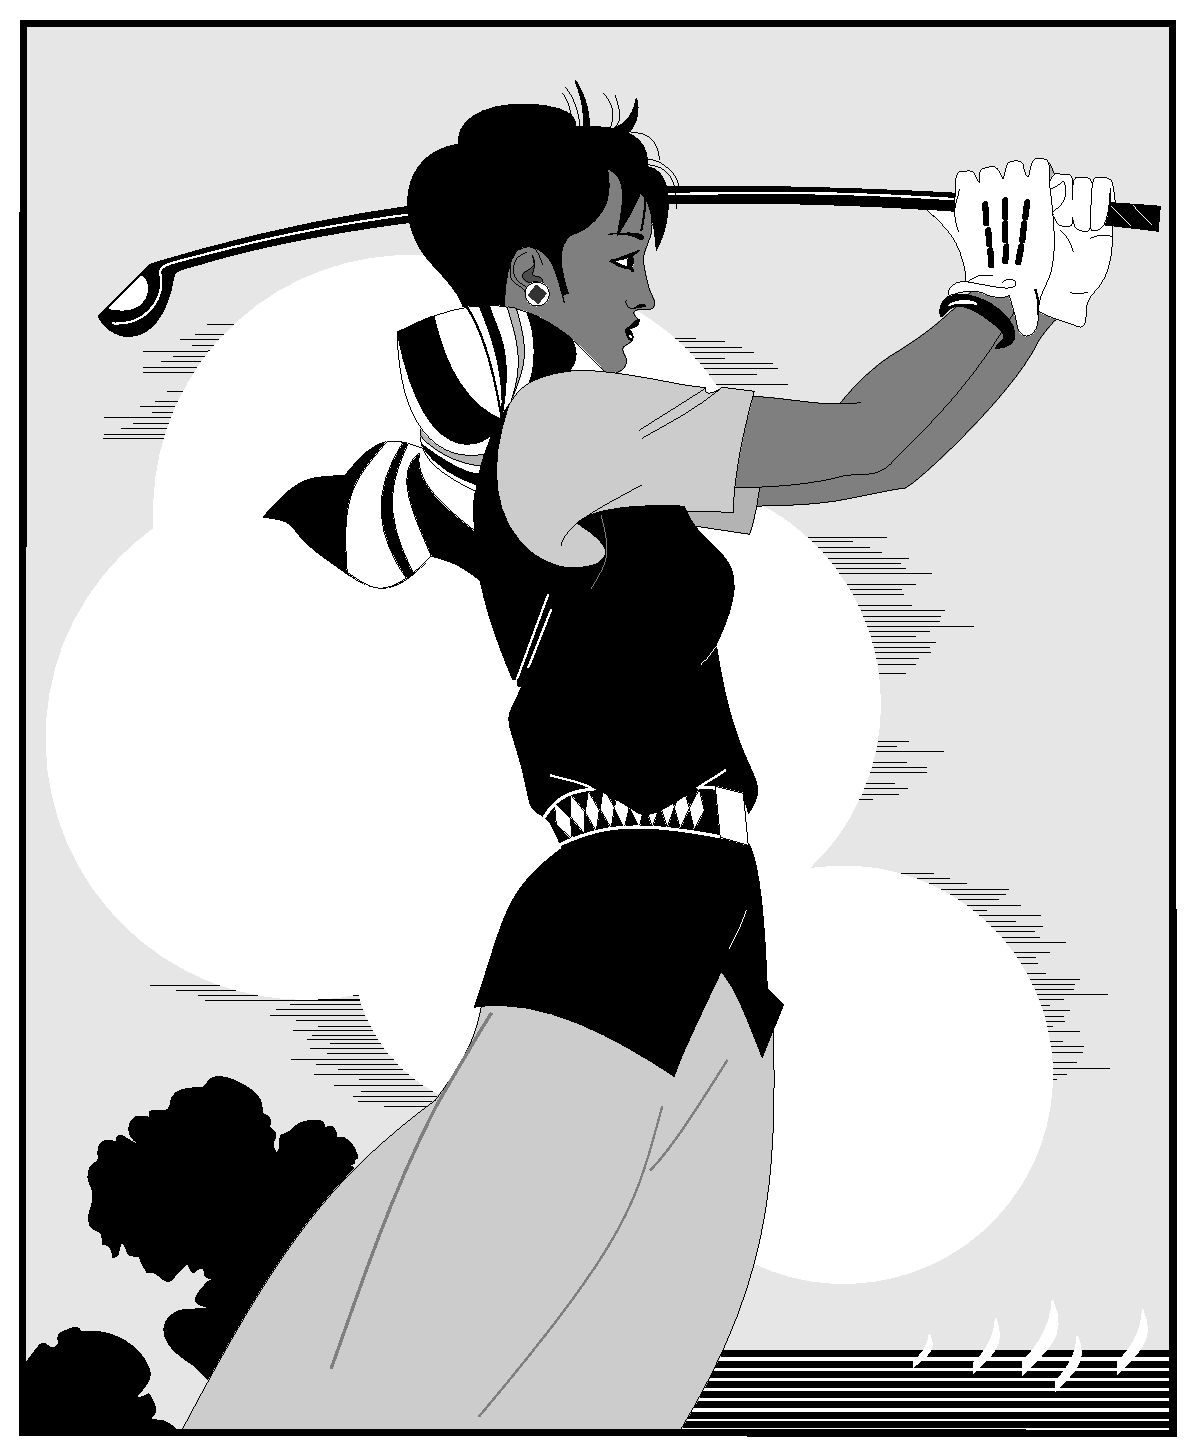
\includegraphics[width = 0.4\textwidth]{golfer}
\FigureBiCaption{打高尔夫球的人}{Golfer}
\label{Figure:Tricks:Example1}
\end{figure}

如果某图题很长的话,可以通过局部改变\verb|\captionwidth|的宽度进行断行。
图~\ref{Figure:Tricks:Example11}给出了一个中英文标题过长的例子。

\begin{figure}[htbp]
\centering
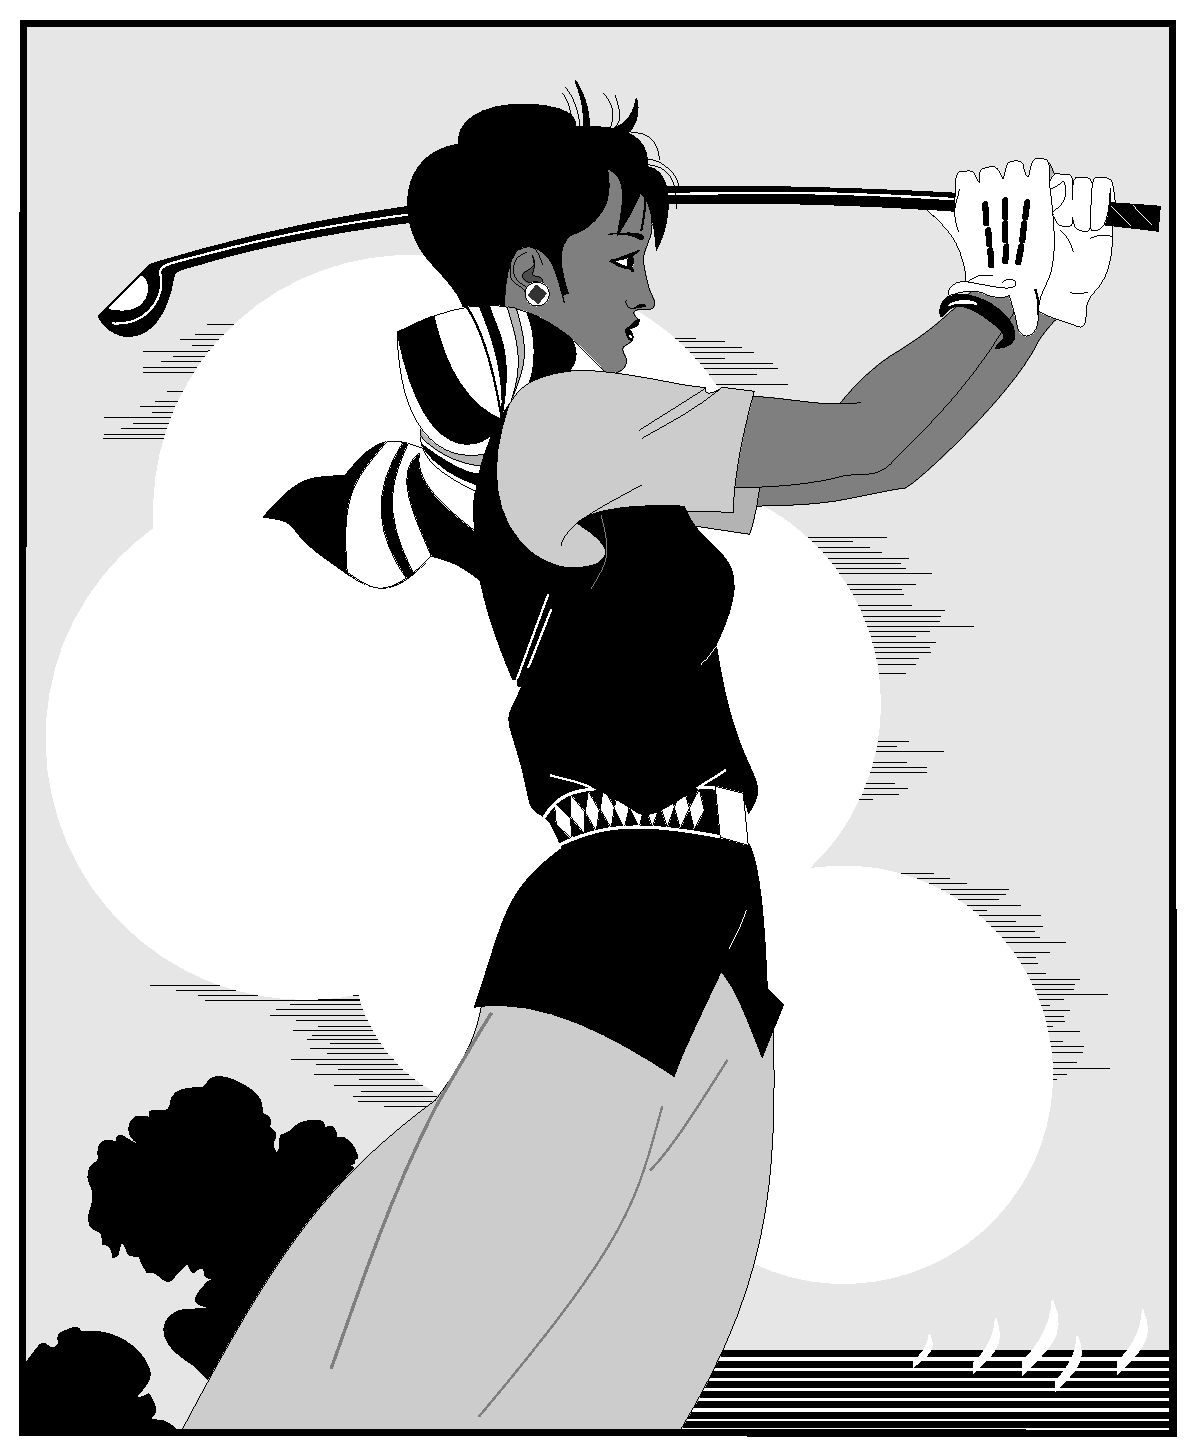
\includegraphics[width = 0.4\textwidth]{golfer}
\changecaptionwidth \captionwidth{0.7\textwidth}
\FigureBiCaption{一个打高尔夫球的人打 高尔夫球的人打高尔打
高尔夫球的人 打高尔 夫球的人打高尔夫球 的人打高尔夫球的
人打高尔夫球的人}{Golfer Golfer This is a very good idea and i
like it very much do u like it Golfer Golfer Golfer Golfer Golfer
Golfer Golfer Golfer Golfer} \label{Figure:Tricks:Example11}
\end{figure}

\normalcaptionwidth
图~\ref{Figure:Tricks:Example12}是恢复默认宽度之后的图形例子。
\begin{figure}[htbp]
\centering
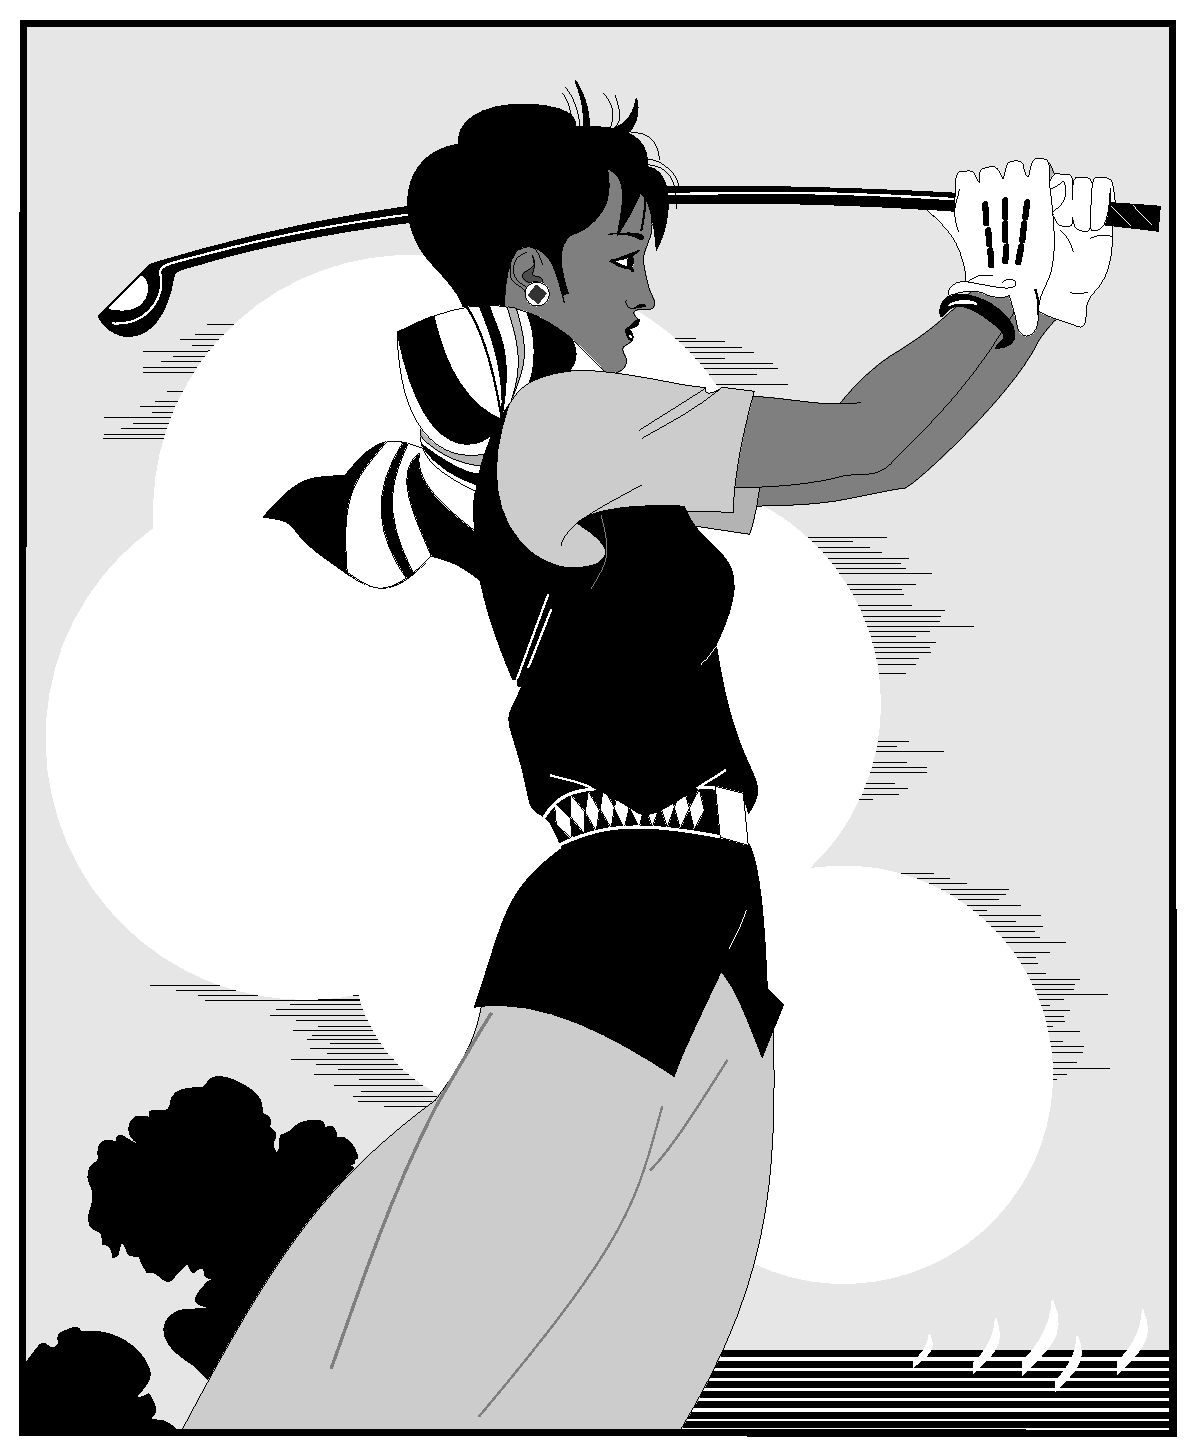
\includegraphics[width = 0.4\textwidth]{golfer}
\FigureBiCaption{打高尔夫球的人打高尔夫球的人打高尔打高尔夫球的人打高尔夫球的人打高尔夫球的人打高尔夫球的人打高尔夫球的人}{Golfer Golfer Golfer Golfer Golfer Golfer   Golfer Golfer Golfer Golfer Golfer Golfer Golfer Golfer Golfer Golfer Golfer Golfer}
\label{Figure:Tricks:Example12}
\end{figure}


为子图定义了一个英文标题命令:
\begin{verb}
\SubfigEnCaption{英文}。
\end{verb}
在紧接着~subfigure~后面用这个命令,参数是英文标题。
当一行不只一个子图时,将图放在~minipage~中,在~minipage~中用这个命令。

图~\ref{Figure:Tricks:Example2} 给出了一行只有一个子图的例子。

图~\ref{Figure:Tricks:Example3} 给出了一行有多个子图的例子。

\begin{figure}[htbp]
\centering
\begin{minipage}{0.40\textwidth}
\centering
\subfigure[高尔夫1]{\label{Figure:Tricks:Example2:a}
  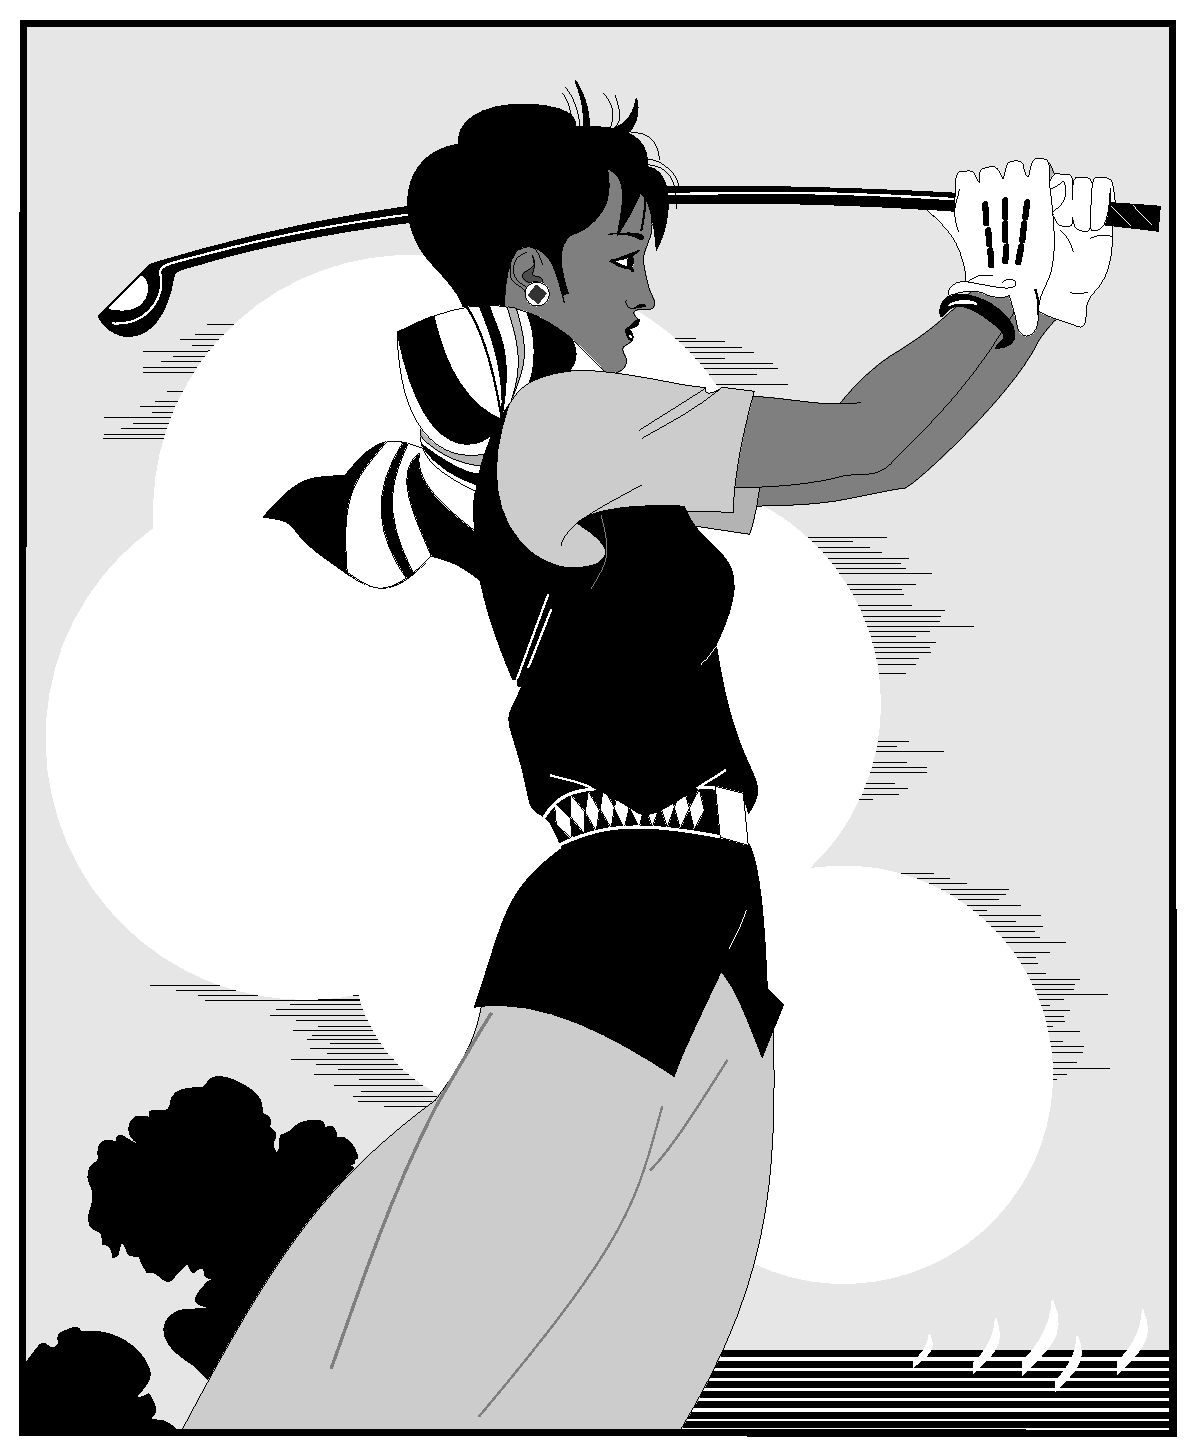
\includegraphics[width = \textwidth]{golfer}
}\SubfigEnCaption{Golfer1}
\end{minipage} 

\begin{minipage}{0.40\textwidth} %
\centering
\subfigure[高尔夫2]{\label{Figure:Tricks:Example2:B}
  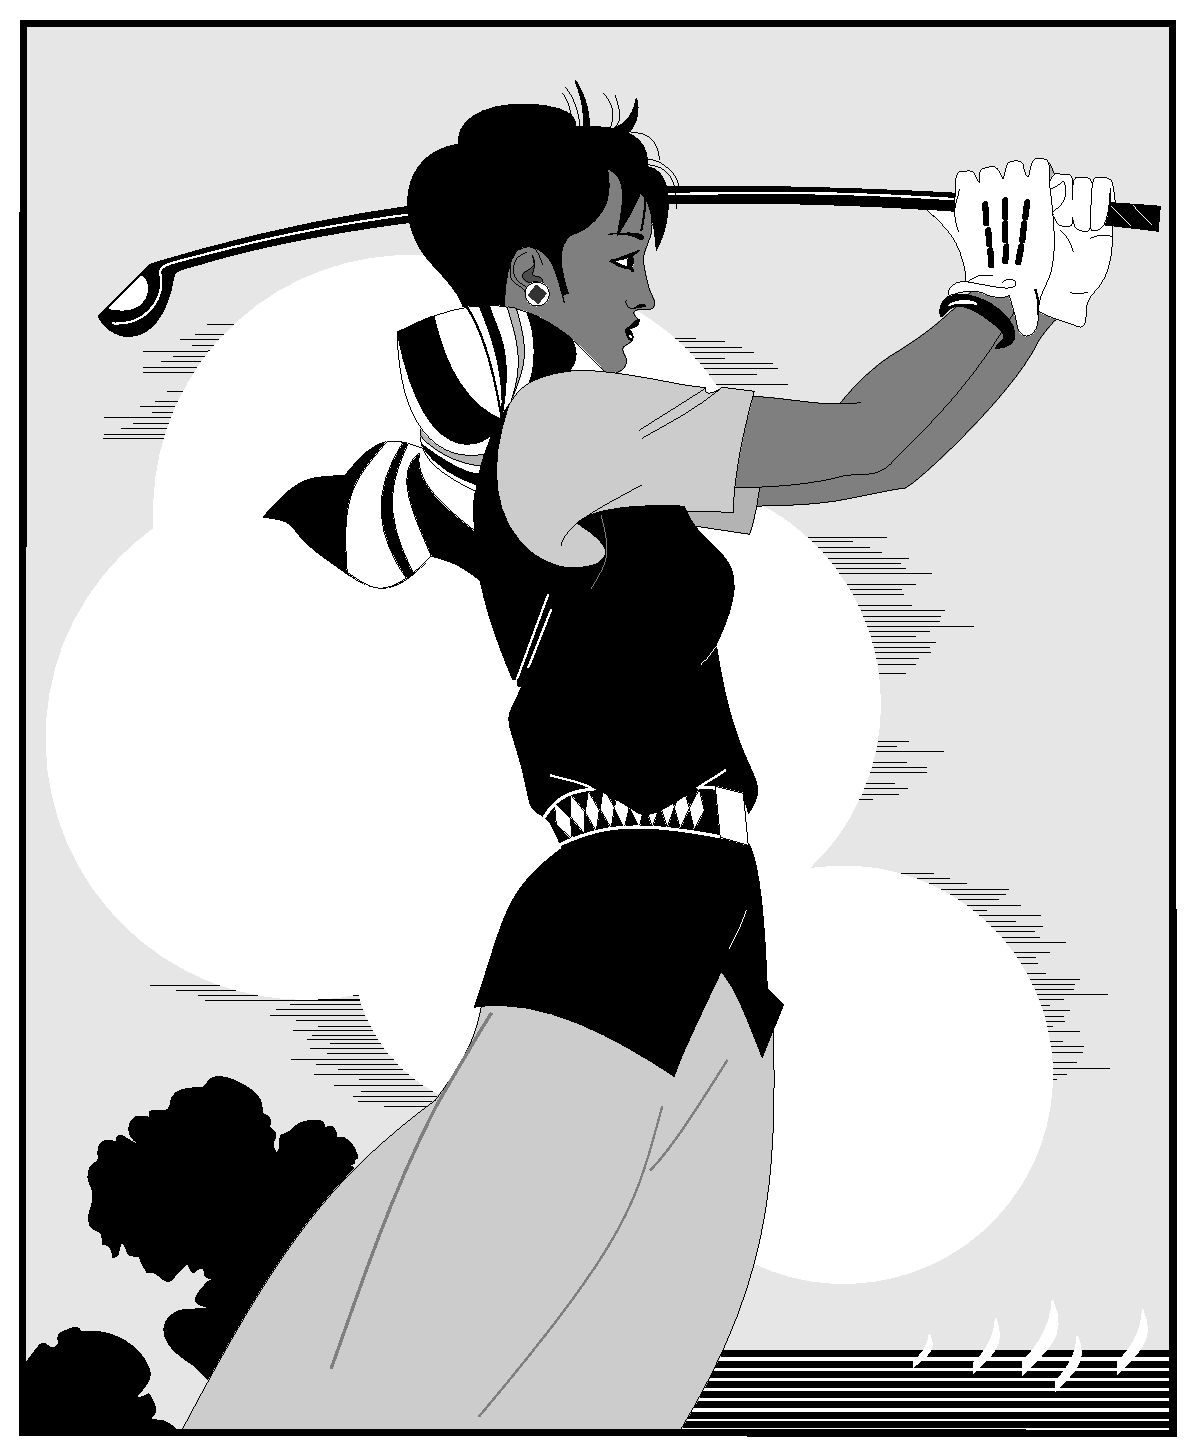
\includegraphics[width = \textwidth]{golfer}
}\SubfigEnCaption{$I_{\rm dc} = 0.5 III$A}
\end{minipage}
\FigureBiCaption{高尔夫}{Golf}
\label{Figure:Tricks:Example2222}
\end{figure}

\begin{figure}[htbp]
\centering
\begin{minipage}{0.25\textwidth}
\centering
\subfigure[高尔夫1]{\label{Figure:Tricks:Example3:a}
  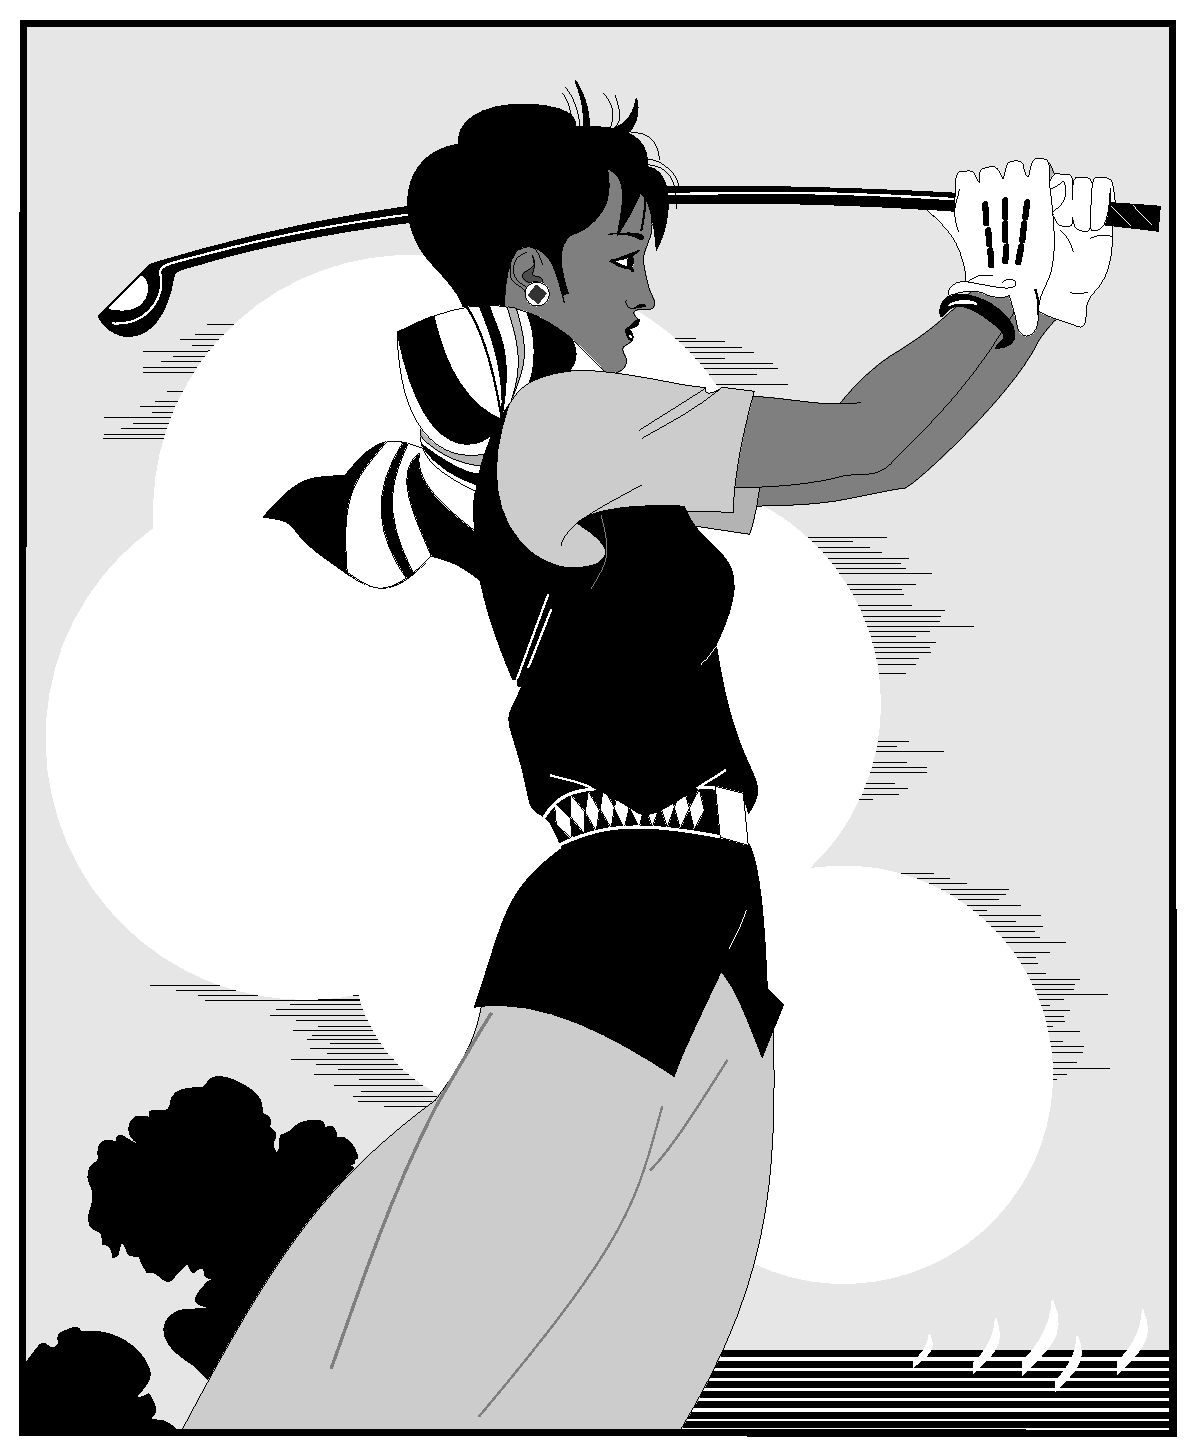
\includegraphics[width = \textwidth]{golfer}
}\vspace*{-5pt}\SubfigEnCaption{Golfer1}
\end{minipage}
\begin{minipage}{0.25\textwidth}
\centering
\subfigure[高尔夫2]{\label{Figure:Tricks:Example3:B}
  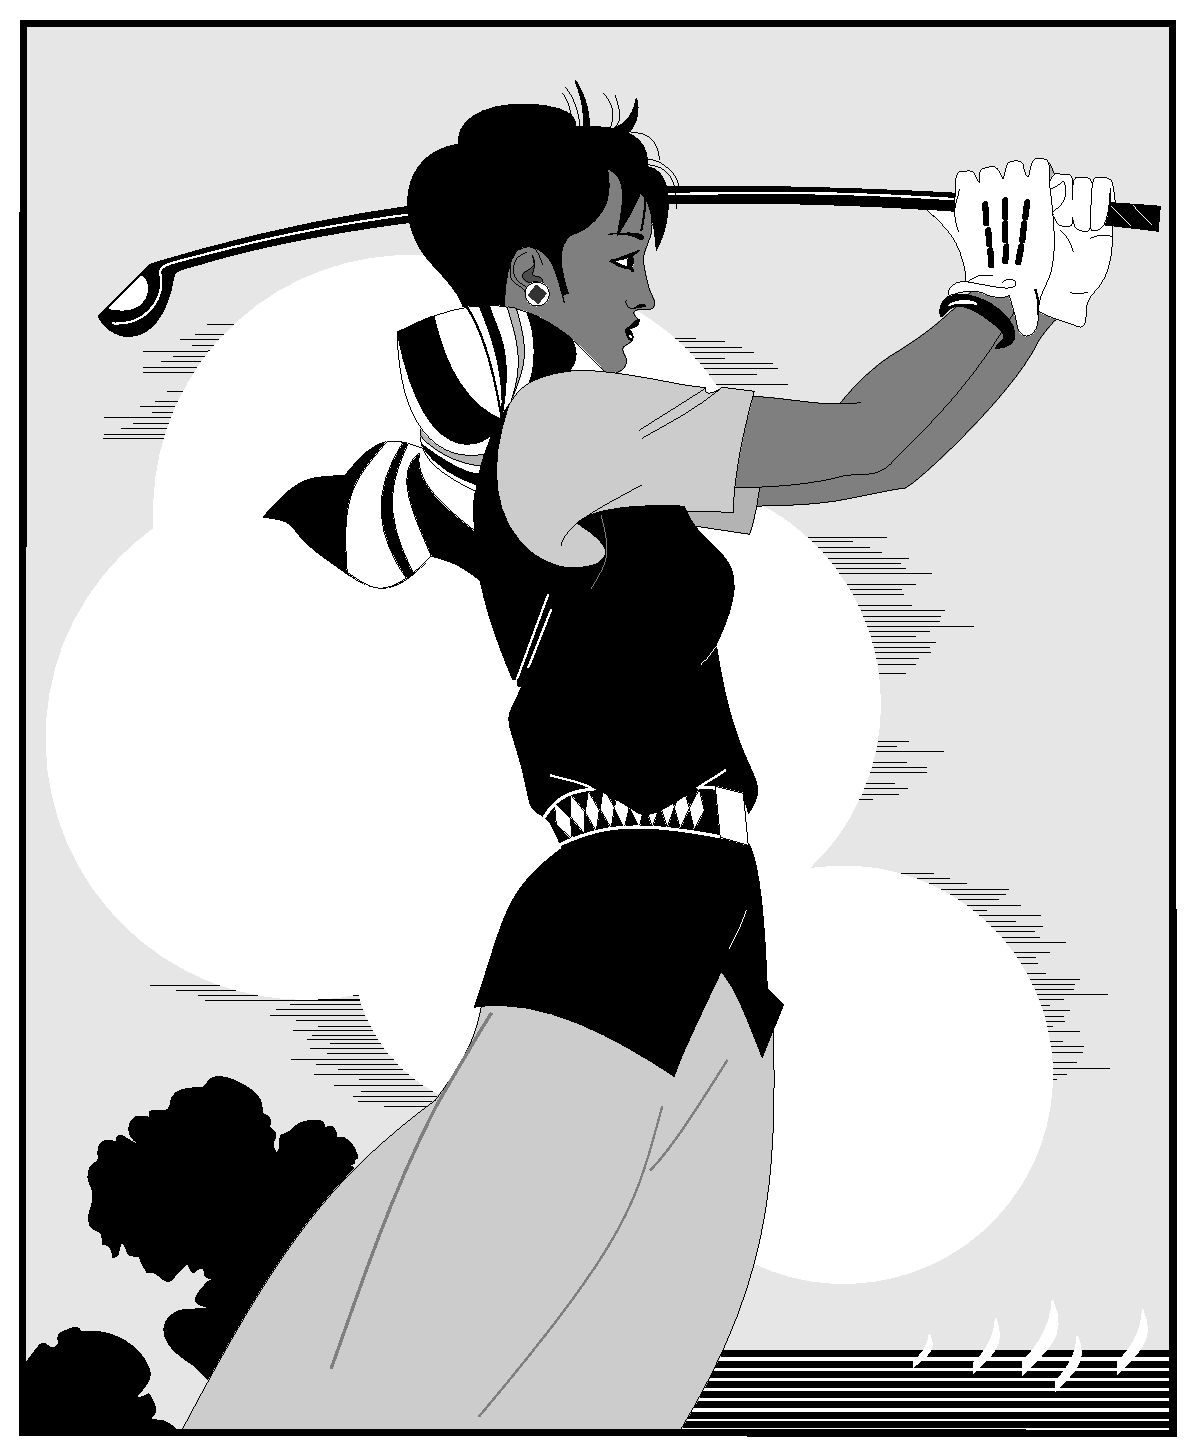
\includegraphics[width = \textwidth]{golfer}
}\vspace*{-5pt}\SubfigEnCaption{Golfer2}
\end{minipage}
\begin{minipage}{0.25\textwidth}
\centering
\subfigure[高尔夫3]{\label{Figure:Tricks:Example3:C}
  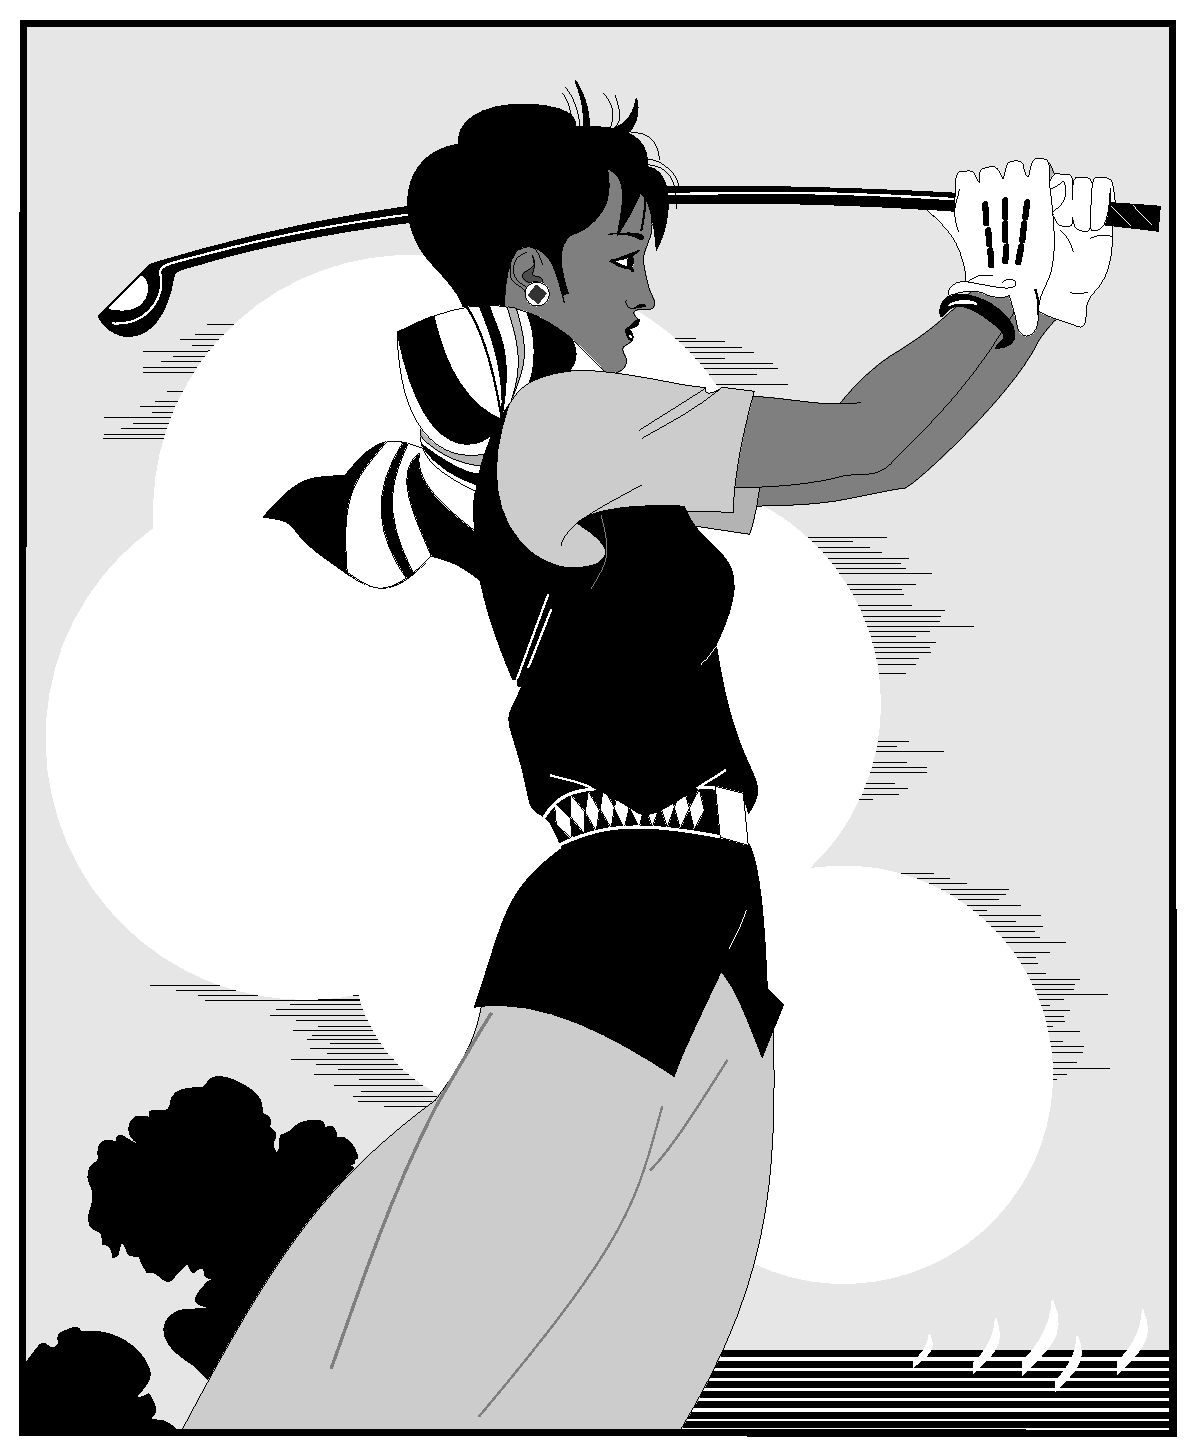
\includegraphics[width = \textwidth]{golfer}
}\vspace*{-5pt}\SubfigEnCaption{Golfer3}
\end{minipage}
\FigureBiCaption{高尔夫}{Golf}
\label{Figure:Tricks:Example3}
\end{figure}

图~\ref{Figure:Tricks:Example3x} 给出了一个不同大小子图的例子,这时可以给出分图的标号,然后把分图的图题
放到母图图题的下面。
\begin{figure}[htbp]
\centering
\begin{minipage}[b]{0.45\textwidth}
\centering
\subfigure[]{\label{Figure:Tricks:Example3x:a}
  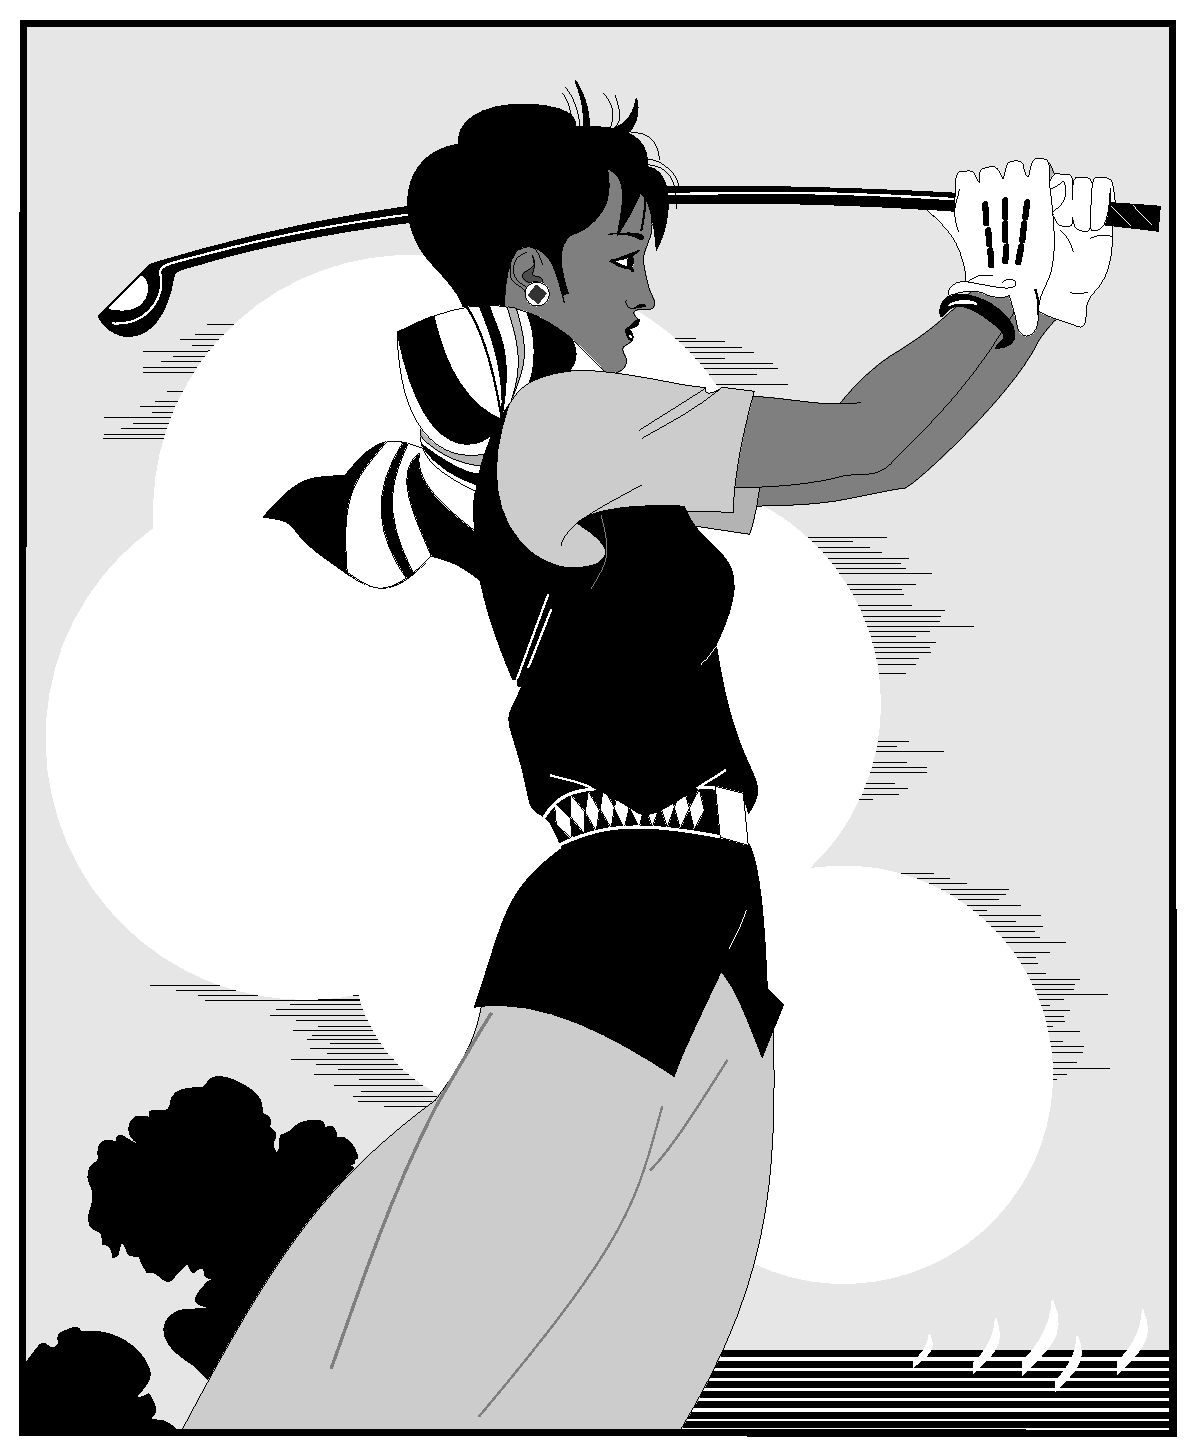
\includegraphics[width = \textwidth]{golfer}
}\vspace*{-5pt}
\end{minipage}
\begin{minipage}[b]{0.15\textwidth}
\centering
\subfigure[]{\label{Figure:Tricks:Example3x:B}
  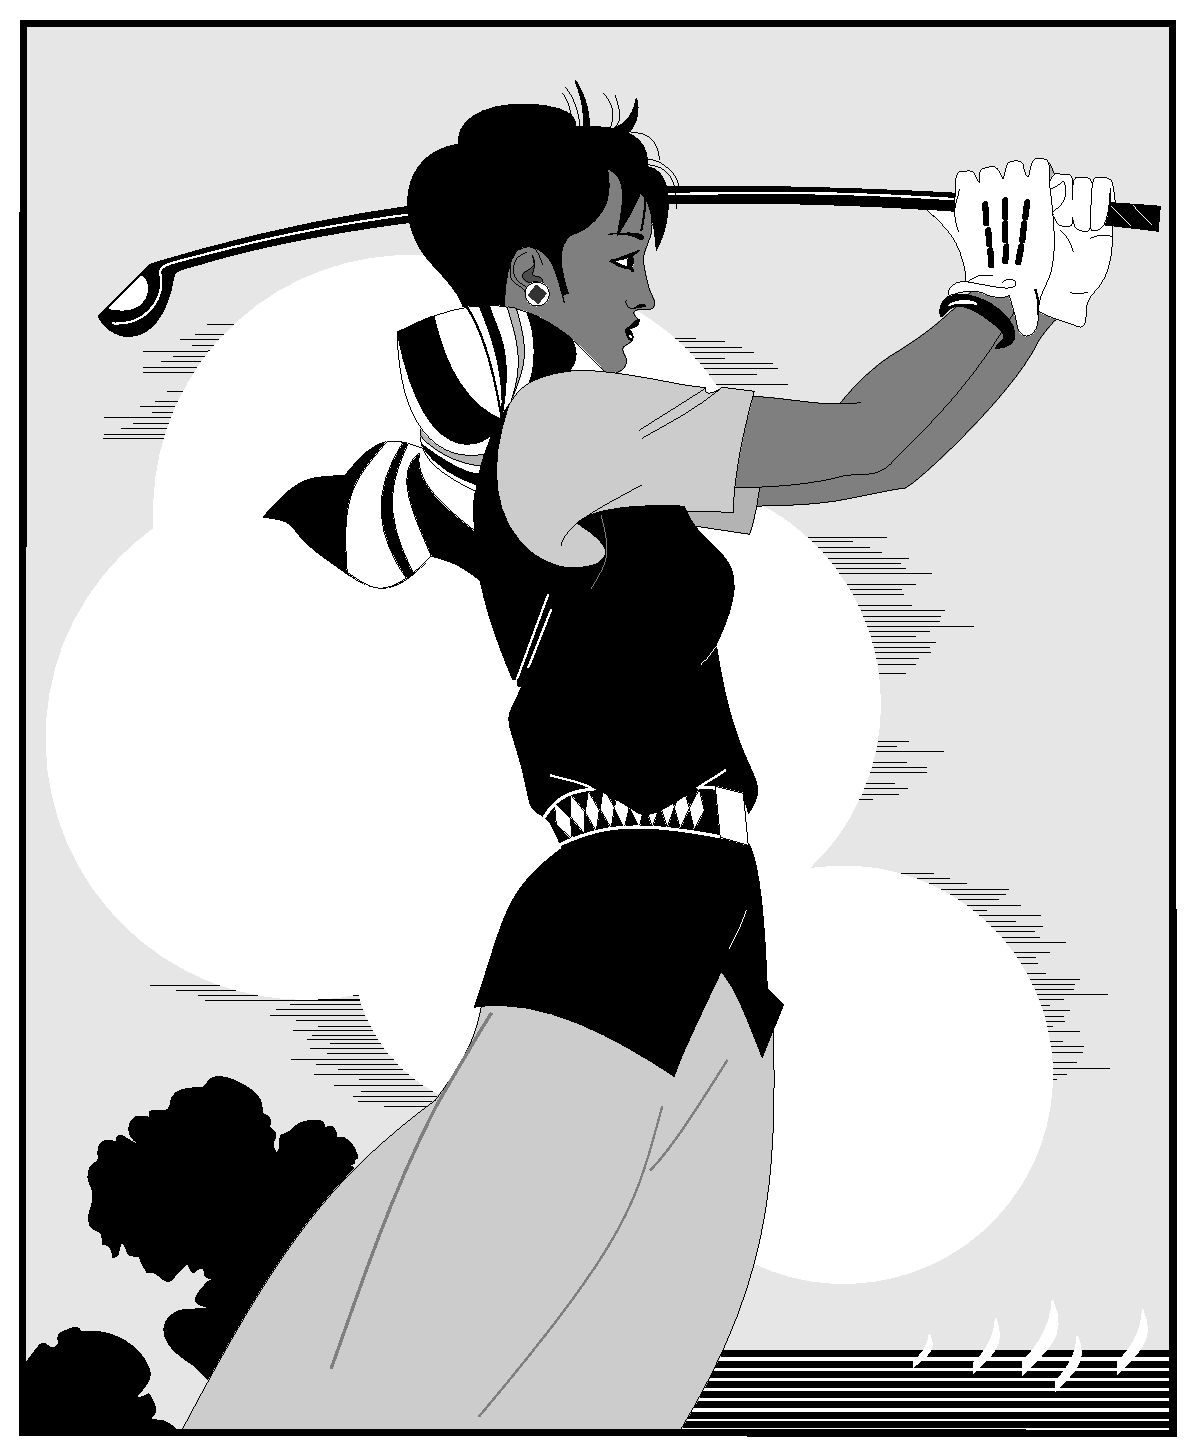
\includegraphics[width = \textwidth]{golfer}
}\vspace*{-5pt}
\end{minipage}
\begin{minipage}[b]{0.15\textwidth}
\centering
\subfigure[]{\label{Figure:Tricks:Example3x:C}
  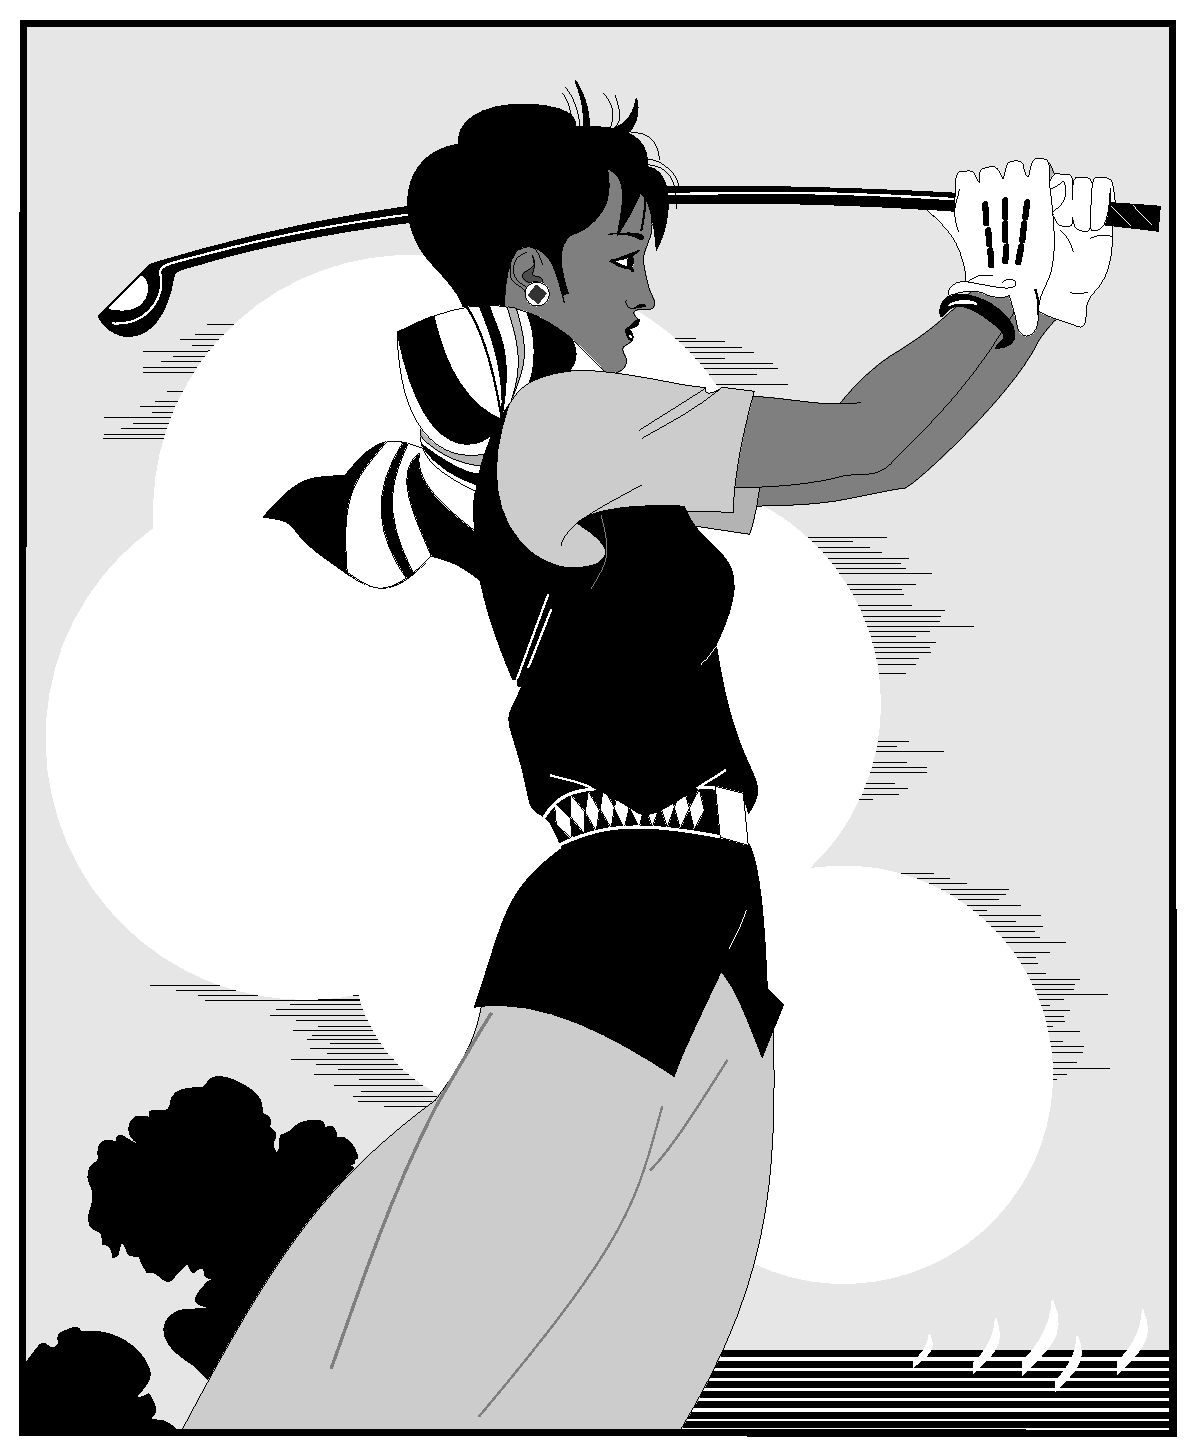
\includegraphics[width = \textwidth]{golfer}
}\vspace*{-5pt}
\end{minipage}
\FigureBiCaption{  高尔夫 \protect \\ a) 分图一; b) 分图二; c) 分图三}%
{  figure caption \protect \\ a) the first subfigure; b) the second subfigure; c) the third subfigure }
\label{Figure:Tricks:Example3x}
\end{figure}


图~\ref{Figure:Tricks:Example31} 给出了一个子图图题过长的例子
\begin{figure}[htbp]
\centering
\begin{minipage}[t]{0.20\textwidth}
\centering
\subfigure[高尔夫高尔夫高尔夫高尔夫1]{\label{Figure:Tricks:Example31:a}
  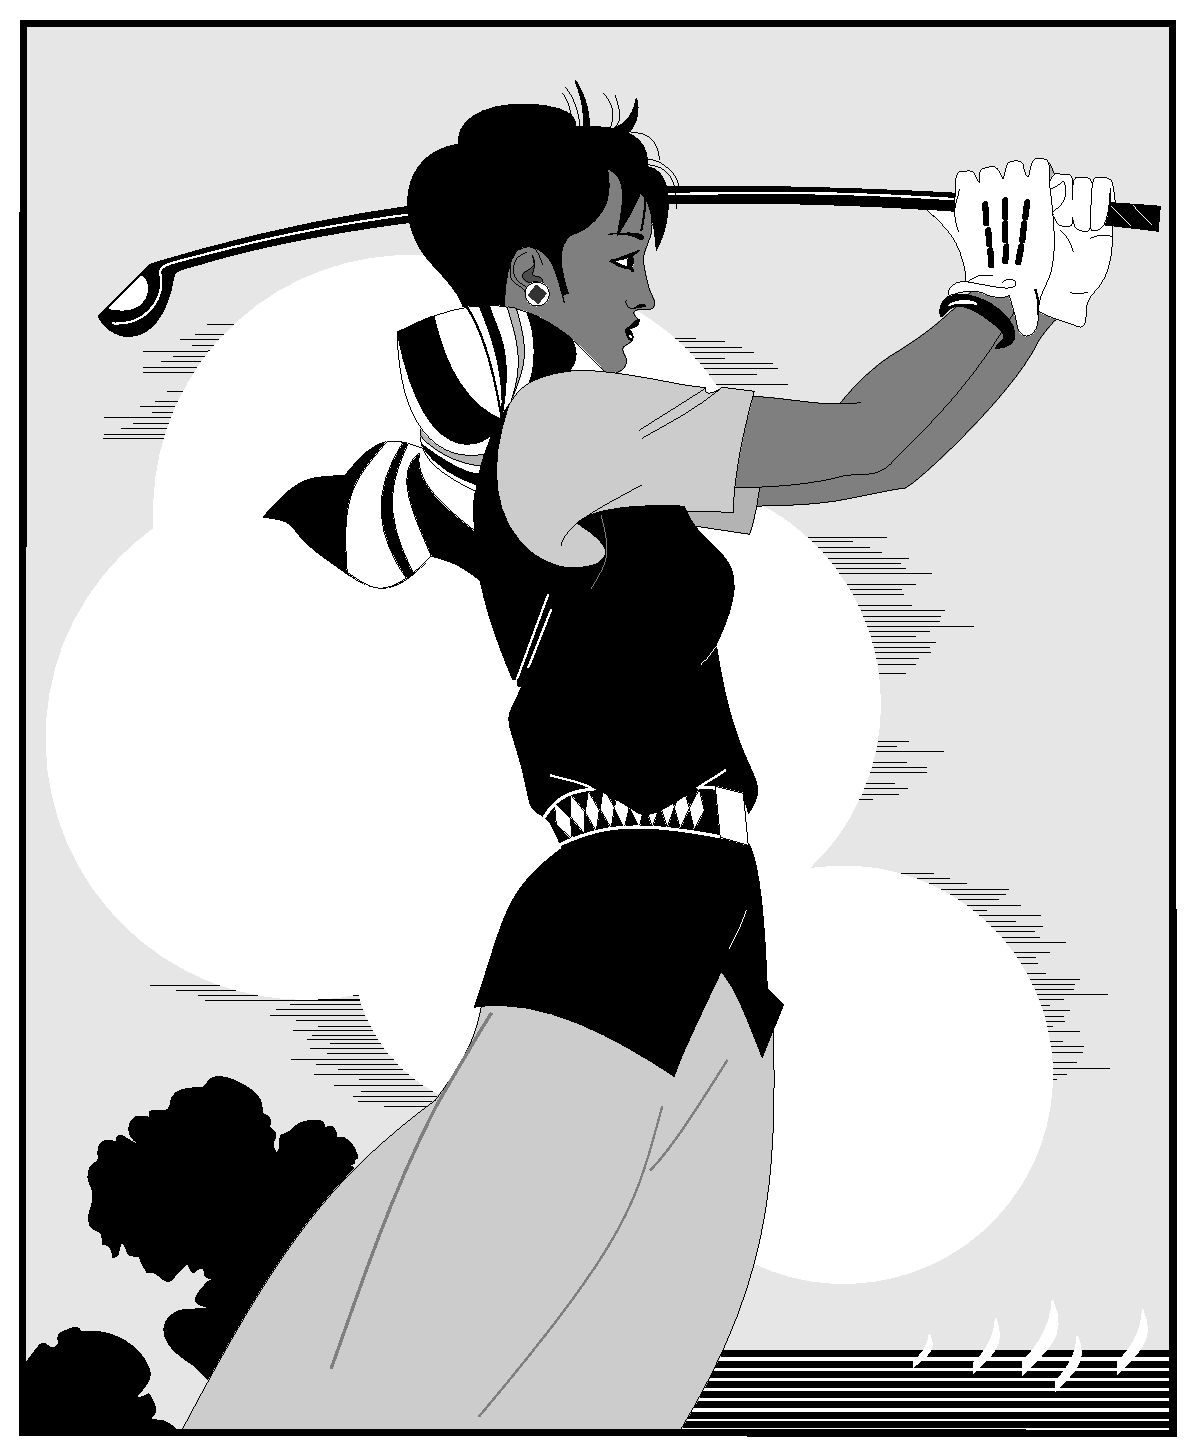
\includegraphics[width = \textwidth]{golfer}
}\SubfigEnCaption{Golfer1 Golfer1 Golfer1 Golfer1 Golfer1}
\end{minipage}\hspace{2em}
\begin{minipage}[t]{0.20\textwidth}
\centering
\subfigure[高尔夫高尔夫高尔夫高夫2]{\label{Figure:Tricks:Example31:B}
  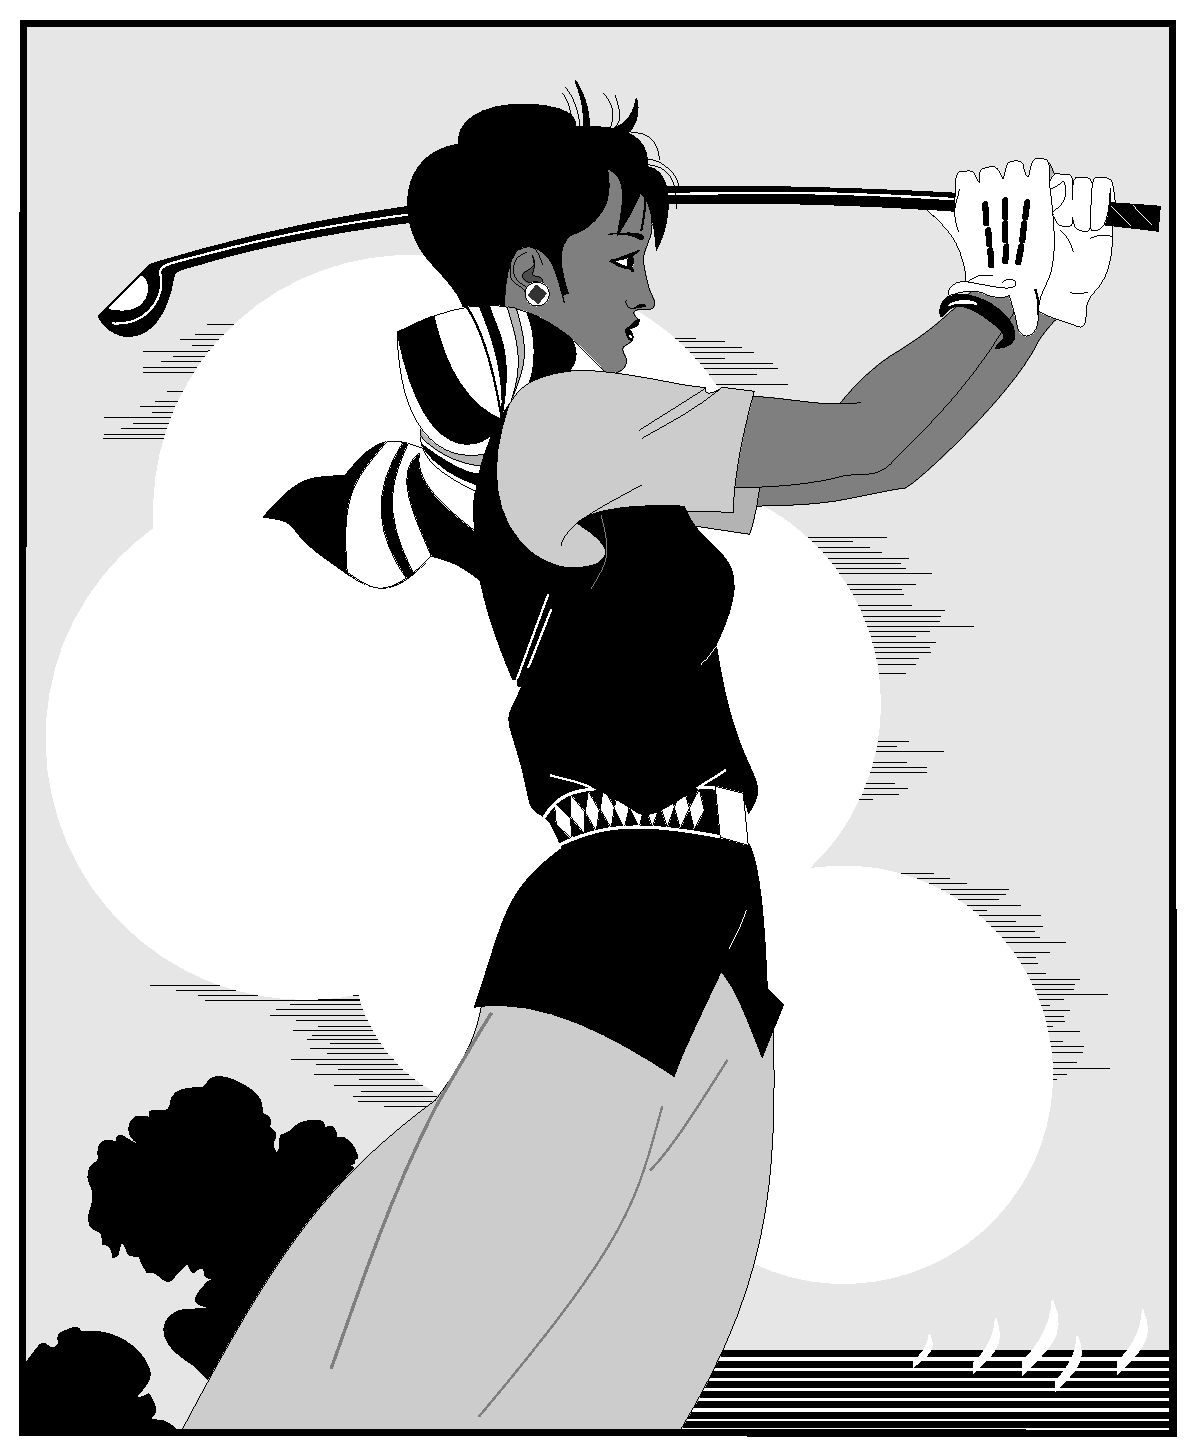
\includegraphics[width = \textwidth]{golfer}
}\SubfigEnCaption{G G f f f f f f f f f f f f f f f f f f}
\end{minipage}\hspace{2em}
\begin{minipage}[t]{0.20\textwidth}
\centering
\subfigure[高尔夫高尔夫高尔夫高尔3]{\label{Figure:Tricks:Example31:C}
  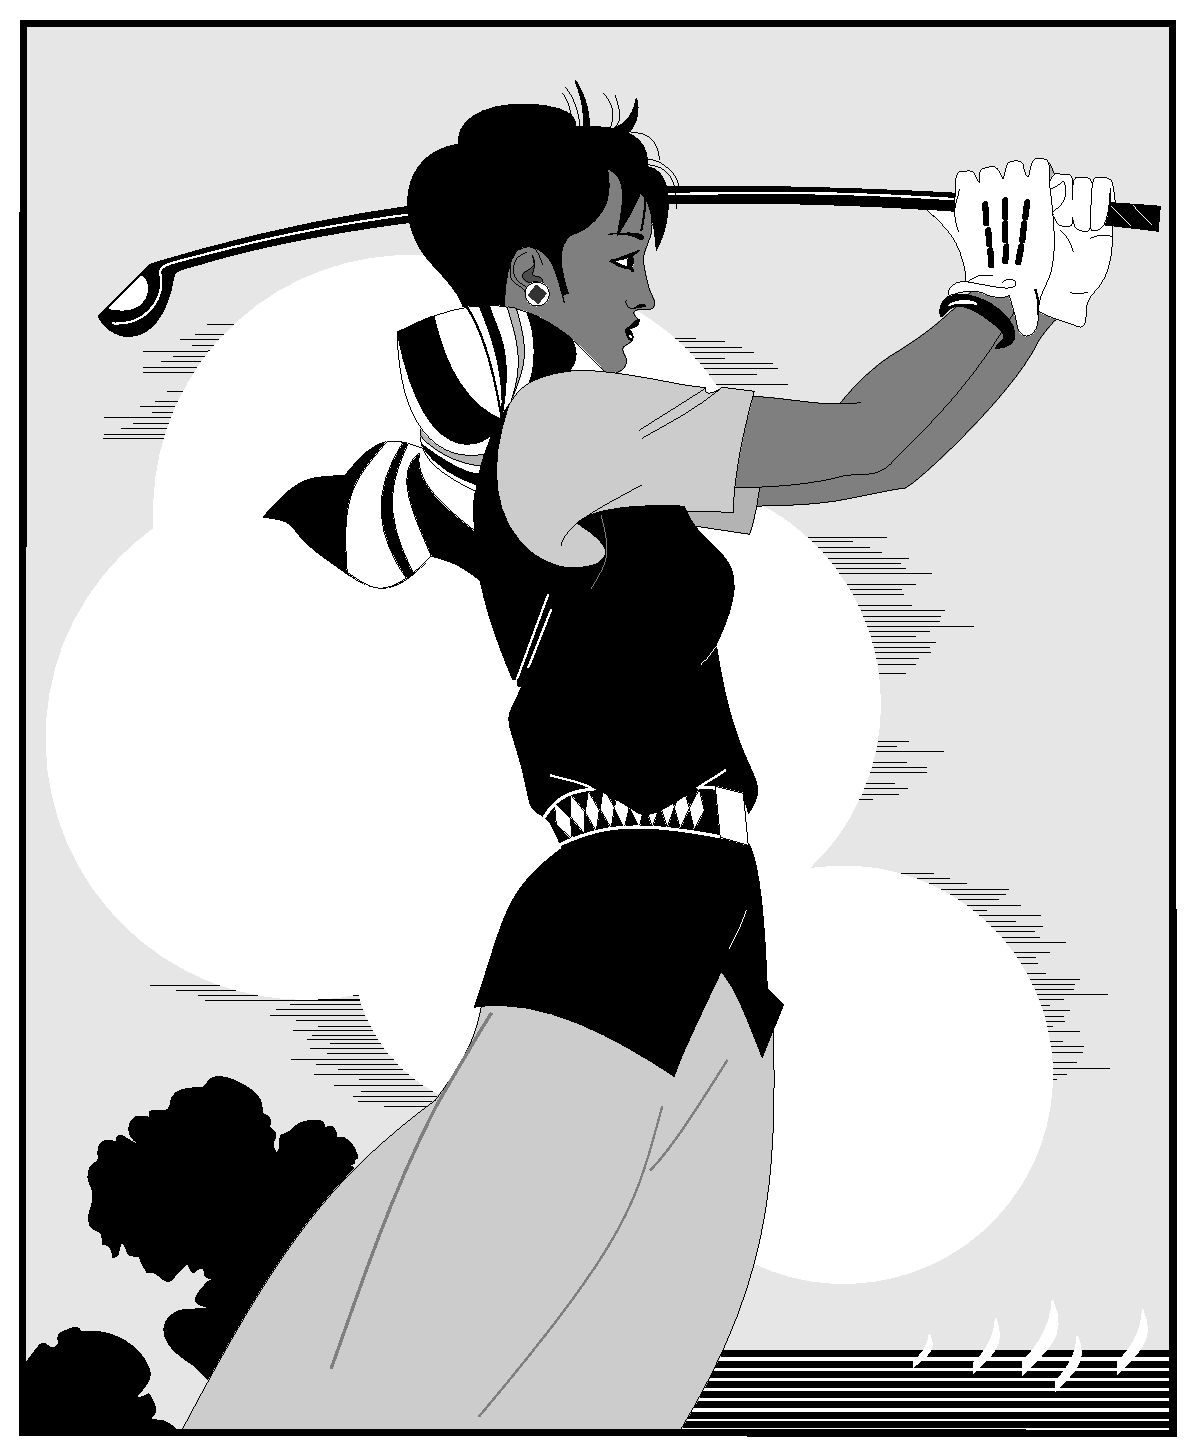
\includegraphics[width = \textwidth]{golfer}
}\SubfigEnCaption{Golfer3 Golfer3 Golfer3 Golfer3 Golfer3 Golfer3}
\end{minipage}
\FigureBiCaption{总图:高尔夫 高尔夫 高尔夫 高尔夫 高尔夫}{Parent: Golf Golf Golf Golf Golf}
\label{Figure:Tricks:Example31}
\end{figure}


\BiSubsection{表标题}{Caption of Tables}
模板中分别为表定义了双标题命令:
\verb"\TableBiCaption{中文}{英文}"。
该命令含有两个参数,第一个为中文标题,第二个为英文标题,效果见~\ref{Tricks:Tab1}。


\begin{table}[htbp]
\centering 
\TableBiCaption{表格测试}{Test of Table}
\label{Tricks:Tab1}
\begin{tabular}{c|c|c}
  \hline
  % after \\: \hline or \cline{col1-col2} \cline{col3-col4} ...
  方法 & 精度~(\%) & 速度~(ms) \\
  \hline
  小波变换 & $99.8$ &  20\\
  傅立叶变换 & $99.0$ & 30 \\
  \hline
\end{tabular}
\end{table}

对于长表格的中英文标题,采用~\verb"\LTBiTocCaption{中文长表短标题(目录中)}{中文长表长标题(正文中)}{Table}{英文长表短标题(目录中)}{英文长表长标题(正文)}"
~来定义。需要注意的是,该命令借鉴了~\verb|ccaption| 宏包中的长表格标题处理方式,含有5个参数,
第三个参数无需改变,由于其他命令限制,参数不容易减少,所以如此定义。
采用这个命令,长表格的标题在正文和图表目录均能正常排版,并且和其他表格的编号协调。
如果需要引用长表格,在~\verb|\LTBiTocCaption|命令之后紧接~\verb|\label| 命令。
表~\ref{table:LTexample} 给出一个例子。

\begin{longtable}{lll} 
\LTBiTocCaption{中文标题短}{中文标题长}{Table}{Long Table  Short Caption}{Long Table Long Caption}\label{table:LTexample}\\
\bfseries Entity & \bfseries Unicode Name & \bfseries Unicode \\ \hline
\endfirsthead
\bfseries Entity & \bfseries Unicode Name & \bfseries Unicode \\ \hline
\endhead
\hline \multicolumn{3}{r}{\emph{Continued on next page}}
\endfoot
\hline
\endlastfoot
a&bcd&bcdef\\
表格&中文文字&中文\\
a&emf&bcdef\\
a&emf&bcdef\\
a&emf&bcdef\\
a&emf&bcdef\\
a&emf&bcdef\\
a&emf&bcdef\\
a&emf&bcdef\\
a&emf&bcdef\\
a&emf&bcdef\\
a&emf&bcdef\\
a&emf&bcdef\\
a&emf&bcdef\\
a&emf&bcdef\\
a&emf&bcdef\\
a&emf&bcdef\\
a&emf&bcdef\\
a&emf&bcdef\\
a&emf&bcdef\\
%a&emf&bcdef\\
\end{longtable}



\BiSection{算法}{algorithm}

这是一个算法的例子,来自~worldguy@lilacbbs。
建议将算法宏包放在minipage环境中,避免算法出现在页面版心之外。

%\begin{algorithm}
%\KwIn{training samples, {$(d_i, d_j)_q$; $\mathbf{q}_i, \mathbf{q}_j \in C$,
%$q\in \mathbf{Q}$} }
%\KwOut{parameter setting $\lambda^T$}%
%
%\For{$t$=1 to $T$}
%{   
%    $\lambda^{t+1}_n = \lambda^t_n + \eta (f_n(q, c, d_i) - f_n(q, c, d_j))$
% }
%\end{algorithm}

算法环境中右侧空白比较多,若想把右侧的空白框减小,可以采用minipage环境实现。把algorithm环境放到minipage环境里面,并且加上选项[H]禁止算法浮动,下面给出一个例子。需要说明的是,一般不需要进行这种处理。算法图题可有可无,若有中英文图题,请使用\verb|\AlgoBiCaption{中文图题}{英文图题}|。下面给出两个有图题的例子。需要说明的是,算法和图表的图题一样,都是自动换行,没有必要手动换行,如果采用\verb|\protect\\|手动换行,会造成目录中也是同样的手动换行,不符合常规排版要求。

\begin{minipage}{0.8\textwidth}\centering
\begin{algorithm}[H]
 \AlgoBiCaption{这是一个简短的算法中文图题}{This is the English caption of the algorithm}
  \KwIn{training samples, {$(d_i, d_j)_q$; $\mathbf{q}_i, \mathbf{q}_j
      \in C$, $q\in \mathbf{Q}$} }
 \KwOut{parameter setting
    $\lambda^T$}
 \For{$t$=1 to $T$} { $\lambda^{t+1}_n = \lambda^t_n +
    \eta (f_n(q, c, d_i) - f_n(q, c, d_j))$ }
\end{algorithm}
\end{minipage}


\begin{minipage}{0.9\textwidth}\centering
\begin{algorithm}[H]
 \AlgoBiCaption{这是一个算法的比较长的中文图题,需要换行,这里采用自动换行,如果手动换行会造成算法目录中同样出现断行}{This is a long English caption of the algorithm, a new line  required, and this a new line}
  \KwIn{training samples, {$(d_i, d_j)_q$; $\mathbf{q}_i, \mathbf{q}_j
      \in C$, $q\in \mathbf{Q}$} }
 \KwOut{parameter setting
    $\lambda^T$}
 \For{$t$=1 to $T$} { $\lambda^{t+1}_n = \lambda^t_n +
    \eta (f_n(q, c, d_i) - f_n(q, c, d_j))$ }
\end{algorithm}
\end{minipage}

\BiSection{公式}{Equations}
\label{Tricks:Equations}

文本中的数学符号和公式用下面的方法输入:

天体力学问题所采取的一个最基本的模型就是通常所说的$N$体问题,即在一
定条件下,所研究的天体被看成质点,$N$体问题最简单的就是二体问题。在一
个天体系统中,$N$个天体往往包含$n$个大天体和$k$个小天体($N=n+k$),其中
$k$个小天体相对$n$个大天体而言小到对后者运动的影响几乎不用考虑,但$k$
个小天体之间可能相距较近,它们之间的相互作用应予考虑,这就构成了限制
性($n+k$)体问题。特别地,当$N=3,~n=2,~k=1$时,即通常所说的限制性三体问题。


最基本的数学公式,带序号的:
\begin{equation}
\ddot{\mathbf{r}}=\mathbf{F}_{0}(r)+\mathbf{F}_{\varepsilon}(\mathbf{r},\dot{\mathbf{r}},t)
\end{equation}
\eqref{eq:noindex}是一个不带序号的例子:
\begin{displaymath}\label{eq:noindex}
F_{\varepsilon}/F_{0}=O (\varepsilon)
\end{displaymath}

\FloatBarrier %清除浮动体
典型的公式加符号说明的例子:

式\eqref{eq:1}为目标飞行器和追踪飞行器之间的相对运动方程
\begin{equation}\label{eq:1}
\ddot{\boldsymbol{\rho}}-\frac{\mu}{R_{t}^{3}}\left( 3\mathbf{R_{t}}\frac{\mathbf{R_{t}\rho}}{R_{t}^{2}}-\boldsymbol{\rho}\right)=\mathbf{a}
\end{equation}
其中:

$\boldsymbol{\rho}$---追踪飞行器与目标飞行器之间的相对位置矢量;

$\ddot{\boldsymbol{\rho}}$---追踪飞行器与目标飞行器之间的相对加速度;

$\mathbf{a}$---推力所产生的加速度;

$\mathbf{R}_{t}$---目标飞行器在惯性坐标系中的位置矢量;

$\omega_{t}$---目标飞行器的轨道角速度;

$\mathbf{g}$---重力加速度,$=\frac{\mu}{R_{t}^{3}}\left(
3\mathbf{R_{t}}\frac{\mathbf{R_{t}\rho}}{R_{t}^{2}}-\boldsymbol{\rho}\right)=\omega_{t}^{2}\frac{R_{t}}{p}\left(
3\mathbf{R_{t}}\frac{\mathbf{R_{t}\rho}}{R_{t}^{2}}-\boldsymbol{\rho}\right)$,这里$p$是目标飞行器的轨道半通径;

公式加符号说明还可以这样:
\begin{equation}\label{eq:111}
\ddot{\boldsymbol{\rho}}-\frac{\mu}{R_{t}^{3}}\left( 3\mathbf{R_{t}}\frac{\mathbf{R_{t}\rho}}{R_{t}^{2}}-\boldsymbol{\rho}\right)=\mathbf{a}
\end{equation}
\begin{formulasymb}{式中}{-15pt}%-3pt,-20pt调与上方的间距。
  \fdesfirst{$\boldsymbol{\rho}$}{追踪飞行器与目标飞行器之间的相对位置矢量;}
  \fdes{$\ddot{\boldsymbol{\rho}}$}{追踪飞行器与目标飞行器之间的相对加速度;}
  \fdes{$\mathbf{a}$}{推力所产生的加速度;}
  \fdes{$\mathbf{R}_{t}$}{目标飞行器在惯性坐标系中的位置矢量;}
  \fdes{$\omega_{t}$}{目标飞行器的轨道角速度;}
  \fdes{$\mathbf{g}$}{重力加速度,$=\frac{\mu}{R_{t}^{3}}\left(
3\mathbf{R_{t}}\frac{\mathbf{R_{t}\rho}}{R_{t}^{2}}-\boldsymbol{\rho}\right)=\omega_{t}^{2}\frac{R_{t}}{p}\left(
3\mathbf{R_{t}}\frac{\mathbf{R_{t}\rho}}{R_{t}^{2}}-\boldsymbol{\rho}\right)$,这里$p$是目标飞行器的轨道半通径;}
\end{formulasymb}

含有矩阵或者向量的公式:
\begin{equation}\label{eq:rho}
\dot{\boldsymbol{\rho}}=\left( \begin{array}{c}
\dot{x}-\omega_{t}y\\\dot{y}+\omega_{t}x\\\dot{z}
\end{array}\right) , \quad
\ddot{\boldsymbol{\rho}}=\left( \begin{array}{c}
\ddot{x}-2\omega_{t}\dot{y}-\omega_{t}^{2}x-\dot{\omega}_{t}y\\
\ddot{y}+2\omega_{t}\dot{x}-\omega_{t}^{2}y+\dot{\omega}_{t}x\\
\ddot{z}
\end{array}\right)
\end{equation}

对于分块矩阵,可以采用~arydshln~宏包,本模板里已经加上这一个宏包支持,使用时遇到问题请参照该宏包自带的文档。
\begin{equation}
A = \left\{ \begin{array}{cc:c} %: 表示竖的虚线;
 x & y & z \\
 u & v & w \\ \hdashline   %横的虚线
 x & y & z
 \end{array} \right\}
 \end{equation}


对于一些较长公式,一行写不下,可以折行:
{\setlength\arraycolsep{2pt}
\begin{eqnarray}
x & = & \left( x_{0}+\frac{2\dot{y}_{0}}{\omega_{t}}+\frac{4a_{x}}{\omega_{t}^{2}}\right) +2\left( \frac{2\dot{x}_{0}}{\omega_{t}}-3y_{0}-\frac{a_{y}}{\omega_{t}^{2}}\right) \sin (\omega_{t} t)- \nonumber\\
& & 2\left( \frac{\dot{y}_{0}}{\omega_{t}}+\frac{2a_{x}}{\omega_{t}^{2}}\right) \cos (\omega_{t} t)-\left( 3\dot{x}_{0}-6\omega_{t} y_{0}-\frac{2a_{y}}{\omega_{t}}\right) t-\frac{3a_{x}}{2}t^{2} \\
y & = & \left( 4y_{0}-\frac{2\dot{x}_{0}}{\omega_{t}}+\frac{a_{y}}{\omega_{t}^{2}} \right) +\left( \frac{\dot{y}_{0}}{\omega_{t}}+\frac{2a_{x}}{\omega_{t}^{2}}\right) \sin (\omega_{t} t) -\nonumber\\
& & \left( 3y_{0}-\frac{2\dot{x}_{0}}{\omega_{t}}+\frac{a_{y}}{\omega_{t}^{2}}\right) \cos (\omega_{t}t)-\frac{2a_{x}}{\omega_{t}}t \\
z & = & \frac{\dot{z}_{0}}{\omega_{t}}\sin (\omega_{t}t)+\left( z_{0}-\frac{a_{x}}{\omega_{t}^{2}}\right)\cos (\omega_{t}t)+\frac{a_{z}}{\omega_{t}^{2}}
\end{eqnarray}}
如果实在没有办法断开,可以用~relsize~宏包中的~mathsmaller mathlarger ,来调整字体,达到缩放的目的,mathsmaller 命令可以反复用多次。

当有连续多个公式时,不要每个公式都用~equation~环境,这样会使得公式之间的距离很大,
推荐使用~align,gather,eqnarray 等环境。
详情请看\href{ftp://ftp.ctex.org/pub/tex/documents/bible/LaTeX_Companion_ch8.zip}{The LaTeX Companion 的第8章}。
前面已经提过,如果你安装的是CTeX套装已经具有此文档。

特殊情况下,需要公式临时左对齐,这时候可以采用模板自定义的~flualign~环境来实现。效果如下:
\begin{flualign}
a=\delta
\end{flualign}

可以通过~\verb"\setlength\jot{距离}"~来设定公式之间的距离,默认为~3pt,该模板将其设定为~8pt。
\begin{gather}
\alpha + \beta = \gamma\\
x^2+y^2=z^2\\
E=mc^2
\end{gather}

\BiSection{一个长的小节标题一个长的小节标题一个长的小节标题一个长的小节标题一个长的小节标题一个长的小节标题}{A Long Section Title Example}\label{tricks:Longsectiontitle}

节\ref{tricks:Longsectiontitle}是一个节标题过长的例子。章标题过长的问题也已经解决,这里给出章标题过长时手动换行的代码。
\begin{verbatim}\BiChapter[这个章标题太长了,需要换行怎么办]{这个章标题太长了,\\需要换行怎么办}
{the chapter title is too long}\end{verbatim}

\BiSection{模板中自定义的一些命令}{Some Commands Defined in the Template}
这里给出模板中自定义的一些命令及简要介绍,详细用法可参照模板中的示例文件~Tricks.tex 等。
\begin{hitlist}
\item \verb+\citeup+~或者~\verb+\ucite+,这是以上标形式引用参考文献;\verb+\cite+常规引用方式
\item 双语章节命令:\verb+\BiChapter, \BiSection, \BiSubsection+\\
\verb+\BiSubsubsection, \BiAppChapter, \BiAppendixChapter+
\item 双语图表命令:\verb+\FigureBiCaption, \SubfigEnCaption+\\
\verb+\TableBiCaption, \LTBiTocCaption+
\item 环境:1、公式描述~formulasymb;2、左对齐公式~flualign;3、列表环境~hitlist、~publist 
\item 中文破折号~\verb+\cdash+;数学模式中输入微分~dx~\verb+\dif+;
\item 表格字号设置命令:\verb+\normalbiao+;\verb+\wuhaobiao+
\item 字号命令:\verb+\yihao, \erhao, \xiaoer, \sanhao, \xiaosan+\\
\verb+\sihao, \xiaosi, \wuhao, \xiaowu+;正文默认字体命令~\verb+defaultfont+
\end{hitlist}


\BiSection{Pluto~模板~FAQs}{FAQs of the PlutoThesis template}
\noindent \textbf{Q1}:\textcolor{blue}{三级标题后重起一段,怎样设置阿?}\\
\textbf{A1}:根据研究生院出的《论文规范》,三级标题后,是接着写而不是像二级标题那样重启一段。如果需要,
可以在~format.tex 中寻找如下代码:
\begin{verbatim}
  \titleformat{\subsubsection}[runin]{\sf\hei\xiaosi}
  {\thesubsubsection}{0.5em}{}[\;\;]
\end{verbatim}
改为:
\begin{verbatim}
  \titleformat{\subsubsection}[hang]{\hei\sf\xiaosi}
  {\thesubsubsection}{0.5em}{}
\end{verbatim}

\noindent \textbf{Q2}:\textcolor{blue}{图题和子图题之间距离怎么调整?感觉有点大}\\
\textbf{A2}:手动吧,\verb+\vspace*{-8pt}\FigureBiCaption+

\noindent \textbf{Q3}:\textcolor{blue}{参考文献中标题的大小写有问题,明明写的大写,怎么转成小写了?}\\
\textbf{A3}:参考文献的标题的实词首字母自动大写,其他字母小写。对于一些特殊词,比如:
\verb+{IEEEtran \LaTeX}+ 应该写成 \verb+{IEEEtran} {\LaTeX}+;$\lambda$ 应该写成
\verb+{$\lambda$}+;BaTiO3~写为\verb+{BaTiO3}+。

\noindent \textbf{Q4}:\textcolor{blue}{子图标题用~[~或~]~符号时,总是出错呀}\\
\textbf{A4}:在用~subfigure~时,如果子图标题含有~[~,需要用~\{~和~\}~包围,比如
\verb+$\beta\in{[0,\,\pi]}$+

\noindent \textbf{Q5}:\textcolor{blue}{请问表格中的顶端和低端的"粗线"怎么打?}\\
\textbf{A5}:原来用两\verb+\hline+的地方,现在用\verb+\toprule+,下面用\verb+\bottomrule+,
或者\verb+\specialrule{1pt}{0pt}{0pt}+。

\noindent \textbf{Q6}:\textcolor{blue}{怎么统计论文的字数?}\\
\textbf{A6}:一般可以用两种方法粗略估计字数。1. dos下运行 charcnt main.dvi,字数~$\approx$~全角字符数~+~其他字符数/5;
2. 将~.pdf 另存为~.rtf 文件,然后用~MS Word~进行字数统计。

\noindent \textbf{Q7}:\textcolor{blue}{各章的图单独放在不同的子文件夹里?}\\
\textbf{A7}:\verb+\graphicspath{{figures/chp1/}{figures/chp2/}}+。

\noindent \textbf{Q8}:\textcolor{blue}{参考文献把~bib~文件中的文献全部列出来了,即使有些文献没有引用的?}\\
\textbf{A8}:在main.tex中查找~\verb+\nocite{*}+~,并去掉。

\noindent \textbf{Q9}:\textcolor{blue}{表格的字号问题?}\\
\textbf{A9}:正文中表格内容默认是五号字,同时模板提供了两个切换命令~\verb+\normalbiao \wuhaobiao+,前者表示命令之后的表格没有字体限定,采用与正文相同的字号;后者强制命令之后的表格采用五号字。

\noindent \textbf{Q10}:\textcolor{blue}{标点出现在行首?}\\
\textbf{A10}:这种情况一般出现在“\verb+英文~标点+”,或者“\verb+数学~标点+”,去掉中间的\verb+~+就行了。书写示例:\verb+control,+、\verb+$a=c$,+。

\noindent \textbf{Q11}:\textcolor{blue}{图表位置的问题?}\\
\textbf{A11}:图表在~\LaTeX~中属于浮动体,~\LaTeX~本身会根据臭度,自行调整浮动体的位置,如果需要把图表在某个位置之前全部排出,可以使用~\verb+\FloatBarrier+命令

\noindent \textbf{Q12}:\textcolor{blue}{Pluto 模板升级的问题?}\\
\textbf{A12}:从~1.8rc2 这个版本开始,模板升级时只需把~setup 目录,gb\_452.cpx, gb\_452.cap,chinesebst.bst Authorization.tex 文件替换掉即可(方便吧:-P);当然最好是先把原来内容做一个备份 :-)

\noindent \textbf{Q13}: \textcolor{blue}{怎么编译模板?编译时需要注意哪些问题?}\\
\textbf{A13}: Windows 下直接运行 make.bat 就可以编
译,linux 下是 Makefile;如果你想采用自己的编译方式,则需要相应修
改 main.tex 中的 \verb+\usewhat+ 参数,各个命令的参数及先后顺序参
照~make.bat 或~makefile;PDF 书签出现乱码,很可能是因为你使用的模板
为GBK编码的,没有运行gbk2uni程序(国内的TeX高手专为中文书签正常显示制
作)。一般编译的顺序为:LaTeX(或pdflatex) $\rightarrow$ bibtex $\rightarrow$
LaTeX(或pdflatex) $\rightarrow$ gbk2uni $\rightarrow$ LaTeX(或pdflatex) ( $\rightarrow$
dvipdfmx(或dvips),这一步由dvi格式得到其它格式,pdflatex不需要),更详
细的步骤请见make.bat或Makefile文件。在texlive和miktex中等非中国网友定制
的系统中一般不含有gbk2uni,因此在模板的\verb|accessories\tools\|下提供
了适合各个系统的gbk2uni程序及其源代码,请将其复制到latex.exe所在
的目录下,然后用命令行使用。

\noindent \textbf{Q14}: \textcolor{blue}{多个附录的问题?}\\
\textbf{A14}: 如果是 1.8.0.20071121(含) 之后的版本,示例如下:
\begin{verbatim}
\defaultfont\appendix
\BiAppChapter{附录一}{the first appendix}
。。。。。
\BiAppChapter{附录二}{the second appendix}
。。。。
\end{verbatim}

\noindent \textbf{Q15}:\textcolor{blue}{文献引用的问题? }\\
\textbf{A15}:\verb+\cite+ 是常规形式引用,\verb+\citeup+或\verb+\ucite+是上标形式引用;

%\fi

%%% Local Variables: 
%%% mode: latex
%%% TeX-master: "../main"
%%% End: 

% -*-coding: utf-8 -*-

\defaultfont

\BiChapter{模板升级、修改记录}{Update Record of the Thesis Model}
\label{Updatelog}

\BiSection{说明}{Introduction}
\label{Update:intro}
为了更加有效的维护该论文模板,特增加此章,用以记录模板所经历的改动,
同时此章也有助于用户更深入的了解该模板。

为了让更多的同学分享到最新的论文模板,建议大家在使用模板时如果对模板
有任何改动或者建议,都别忘了到紫丁香BBS上TeX版把自己发现或建议与大家
分享一下。

本章的记录包括版本升级、bug修复等任何涉及到模板内容的改动。

本模板起初是~Stanley~在~2005~年~\url{http://cvs.hit.edu.cn}~上创立了~Pluto(冥王星)哈尔滨工业大学博士学位论文模板开源项目。200~6年~\url{http://cvs.hit.edu.cn}~迁到了~\url{http://gf.cs.hit.edu.cn},nebula~也随之将该项目转移至此。2008年~2 月  ~\url{http://gf.cs.hit.edu.cn} 出现故障暂停服务,~luckyfox 将项目迁移到~ code.google~网站上,网址为 ~\url{http://code.google.com/p/plutothesis/}。若以后~\url{http://gf.cs.hit.edu.cn}~ 恢复服务,可能两个网站同时更新,不过建议大家在检查新版本时最好两个网站都查看一下。

\BiSection{存在的问题及新版本特色}{Problems to be Solved and the features of the latest version}

当前发布的版本修正了一些网友在使用前期版本时发现的bugs,并且功能更进一步增强,
使用更加方便,建议大家更新到该版本。当前版本目前没有已发现的问题存在。(详细内容请看后面的更新日志。)

其他未知待解决的问题还有赖于大家的使用和发现,共同完善。

\BiSection{版本历史}{The Version history about the template}
本节将对模板的版本号及升级记录及其更新者做一详细的说明。

\begin{hitlist}
\item UFO 模板为~1.0 版本。
\item cucme 模板为~1.1 版本。
\item nebula 模板为~1.2 版本。
\item Stanley 模板为~1.3 版本。
\item nebula 先后完善模板为~1.4、1.5 版本。
\item luckyfox 先后完善模板为~1.6、1.7rc1 版本。
\item jdg 完善版本为~1.7rc2 版本,luckyfox 整理发布。
\item luckyfox and LaTeX 发布~1.7 正式版本。
\item luckyfox and LaTeX 发布~1.8 rc1 版本。
\item luckyfox and LaTeX 发布~1.8 rc2 版本。
\item 做成真正的模板后为3.0版本,之后用``$\pi$''的值作为版本号,以后每升级一次精确度进一位,这是
借鉴\LaTeX{}的版本记录方法,象征着趋于完美。
\end{hitlist}

%%%%%%%%%%%%%%%%%%%%%%%%%%%%%%%%%%%%%%%%%%%%%%%%%%%%%%%%%%%%%%%%%%%%%%%%%%%%%
\BiSubsection{模板的诞生}{The Naissance of the Template}
本模板是网友UFO等(2004)基于清华大学博士论文模板,
按照哈尔滨工业大学论文规范开发的\LaTeX{}论文模板。

%%%%%%%%%%%%%%%%%%%%%%%%%%%%%%%%%%%%%%%%%%%%%%%%%%%%%%%%%%%%%%%%%%%%%%%%%%%%%
\BiSubsection{版本升级至$\gamma$~(by cucme--2005.06.06)}{Version Update $\gamma$~(by cucme--06.06.2005)}
\label{Update:06.06.05}

\BiSubsubsection{章节标号}{Mark of Chapter}
对于没有章标号的章,如结论等,定义了一个相应的命令\verb"\BiAppendixChapter"。

在这些命令中均含有两个参数,第一个为中文题目,第二个为英文题目。与UFO的最大不同在于,本模版直接生成中英文目录。

\BiSubsubsection{列表环境}{List Environment}
本模版将3个传统的列表环境参数作了修改,因此可以直接使用它们。不过有以下问题:
\begin{hitlist}
\item 缩进的具体参数可能有点误差,现在是按两个字$24pt$来缩进的,而实际上应该是两个字加上两个字间距。请朋友们试用后再修改吧。

  还有就是每个列表的item中的非首段没有缩进,我的临时解决办法是使用$2$个全角空格`` ''来模拟缩进。

\item 这是当前hitlist环境的第二个item,上一段就是使用$2$个全角空格`` ''来模拟缩进的。
\end{hitlist}

\BiSubsubsection{参考文献}{Reference}
模板中使用的是紫丁香网友Stanley提供的~chinesebst.bst。作了以下修改:
\begin{hitlist}
\item 修正了引用书籍不输出页码问题
\item 修正了引用博士、硕士论文不输出页码的问题
\item 修正了引用博士硕士论文的学校和学位类别颠倒的问题
\item 引用书籍版次位置不正确的问题
\item 使用缩写期刊名时吞掉"."问题
\end{hitlist}
还存在的问题:
\begin{hitlist}
\item 中文文献作者多于3个时输出的是et al 而不是"等",(我google了一下,貌似要用hooklee编的一个程序fixbbl来搞定,哪位试试吧。)
\end{hitlist}

目前可以这么临时解决修改bbl文件,最后版本的时候把中文出现et.al的地方用``等''代替。
保存一份main.bbl文件,以后用这个文件代替同名文件就可以了。

另外多于三个作者的英文文献没有发现输出不一致的问题,
可以再讨论一下。

%%%%%%%%%%%%%%%%%%%%%%%%%%%%%%%%%%%%%%%%%%%%%%%%%%%%%%%%%%%%%%%%%%%%%%%%%%%%%
\BiSubsection{版本升级至1.2(by nebula--2005.06.28)}{Version Update 1.2 (by nebula--28.06.2005)}
\label{Update:28.06.05}
这次升级主要是把近期关于该模板的一些修改整合进模板,同时增加了一些
介绍性的文字和例子。

\BiSubsubsection{模板内容的修改}{Update on the Content of the Model}
\begin{hitlist}
\item 重写了第一章软件环境介绍部分;
\item 第二章打印部分增加了关于Page Scaling选项的说明;
\item 第二章增加了一些公式的例子;
\item 增加了第三章“模板修改记录”,将校庆版的改动记录进来;
\item 增加了Unix/Linux下的clean方法,增加了一个Makefile文件,\$~make clean即可;
\end{hitlist}

\BiSubsubsection{模板格式的修改}{Update on the Format of the Model}
\begin{hitlist}
\item 在package.tex中把hyperref宏包的设置部分移到最后,避免与其它宏包
的冲突,解决了书签、目录链接不正确的问题;
\item 解决了书签的另一个问题,在点各个使用BiAppendixChapter的附录或
摘要时,标题总是被跳过去的,修改了Definition.tex和format.tex;
\item 解决了“定义”、“性质”等序号错乱的问题,修改了format.tex文件;
\item 去掉了关键字和Key Words后面的冒号;
\item 中文封页下面“研究生”等字按要求改为黑体;
\item 英文封页下边左侧的文字同样改为黑体字;
\item 增添了使用受权书的目录项和书签项;
\item 解决了目录细点、粗点问题,使用的是Stanley提供的方法1和2;
\item 增加了目录abstract后面的空行;
\item 调整目录行距;
\item 解决了CONTENTS和ABSTRACT大写的问题;
\item 调整了目录中点之间的距离使之更符合工大论文要求;
\end{hitlist}

%%%%%%%%%%%%%%%%%%%%%%%%%%%%%%%%%%%%%%%%%%%%%%%%%%%%%%%%%%%%%%%%%%%%%%%%%%%%%
\BiSubsection{版本升级至1.3~(by Stanley)}{Version Update 1.3 (by Stanley)}

在~\url{http://cvs.hit.edu.cn}~上创立了~Pluto(冥王星)项目, 以利于模板的发布和修改。

进行了下面这些修改:
\begin{hitlist}
\item 小小节的标题形式是和段落在一起的,并且不出现在目录中;
\item ``第1章''变成``第~1~章'',原来的在format.tex中已经修改,但是好像
   忘了将后面的删除了,也就是\verb"\chaptername"定义了两次,大家可以看看;
\item main.tex中的格式定义内容都放到了format.tex文件中;
\item 增加了yap使用开关,当为true时,使用yap查看时生成超级链接;
\item 在definition.tex中,增加了中文破折号命令\verb"\cdash",大家可以看看;
\item 页眉``第1章''和``章标题''之间增加了两个空格;
\item 封面的对齐方式等进行了微调;
\item 将format.tex definition.tex package.tex中的一些注释去掉了,
   由于经过多次更改,变得到处都是注释,使得内容比较乱,以后都将更改的
   内容写到ChangLog里面吧;
\item 增加了有章节的附录命令\verb"\BiAppChapter",使用方法参考appA.tex;
\item 增加了hitlist列表环境和publist列表环境;
\item 修改和完善了makefile文件;
\item 修改了各章节的使用说明等;
\item 增加了版权声明章节;
\item 首封增加了工大的logo,谁能贡献一个好点的logo?
\end{hitlist}
%%%%%%%%%%%%%%%%%%%%%%%%%%%%%%%%%%%%%%%%%%%%%%%%%%%%%%%%%%%%%%%%%%%%%%%%%%%%%
\BiSubsection{版本升级至1.4~(by nebula)}{Version Update 1.4 (by nebula)}
解决了linux+TeXlive环境下可能遇到书签乱码的问题,感谢理工大学的Huskier
网友发现该问题并提供了解决方案,感谢水木清华网友snoopyzhao提供的gbk2uni
程序代码。

模板的改动如下:
\begin{hitlist}
\item 增加了一个目录~tools,其中有三个文件,其中有两个是源文件,
gbk2uni是可执行文件,编译环境是gcc 3.2.2,如果运行有问
题请自行编译;
\item 改动了makefile文件;
\item 改动了本文件。
\end{hitlist}
%%%%%%%%%%%%%%%%%%%%%%%%%%%%%%%%%%%%%%%%%%%%%%%%%%%%%%%%%%%%%%%%%%%%%%%%%%%%%
\BiSubsection{版本升级至1.5~(by nebula)}{Version Update 1.5 (by nebula)}
更正了封面页中英文副导师、联合培养导师的格式问题,修正了中文副导师位置注释的
错误,感谢Huskier发现该bug,感谢TeX提出解决方案。

模板改动如下:
\begin{hitlist}
\item 改动了format.tex文件;
\item 改动了cover.tex文件;
\item 改动了本文件;
\item 为了方便shell的自动补齐操作,将makefile的文件名改为Makefile。
\end{hitlist}
%%%%%%%%%%%%%%%%%%%%%%%%%%%%%%%%%%%%%%%%%%%%%%%%%%%%%%%%%%%%%%%%%%%%%%%%%%%%%
\BiSubsection{版本升级至1.6~(by luckyfox)}{Version Update 1.6 (by
luckyfox)}
这里的更新大部分来自~jdg@lilac~的贡献,特别感谢他对本模板的关注。另外,对本次更新做出贡献的还有pineapple,TeX,lofe,luckyfox等。

模板改动如下:
\begin{hitlist}
 \item 增加了一个文件~make.bat~方便用户熟悉在~MSwindows~ 下编译模板的全过程,根据~main.tex~中~\verb|\def\useyap{true}|~还是\verb|\def\useyap{false}|自动选择生成书签的编译命令,减小入门困难,并为全局编译提供方便;
 \item 采用~jdg~修正过的~chinesebst.bst~文件,所有已发现的参考文献问题全部解决;
 \item 增加了~jdg~提出的中英文目录在书签中自动生成的功能;
 \item 增加了~jdg~的中英文图形标题索引的功能;
 \item 解决了TeX@lilac发现章节标题过长引起的目录问题;
 \item 增加了ToTemplateMaintainers.tex一章专门介绍pluto模板维护的一些问题,让用户了解模板维护的一般过程,吸引用户参与模板的维护更新;
 \item 增加了研究生院增加保密管理设置页,这里还有待研究生院论文规范的完善。具体说明见../body/authorization.text头部。
 \item 改动的文件有~main.tex、definition.tex、 package.tex、 format.tex、 Update-Log.tex、
  chinesebst.bst、Tricks.tex~等文件。
\end{hitlist}
%%%%%%%%%%%%%%%%%%%%%%%%%%%%%%%%%%%%%%%%%%%%%%%%%%%%%%%%%%%%%%%%%%%%%%%%%%%%%
\BiSubsection{版本升级至1.7rc1~(by luckyfox)}{Version Update 1.7rc1~(by
luckykfox)}

模板改动如下:
\begin{hitlist}
 \item 修正了长表格标题带来的中英文表格目录混乱的问题;
 \item 中文图表目录``插图'' 和``表格'' 加上空格,与``摘要''等协调;
 \item 调整~make.bat 中的命令,提前把上次生成的~dvi、ps 和~ pdf 文件删除,避免编译失败时误以为是本次的编译的问题;
 \item 修正~libq@lilac 发现的采用~Pineapple@lilac 的授权书与本模板不协调,带来的页眉为“博士期间发表的博士论文”的问题;
 \item 增加cmap宏包,可以制作中文可复制的~pdf 文档;
 \item 采用了标准的~ifpdf 宏包代替~ifpdf 定义;
 \item 增加arydshln宏包,给分块矩阵画虚线;
 \item 修正了libq 发现的授权书的硕博士论文相关的笔误问题;
 \item 把~gb\_452.cpx 和 ~gb\_452.cap 里面的中文图表索引每章后面的空行去掉了,与英文保持一致;
 \item 修正了make.bat中编译时得到的纸型是~letter 而不是~a4 的问题;
 \item 修正了长标题项中没有对齐的问题;
 \item 增加一个~ToDoList文件,方便模板维护者统计bug,决定下一步的工作动向;
 \item 修改宏包~hyperref 的生成书签选项,将~dvipdf 改成~dvips ,hyperref 作者反对使用前者。
 \item 修正~make.bat 中的~dvips 命令,去掉~-Pdf 选项(嵌入字体),这个严重影响生成~pdf 文件的速度,却没有太大必要。
\end{hitlist}
%%%%%%%%%%%%%%%%%%%%%%%%%%%%%%%%%%%%%%%%%%%%%%%%%%%%%%%%%%%%%%%%%%%%%%%%%%%%%
\BiSubsection{版本升级至1.7rc2~(by jdg)}{Version Update 1.7rc2(by jdg)}

模板改动如下:
\begin{hitlist}
    \item figures 目录: hit\_logo.pdf, hit\_logo.eps 替换成矢量的;
  \item chinesebst.bst 改正了两处,修正以前版面上提出的~url 问题;
  \item main.tex 加入~reference.bib for winedt gather 设置,在~winedt 可以使用~tree、gather 等特性;
    \verb|\graphicspath{{figures/}}|(定义所有的~eps 文件在 figures 子目录下)放到~\verb|\begin{document}| 之前,在使用~winedt 块编译的时候有用;第~1 章右开
  \item package.tex 增加 ~\verb|\usepackage{etex}|,增加计数器总数(原来是~256,宏包多,可能不够用),编译需基于~eTeX,因为咱模板计数器使用快超过~256了,如果用户自己在添加几个,编译就出错了。
  \item definition.tex 增加一个环境~formulasymb,用来对公式中的符号进行描述,原模板中与工大论文要求的有出入;重新定义~BiChapter 命令,实现标题手动换行,但不影响目录;调整子图编号,符合工大论文要求;
        增加一个命令~\verb|\dif|,在数学模式中输入微分~$\dif$;调整破折号~\verb|\cdash| 的长度;更新表格目录中长表格超链接失效的问题;
        微调表格标题上下的间距;
  \item format.tex 虽然无法像word一样用难看的黑体英文,但最少也要把 章标题 与小节标题的英文字体一致起来;调整中英文目录,现在1.7rc1中的中文目录,章标题 后产生空白,应该在章标题之前产生;
       增加一个命令~\verb|\citeup| 使显示的引用为上标形式,原来有一个~\verb|\ucite|,但~\verb|\ucite|在~winedt 默认设置里没有提示
            而~\verb|\citeup|就有,当然通过改~winedt,也可以使~\verb|\ucite|有;
  \item 完善~clean.bat, 重写了~make.bat文件,通过识别~main.tex中~\textbackslash usewhat的定义,自动选取合适的编译方式,
       支持~pdfLaTeX、dvips、dvipdfmx 三种编译方式及~yap方式。
  \item 更新本~updatelog.tex 文件;
  \item 新编译的~readme.pdf 替换原来的原来的~readme.pdf 字体嵌入不全,估计有的系统会有问题。
  \item 重新定义 ~\verb"\BiChapter" 命令,允许章标题过长时正文中手动换行,同时目录中自动换行。
\end{hitlist}
%%%%%%%%%%%%%%%%%%%%%%%%%%%%%%%%%%%%%%%%%%%%%%%%%%%%%%%%%%%%%%%%%%%%%%%%%%%%%
\BiSubsection{版本升级至 v1.7~(by luckyfox and LaTeX)}{Version Updatev1.7 (by luckyfox and LaTeX)}

模板改动如下:
\begin{hitlist}
  \item 支持二级图形目录,二级表格目录可以仿照图形目录实现;
  \item 子图形英文标题用法更改,由~\verb|\SubfigureCaption|变成~\verb|\SubfigEnCaption|,并修正此命令解决由此带来的鲁棒性可能不强的问题;
  \item 使用~violetwind@bbs.hit 提供的~linux 下的~makefile;
  \item 章节目录和书签中增加图表目录;
  \item 完善模板使用说明;
  \item 至此,目前已知的~bugs 都已解决,功能也日益完善。
\end{hitlist}
%%%%%%%%%%%%%%%%%%%%%%%%%%%%%%%%%%%%%%%%%%%%%%%%%%%%%%%%%%%%%%%%%%%%%%%%%%
\BiSubsection{版本升级至 v1.8rc1~(by luckyfox and LaTeX)}{Version Update v1.8rc1(by luckyfox and LaTeX)}

模板改动如下:
\begin{hitlist}
  \item 添加硕士学位论文支持,自此后硕博士论文模板合为一体,原硕士学位论文模板放弃维护;
  \item 添加研究生院官方学位论文规范(~doc 和~pdf 版本)到模板的附带文件中;
  \item 增加了针对模板的~WinEdt 的~gather,tree infterace 和自定义章节的关键词高亮正常显示的功能;
  \item 增加了~ xl2latex (从~ excel 表格到~ latex 表格代码的转换文件);
  \item 增加了一些入门的文档介绍及编辑技巧说明;
  \item 增加了对校内的模板现状的说明,提出一些选择模板的建议。
\end{hitlist}
%%%%%%%%%%%%%%%%%%%%%%%%%%%%%%%%%%%%%%%%%%%%%%%%%%%%%%%%%%%%%%%%%%%%%%%%%%

\BiSubsection{版本升级至 v1.8rc2~(by luckyfox and LaTeX)}{Version Update v1.8rc2(by luckyfox and LaTeX)}

模板修正以下bugs:
\begin{hitlist}
  \item 修正bst文件,使参考文献里书籍、学位论文中年份与页码之间是冒号,而不是逗号(参见规范),同时对学位论文进行细化,针对中英两种情况,
中文输出``大学名称论文级别'',而英文输出``论文级别,大学名称'';
  \item 修正图题,表题的字号问题。使用ccaption以来,图题,表题字号一直不正确,主要在format.tex进行修正;
  \item 把原 format.tex 的博硕一些定义,移到 type.tex;同时修正当学科不是engineering的时候,英文封面却始终显示 engineering的 小bug;
  \item 彻底修正附录的页眉问题;( 原因在于fancyhead设置是一个全局的设置,改变局部设置用\verb|\markboth{}{}|,在 Authorization.tex 添加了一项这个。在acknwledgement.tex去除fancyhead
  同时在format.tex页眉部分简化,definition.tex biappchapter去除markboth,没有必要);
  \item 修正硕士单面打印时,图表书签的链接指向问题,并去除单面打印时封面的空白页;
  \item 修正 format.tex 中定理的定义。 定理后面不用冒号;
  \item 修正图形英文标题的缩写, 由 ``Fig'' 改为``Fig.'';
  \item 调整 cmap 宏包的引用位置,适应 miktex 2.5。
\end{hitlist}

模板功能增强主要有:
\begin{hitlist}
  \item 增加CJKpunct宏包,使得中文标点符号的处理,更符合中文习惯;
  \item 取消原先的parlist宏包,采用enumitem(个人认为比parlist宏包强大,好用!),
         同时修正 itemize enumerate description 这些列表项的格式;
  \item 增加导言区使用中文的命令设置;
  \item 调整~main.tex 内容,图标索引分离到~figtab.tex,硕博士一些不同选项分离到~type.tex;
  \item 英文封面的 学科、单位,调整到cover.tex, 无需在format.tex中进行更改, 统一在cover.tex中进行更改,体现LaTeX的样式与内容分离的思想。
   需要注意的是:如果学科,单位中需要换行请用\verb|\newline|,而不是\verb|\\|,两边对齐(充满),用\verb|\hfill|.
  \item 针对WinEdt编辑器,修改swithes.dat,winedt.gdi文件,补充一些关键词,如:\verb|\citeup|,\verb|\ucite|,增强了gather功能;
  \item 增加了对 winedt5.5 中自定义命令在 tree 和 gather 中的 toc 的支持,使用方法见该目录下的文本说明。
\end{hitlist}

文档说明完善主要有:
\begin{hitlist}
  \item 补充论文规范里参考文献示例的条目到模板中,同时完善了正文里参考文献引用的使用说明;
  \item 对 Tricks.tex 中封面内容部分、参考文献部分进行了一些补充;
  \item 对校内TeX资源的连接的介绍做一些修正和补充;
\end{hitlist}

\BiSubsection{版本升级至~v1.8.0.20080228~(by luckyfox and LaTeX )}{Version
Update v1.8.0.20080228 (by luckyfox and LaTeX )}

模板修正以下bugs:
\begin{hitlist}
    \item 在使用dvipdfmx编译时,通过 \AtBeginDvi{\special{pdf:tounicode
        GBK-EUC-UCS2}} 可以不用gbk2uni.
        但使用hyperref宏包时,其unicode选项会使 GBK-EUC-UCS2失效,为此去掉
        unicode选项。 其他编译方式 仍需gbk2uni。
    \item 解决 muzak@lilacbbs 提出的 中英摘要关键词过长,
换行时不能自动缩进的问题。 为此在format.tex 对关键词加上悬挂缩进。
    \item 修正论文中url的网址与正文字体不同的bug,并给出一例;
    \item 修正多个附录时,英文目录存在的问题,都是Appendix A;
    \item 更正参考文献 书的版次问题 , reference.bib 中文书edition={第二版},英文书 edition={2nd}
    \item violetwind@hit  改进英文子图图题居中
    \item 修正 chinesebst.bst 文件 对英文硕士论文的处理,输出顺序与博士论文一致,先是学位级别,后是学校。
    \item 精调一下 中英图题间的行距 -1.3ex ;
    \item 重新设定公式与上下文的间距,原先是12pt,现改为10pt
    \item 解决由muzak提出的 当使用子图标题中包含公式符号时编译出错的问题。
原因:加入目录时 \verb|\xdef| 与\verb|\protect| 命令不兼容。 使用LaTeX中的 \verb|\protected@xdef|  代替原来的\verb|\xdef|。
具体参见TeX FAQS: \url{http://www.tex.ac.uk/cgi-bin/texfaq2html?label=edef}
	\item 硕士论文封面问题
	\item 章标题中的数学符号在正文和目录中加粗;节标题中的数学符号在正文中加粗,在目录中不加粗
	\item 中英目录中章标题后粗点还是细点?模板中提供了两种方案,现在采用细点方案,即中英目录中章标题后全部采用细点,中英一致!
	\item 增加两个表格字号切换命令,\verb+\normalbiao+~正常字号;\verb+\wuhaobiao+~五号字。 正文中默认使用\verb+\wuhaobiao+ 。
表格前后无需 \verb+\wuhao,\defaultfont+, 老用户替换 format.tex 即可。
  \item 修正了算法的标题编号问题,和样式问题。
\end{hitlist}


模板功能增强主要有:
\begin{hitlist}
  \item 将原 EditTools tools ThesisCriterion 归到 Accessories 目录里,规范附属文件;
  \item 删除原先algo.sty宏包,采用新算法宏包 algorithm2e,例子直接用的版面上worldguy提供的;
  \item colorlinks 由true全改成 false 吧, 毕竟用 false的人多一些;
  \item 参考文献标题自动大小写功能补充: 添加了三个虚词 via vs its,去掉不常用的 can;
  \item 增加 booktabs 宏包,用于做三线表格;
  \item 精简definition.tex 去除多余的 \verb|\makeatletter,\makeatother| ;
  \item 调整模板的版本标号形式,为*.*.*.*的形式,如1.8.0.20070910。编号规则是:其中第1位是大编号,如果研究生院对论文规范做大规模的调整,论文模板跟进,那么加1;第2位是小编号,如果有很多bugs修正,或者是功能结构上大的调整,则加1,第3位是一些小bug修正后,很快就发布的版本;后面的是模板发布的日期,方便网友使用,也方便管理员查看;
  \item 增加~relsize~宏包,方便调整个别公式字体大小;增加一个环境~flualign~,用于公式左对齐。
\end{hitlist}

文档说明完善主要有:
\begin{hitlist}
  \item 完善文档,增加 一小节,模板 FAQs;
  \item 参考文献 针对中英书籍版次,增加两个例子;
  \item 本次 bug 修正时,有些格式的调整在文档说明的正文中同时做了说明。
\end{hitlist}

%%%%%%%%%%%%%%%%%%%%%%%%%%%%%%%%%%%%%%%%%%%%%%%%%%%%%%%%%%%%%%%%%%%%%%%%%%
\BiSubsection{版本升级至~v1.8.1.20080528~(by luckyfox and LaTeX )}{Version
Update v1.8.1.20080528 (by luckyfox and LaTeX )}

模板修正以下bugs:
\begin{hitlist}
    \item 允许公式出现在页面顶部;
    \item 增大表格内行距;
\end{hitlist}


模板功能增强主要有:
\begin{hitlist}
    \item 增加主要符号表;
\end{hitlist}

文档说明完善主要有:
\begin{hitlist}
   \item 在说明文档中加上google的版本库地址;
   \item 增加红色的版本更新的提醒。
\end{hitlist}

%%%%%%%%%%%%%%%%%%%%%%%%%%%%%%%%%%%%%%%%%%%%%%%%%%%%%%%%%%%%%%%%%%%%%%%%%%
\BiSubsection{版本升级至~v1.8.2.20080601~(by luckyfox and LaTeX )}{Version
Update v1.8.2.20080601 (by luckyfox and LaTeX )}

此版本特别为庆祝六一儿童节,愿我们都保持一颗童心,开心快乐,真诚永远!

模板修正以下bugs:
\begin{hitlist}
    \item 目录页码加上小横线,和正文格式一致;
\end{hitlist}


模板功能增强主要有:
\begin{hitlist}
    \item 保持文件 GBK 编码的同时,增加对 xetex 的支持。
\end{hitlist}

文档说明完善主要有:
\begin{hitlist}
   \item 补充对 xetex 的一些简单说明;
   \item 修改推荐的软件信息,删除对 chinatex 的推荐,增加 MiCTeX 和 MiKTeX 软件。
\end{hitlist}
%%%%%%%%%%%%%%%%%%%%%%%%%%%%%%%%%%%%%%%%%%%%%%%%%%%%%%%%%%%%%%%%%%%%%%%%%%%
\BiSubsection{版本升级至~v1.8.3.20081210~(by luckyfox and LaTeX )}{Version
Update v1.8.3.20081210 (by luckyfox and LaTeX )}

模板修正以下bugs:
\begin{hitlist}
    \item 文件头部加入编码信息;
    \item 跨页表格,标题宽度,末行居中;
    \item 消除Introduction.tex中 \textbackslash section的\} 前没有空格导致出现的hyperref宏包相关错误; 
    \item jdg发现并修正五号表表格未能真正居中对齐的bugs;
    \item 修正UTF编码下某些注释的文字不完整;
    \item 修正子图标题中的字号非5号字的问题; 
    \item 修正utf8的main.tex中原由gbk转换时部分文字无法显示的小bug;
    \item [GBK+UTF8]将jdg针对多个子图并列时子图中英文caption可能不对齐的bug修正的子图英文caption定义代码加入;
    \item 增加gb\_452\_UTF8文件;
\end{hitlist}


模板功能增强主要有:
\begin{hitlist}
    \item 默认编译改成dvipspdf;
    \item 上传xelatex版本的readme,字体比较均匀;
    \item 创建PlutoThesis的utf8文件;
    \item 上传参考文献国标2005文件;
\end{hitlist}

文档说明完善主要有:
\begin{hitlist}
   \item  updatelog的更新
\end{hitlist}
%%%%%%%%%%%%%%%%%%%%%%%%%%%%%%%%%%%%%%%%%%%%%%%%%%%%%%%%%%%%%%%%%%%%%%%%%%
\BiSubsection{版本升级至~v1.9.0.20081213~(by luckyfox and LaTeX )}{Version
Update v1.9.0.20081213 (by luckyfox and LaTeX )}

模板修正以下bugs:
\begin{hitlist}
    \item 修正makefile,添加xelatex编译代码; 
    \item 去掉GBK封面上的"专业",英文封面的 in \textbackslash exueke; 
    \item 修改了版芯,部分尺寸调整还待验证; 
    \item 将英文目录的章改为四号字; 
    \item 第四级标题题序顶格写,与标题空一格,阐述内容另起一段; 
    \item 修正xelatex编译时,英文粗体采用了粗体,而非Times New Roman的bug;
    \item UTF8,修正xelatex编译中文乱码的bug,去掉hyperref的unicode选项; 
\end{hitlist}


模板功能增强主要有:
\begin{hitlist}
    \item 提交比较符合GBT7714-2005标准的bst文件,文件名加后缀"\_HIT"; 
    \item 中文封面加上学校代码和密级; 
    \item 加入新论文规范的readme.pdf;
    \item 添加jdg制作的chinesebst2005,包括GBK和UTF8编码;
    \item 根据参考文献标准要求,修改了Reference.bib文件完善示例文献条目;
\end{hitlist}

文档说明完善主要有:
\begin{hitlist}
   \item  updatelog的更新
\end{hitlist}
%%%%%%%%%%%%%%%%%%%%%%%%%%%%%%%%%%%%%%%%%%%%%%%%%%%%%%%%%%%%%%%%%%%%
\BiSubsection{版本升级至~v1.9.1.20090323~(by luckyfox  and maldinilz)}{Version
Update v1.9.1.20090323 (by luckyfox  and maldinilz)}

模板修正以下bugs:
\begin{hitlist}
\item 修正保密项和学校代码导致部分编译分时下两行间距拉大的问题;
\item 修正英文目录中手动加入的条目字号bug;
\item 修正示例中上下放置的子图题和总图题间距过大的问题;
\item 修正章节间距、段落间距、公式间距;
\item 将正文中子图的引用从图7-1 (a)修正为图7-1 a)
\end{hitlist}

模板功能增强主要有:
\begin{hitlist}
\item 调整封面中文行间距;
\item 增加一个将子图图题写到总图题之下的例子;
\item 精调正文行距;
\item 默认改为pdflatex编译;
\item 添加算法的双图题例子,添加算法双图题的定义;
\item 添加win下GBK版本可以用的gbk2uni.exe;
\end{hitlist}

文档说明完善主要有:
\begin{hitlist}
  \item updatelog的更新
\end{hitlist}

%%%%%%%%%%%%%%%%%%%%%%%%%%%%%%%%%%%%%%%%%%%%%%%%%%%%%%%%%%%%%%%%%%%%
\BiSubsection{版本升级至~v1.9.2.20090324~(by luckyfox and maldinilz)}{Version
Update v1.9.2.20090324 (by luckyfox and maldinilz)}

模板修正以下bugs:
\begin{hitlist}
\item 英文目录的章标题用小四号字加粗,不用四号字,规范上写错了; 
\item 修正结论和致谢的英文未用复数(Conclusions,Acknowledgements)的问题;
\item 致谢放在个人简历前面(按研院老师说明,而非论文规范中致谢在承诺之前);
\end{hitlist}


文档说明完善主要有:
\begin{hitlist}
  \item updatelog的更新
\end{hitlist}

%%%%%%%%%%%%%%%%%%%%%%%%%%%%%%%%%%%%%%%%%%%%%%%%%%%%%%%%%%%%%%%%%%%%%
\BiSubsection{版本升级至~v1.9.2.20090424~(by luckyfox)}{Version Update v.19.2.20090424 (by luckyfox)}

模板修正以下bugs:
\begin{hitlist}
\item 修正在format.tex中手动给出中文封面上的分类号的bug (调试的时候把相应命令改成确定数值了);
\item 更正UpdateLog中的一个conclusions拼写错误(不影响使用);
\end{hitlist}

模板功能增强主要有:
\begin{hitlist}
\item 完善模板对CJKpunct package的支持
\end{hitlist}
文档说明完善主要有:
\begin{hitlist}
\item updatelog的更新;
\item 在definition中对xelatex字体选择做些说明,将来最好在tricks.tex中再说明一下,给用户在不同平台下用xelatex编译提供帮助;
\item 对GBK版本的main.tex中第一句标示文件编码的语句进行补充说明,因为:“当main.tex文件中存在命令code:gb2312时,用winedt54打开该文件时会winedt中所有的编译按钮都是灰色的,tex文档中的注释、latex命令等的颜色高亮显示也不正常,感觉是winedt没有识别出tex文件一样,当把命令code:gb2312删除时,一切都正常了。”用winedt5.5不存在这个问题,应该说这是winedt的bug,但是为了照顾ctex用户,编码下增加这个说明;
\end{hitlist}

% -*-coding: utf-8 -*-

\defaultfont

\BiChapter{写给想参与模板维护的网友}{To Template Maintainers}

\BiSection{模板维护简单介绍}{Simple Introduction about This
Template}

\BiSection{维护工具介绍}{Maintaining Tools Introduction}

\BiSubsubsection{小小节}{Subsubsection}
图\ref{Figure:Tricks:Example1211}~和\ref{Figure:Tricks:Example12222}~是一行两个图的示例,放在这里同时是为了检查中英文索引的格式问题。
\begin{figure}[htbp]
\centering
\begin{minipage}[t]{0.4\textwidth}
\centering
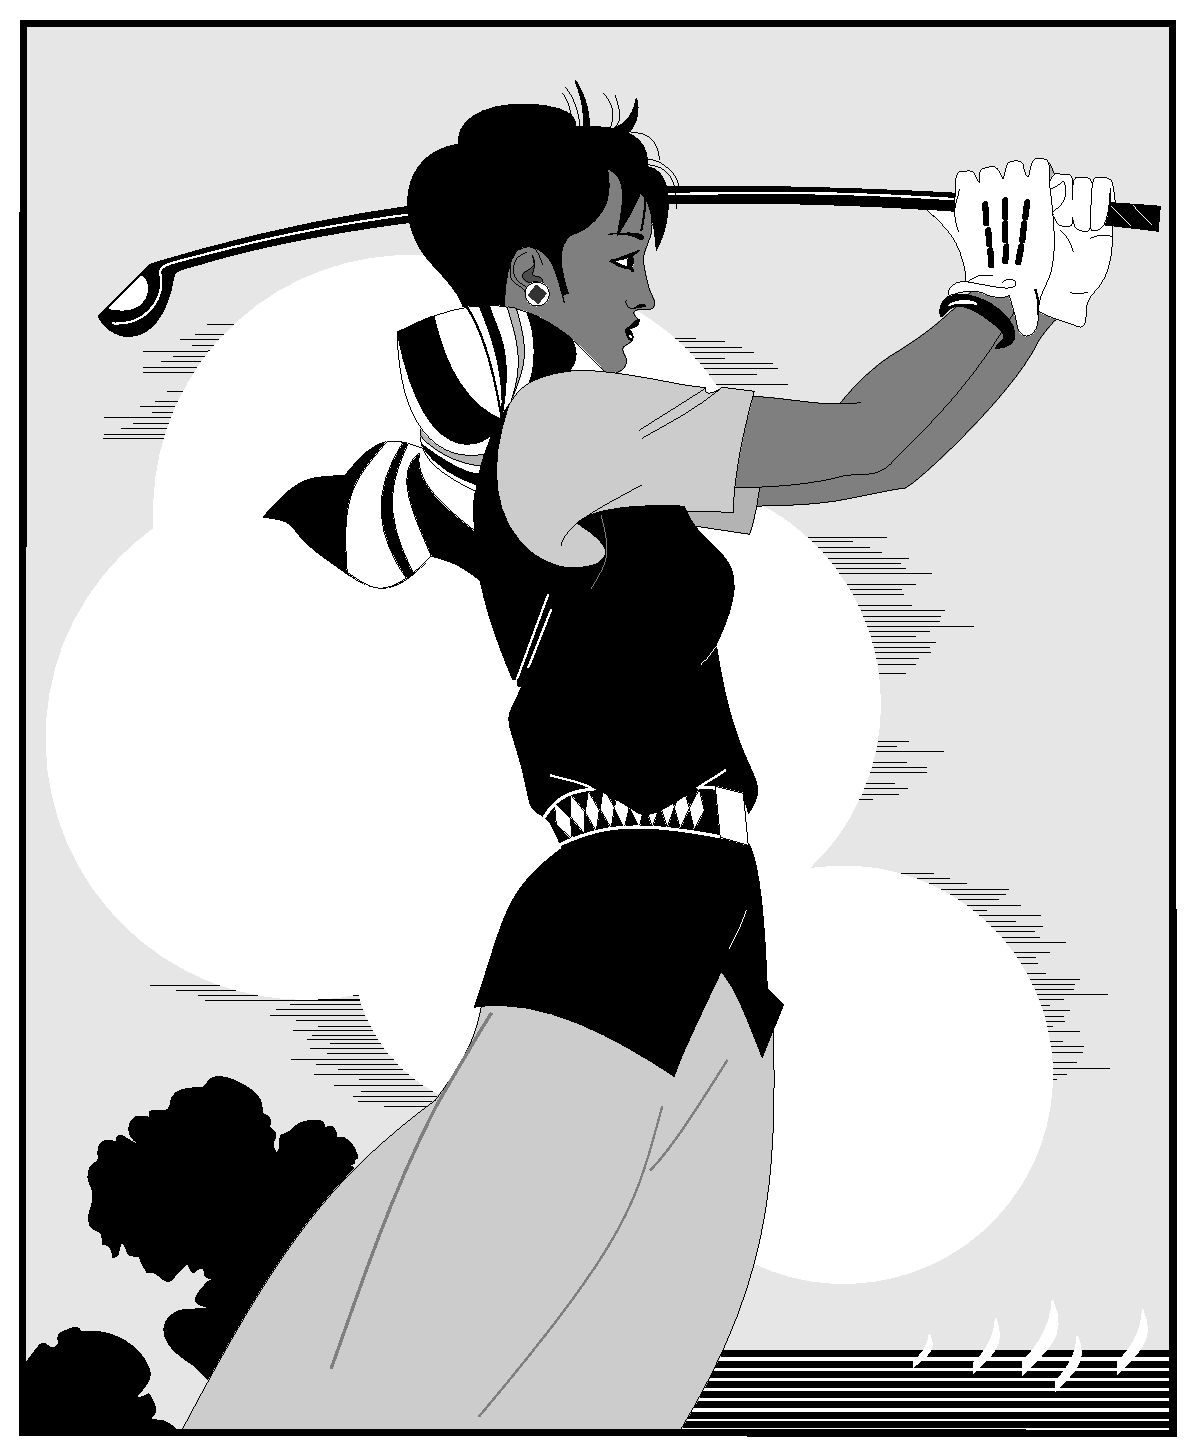
\includegraphics[width = \textwidth]{golfer}\vspace{-5mm}
\FigureBiCaption{打高尔夫球的人test}{Gor Golfer Golfer}
\label{Figure:Tricks:Example1211}
\end{minipage}\hspace{1cm}
\begin{minipage}[t]{0.4\textwidth}
\centering
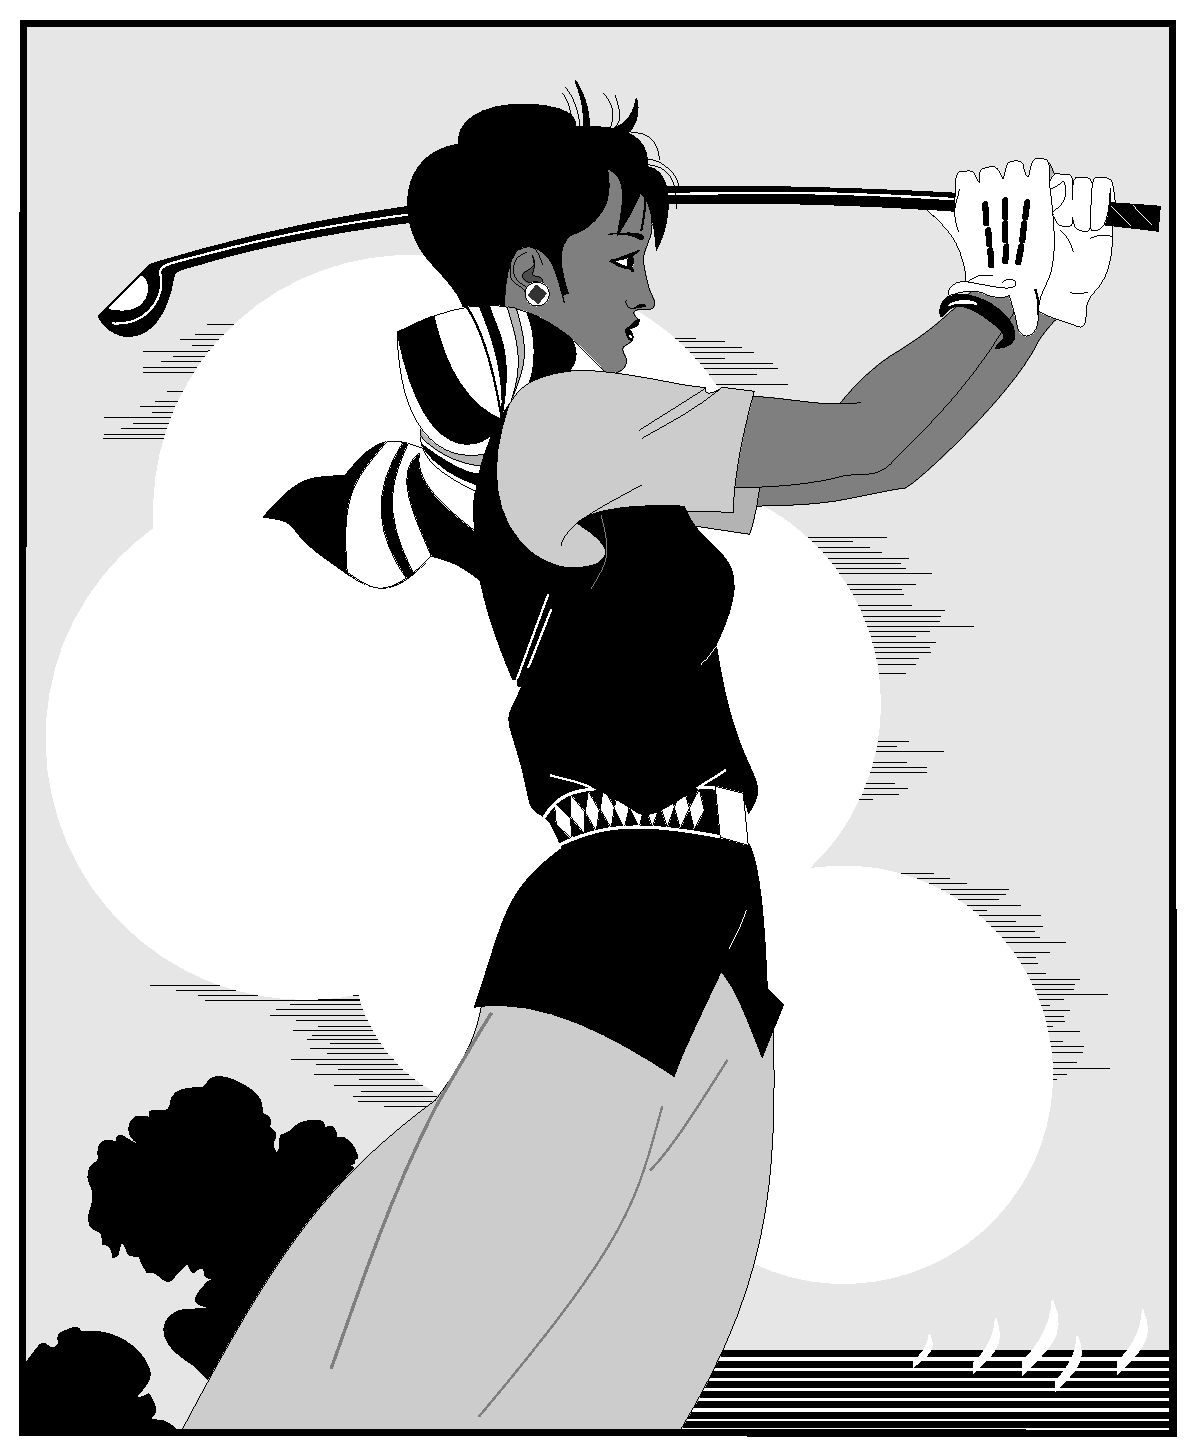
\includegraphics[width = \textwidth]{golfer}\vspace{-5mm}
\FigureBiCaption{打高尔夫球teste2}{Golfer Goolfer Golfer }
\label{Figure:Tricks:Example12222}
\end{minipage}
\end{figure}

% -*-coding: utf-8 -*-

\defaultfont

%%%%%%%%%%%%%%%%%%%%%%%%%%%%%%%%%%%%%%%%%%%%%%%%%%%%%%%%%%%%%%%%%%%%%%%%%%%%%
\BiChapter{版权声明}{Copyright Statement}

本模板遵循~GPL~协议。各贡献者在下面列出:\\
UFO\\
cucme\\
Stanley\\
TeX\\
nebula\\
luckyfox\\
jdg\\
LaTeX\\
还有许多校内校外热心提供帮助解决模板问题的网友朋友们。

% -*-coding: utf-8 -*-

\defaultfont

\BiAppendixChapter{结~~~~论}{Conclusions}
本文提供了一个~\LaTeX~学位论文模板及使用该模板的一些技巧。

如有什么问题,请到哈工大紫丁香~bbs~的~TeX~版发贴。




%%参考文献

% 默认字号
\defaultfont
% 使用 chinesebst2005_UTF8.bst 定义的参考文献格式
\ifx\atempxetex\usewhat
  \bibliographystyle{chinesebst2005_UTF8}
\else
  \bibliographystyle{chinesebst2005_UTF8}
\fi


% 分别把参考文献加入到中英文目录中

\addcontentsline{toc}{chapter}{\hei \ReferenceCName}
\addcontentsline{toe}{chapter}{\bfseries \xiaosi \ReferenceEName}


% 减小参考文献的间距

\addtolength{\bibsep}{-0.8 em} \nocite{*}


% 参考文献

\bibliography{reference/reference}



%英文图形和表格索引里加入空白行,通常放在 % -*-coding: utf-8 -*-

\defaultfont
\appendix

%%%%%%%%%%%%%%%%%%%%%%%%%%%%%%%%%%%%%%%%%%%%%%%%%%%%%%%%%
\BiAppChapter{带章节的附录}{Full Appendix}%
完整的附录内容,包含章节,公式,图表等

%%%%%%%%%%%%%%%%%%%%%%%%%%%%%%%%%%%%%%%%%%%%%%%%%%%%%%%%%
\BiSection{附录节的内容}{Section in Appendix}
这是附录的节的内容

附录中图的示例:
\begin{figure}[h]
\centering
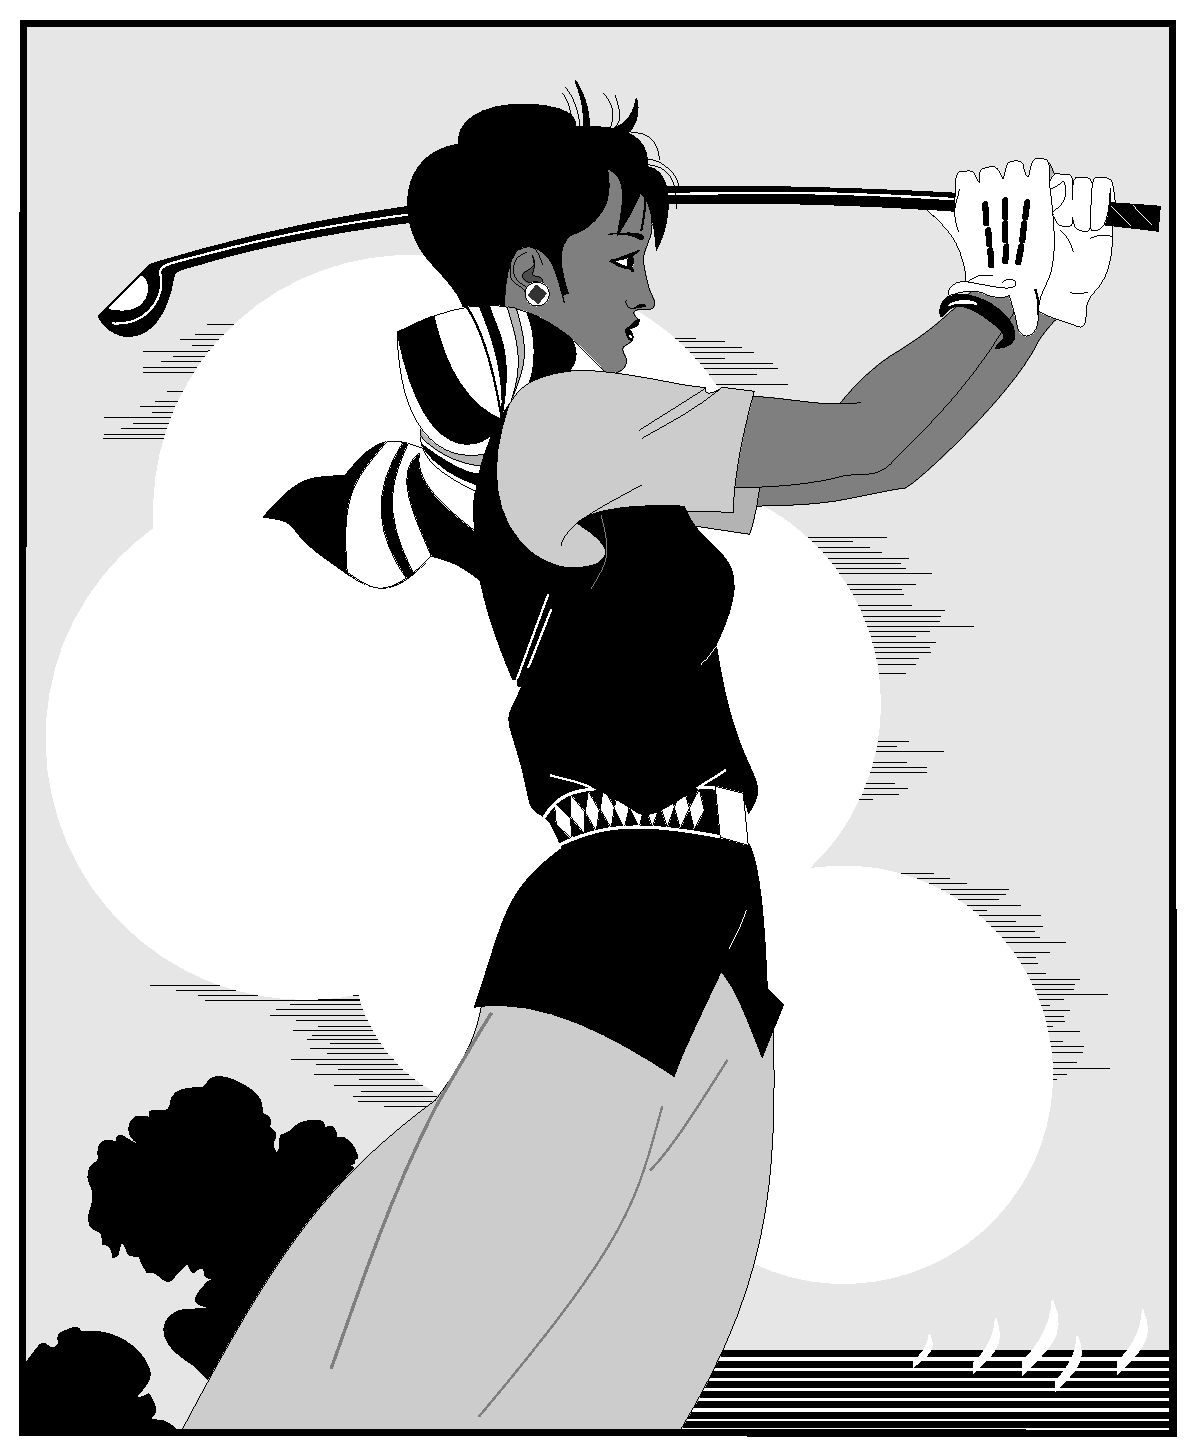
\includegraphics[width = 0.3\textwidth]{golfer}
\FigureBiCaption{打高尔夫球的人}{Golfer}
\label{Figure:Appendix:Example1}
\end{figure}

附录中公式的示例:
\begin{align}
a & = b \times c \\
E & = m c^2
\end{align}

%\BiAppChapter{附录二}{appendix 2}
%\BiAppChapter{附录三}{appendix 3}% 附录A之前。
%区分开正文和附录的图形和表格,一般没有这个必要。
%\addtocontents{fen}{\protect\vskip1\baselineskip}
%\addtocontents{ten}{\protect\vskip1\baselineskip}



% 作品, 承诺, 致谢, 附录, 简历

%% -*-coding: utf-8 -*-

\defaultfont
\BiAppendixChapter{攻读\cxuewei 学位期间发表的学术论文及其它成果} {Papers
Published in the Period of PH. D. Education}

% 书写格式与参考文献相同,这里手写吧 :-)
% 参见...\Accessories\ThesisCriterion\参考文献国标GB7714-2005.pdf内规定
(一)发表的学术论文
\begin{publist}
\item 作者. 题目. 期刊. 年, 卷(期): 页码

\item 作者. 题目. 期刊. 年, 卷(期): 页码

\item 作者. 题目. 期刊. 年, 卷(期): 页码
\end{publist}

(二)申请及已获得的专利(无专利时此项可以不列出)


(三)获得的科技奖励(无获奖时此项不必列出)


% 注:
% 如已发表的学术论文被EI或SCI收录,请标明收录号及SCI论文的影响因子;
% 对已接收但尚未发表出来的学术论文,请注明是否EI或SCI刊源。




    % 所发文章
%% -*-coding: utf-8 -*-

% 先后有三个版本的 授权书格式


\iffalse   %注释掉第一个,采用第二个;
%  +++++++++ 下面是第一种处理方式  ++++++++++++++++++++++++++
    \newpage
%%%%%%%%%%%%%%%%%%哈尔滨工业大学博(硕)士学位论文原创性声明%%%%%%%%%%%%%%%%%%%
    \BiAppendixChapter{哈尔滨工业大学\cxuewei 学位论文原创性声明}{Statement of Copyright}

    本人郑重声明: 此处所提交的 \cxuewei 学位论文《\chinesethesistitle》,
    是本人在导师指导下, 在哈尔滨工业大学攻读\cxuewei 学位期间独立进行研究工作所取得的成果。据本人所知,论文中除已注明部分外不包含他人已发表或撰写过的研究成果。
    对本文的研究工作做出重要贡献的个人和集体, 均已在文中以明确方式注明。 本声明的
    法律结果将完全由本人承担。
    \vspace{0.5cm}
    \begin{flushright}{
    作者签名:~~~~~~~~~~~~~~~~~~~~~~~~~~~~~~~日期:~~~~~~~~~~~年~~~~~月~~~~~日}
    \end{flushright}

    \vspace{0.3cm}

%%%%%%%%%%%%%%%%%%哈尔滨工业大学博(硕)士学位论文使用授权书%%%%%%%%%%%%%%%%%%%
%\phantomsection
\addcontentsline{toc}{chapter}{\hei 哈尔滨工业大学\cxuewei 学位论文使用授权书}
\addcontentsline{toe}{chapter}{\bfseries\xiaosi Letter of Authorization}
    \begin{center}{\xiaoer \hei \bfseries
                    哈尔滨工业大学\cxuewei 学位论文使用授权书}
    \end{center}

    \vspace{0.4cm}

《\chinesethesistitle》 系本人在哈尔滨工业大学攻读\cxuewei 学位期
间在导师指导下完成的\cxuewei 学位论文。本论文的研究成果归哈尔滨工业大学所有,本
论文的研究内容不得以其它单位的名义发表。本人完全了解哈尔滨工业大学关于保存
、使用学位论文的规定,同意学校保留并向有关部门送交论文的复印件和电子版本,
允许论文被查阅和借阅,同意学校将论文加入《中国优秀博硕士学位论文全文数据库》和编入《中国知识资源总库》。本人授权哈尔滨工业大学,可以采用影印、缩印或其他复制
手段保存论文,可以公布论文的全部或部分内容。

\vspace{1.0cm}
\begin{flushright}{
作者签名:~~~~~~~~~~~~~~~~~~~~~~~~~~~~~~~日期:~~~~~~~~~~~年~~~~~月~~~~~日}
\end{flushright}
\vspace{0.2cm}
\begin{flushright}{
导师签名:~~~~~~~~~~~~~~~~~~~~~~~~~~~~~~~日期:~~~~~~~~~~~年~~~~~月~~~~~日}
\end{flushright}

\newpage

\BiAppendixChapter{哈尔滨工业大学\cxuewei 学位涉密论文管理}{Letter of Secret}

%    \begin{center}{\xiaoer \hei \bfseries
%                    哈尔滨工业大学硕博士学位涉密论文管理}
%    \end{center}
%    \vspace{0.4cm}
%\addcontentsline{toc}{chapter}{\hei 哈尔滨工业大学\cxuewei 学位涉密论文管理}
%\addcontentsline{toe}{chapter}{\bfseries\xiaosi Letter of Secret}

根据《哈尔滨工业大学关于国家秘密载体保密管理的规定》,毕业论文答辩必须由导师进行保密初审,外寄论文由科研处复审。涉密毕业论文,由学生按学校规定的统一程序在导师指导下填报密级和保密期限。

 \vspace{0.5cm}
~~~~~~~~~~~~~~~~~~~~~~~~~~~~~~~保密$\square$,在~~~~年解密后适用本授权书。

本学位论文属于

~~~~~~~~~~~~~~~~~~~~~~~~~~~~~~不保密 $\square$ 。

(请在以上相应方框内打“$\surd$”)
\vspace{1.0cm}

\begin{flushright}{
作者签名:~~~~~~~~~~~~~~~~~~~~~~~~~~~~~~~日期:~~~~~~~~~~~年~~~~~月~~~~~日}
\end{flushright} %\vspace{0.2cm}
\begin{flushright}{
导师签名:~~~~~~~~~~~~~~~~~~~~~~~~~~~~~~~日期:~~~~~~~~~~~年~~~~~月~~~~~日}
\end{flushright}

\fi  %注释掉第一个,采用第二个;

%+++++++++++++++++++++++第二种处理方式 by pineapple ++++++++++++++++++++++++++++++++
 \iffalse %% 如果不使用这种方式,去掉 \iffalse \fi 前面的注释
%%%%%%%%%%%%%%%%%%%%%%%%%%%%%%%%%%%%%%%%%%%%%%%%%%%%%%%%%%%%%%%%%%%%%%%%%%%%%%%%
% authorization.tex
%
% Authorization for Use with the Pluto Master Template
%
% Copyright (C) 2006 LIU Yu <pineapple.liu@gmail.com>
%
% This work may be distributed and/or modified under the conditions of the LaTeX
% Project Public License, either version 1.3 of this license or (at your option)
% any later version.
% The latest version of this license is in
%   http://www.latex-project.org/lppl.txt
% and version 1.3 or later is part of all distributions of LaTeX version
% 2005/12/01 or later.
%
% This work has the LPPL maintenance status `unmaintained'.
%
% This work consists of the file(s) authorization.tex
%%%%%%%%%%%%%%%%%%%%%%%%%%%%%%%%%%%%%%%%%%%%%%%%%%%%%%%%%%%%%%%%%%%%%%%%%%%%%%%%

\newpage
\markboth{哈尔滨工业大学\cxuewei 学位论文原创性声明}{哈尔滨工业大学\cxueke\cxuewei 学位论文}

\vspace*{0.1cm}
\newcommand{\subchapterstyle}%
  {\CJKfamily{hei}\rmfamily\bfseries\fontsize{16bp}{16bp}\selectfont}

%\phantomsection
\addcontentsline{toc}{chapter}{\hei 哈尔滨工业大学\cxuewei 学位论文原创性声明}
\addcontentsline{toe}{chapter}{\bfseries\xiaosi Statement of Copyright}
\begin{center}{\subchapterstyle 哈尔滨工业大学\cxuewei 学位论文原创性声明}\end{center}

    本人郑重声明:此处所提交的\cxuewei 学位论文《\chinesethesistitle》 ,是本人在导师指导下,在哈尔滨工业大学攻读\cxuewei 学位期间独立进行研究工作所取得的成果。据本人所知,论文中除已注明部分外不包含他人已发表或撰写过的研究成果。对本文的研究工作做出重要贡献的个人和集体,均已在文中以明确方式注明。本声明的法律结果将完全由本人承担。

\begin{flushright}

作者签字:~~~~~~~~~~~~~~~~~~~~~~~~~~~~~~~~~~~日期:~~~~~~~~~年~~~~~~月~~~~~~日~~~~

\end{flushright}

%\phantomsection
\addcontentsline{toc}{chapter}{\hei 哈尔滨工业大学\cxuewei 学位论文使用授权书}
\addcontentsline{toe}{chapter}{\bfseries\xiaosi Letter of Authorization}
\begin{center}{\subchapterstyle 哈尔滨工业大学\cxuewei 学位论文使用授权书}\end{center}

    《\chinesethesistitle》 系本人在哈尔滨工业大学攻读\cxuewei 学位期间在导师指导下完成的\cxuewei 学位论文。本论文的研究成果归哈尔滨工业大学所有,本论文的研究内容不得以其它单位的名义发表。本人完全了解哈尔滨工业大学关于保存、使用学位论文的规定,同意学校保留并向有关部门送交论文的复印件和电子版本,允许论文被查阅和借阅,同意学校将论文加入《中国优秀博硕士学位论文全文数据库》和编入《中国知识资源总库》。本人授权哈尔滨工业大学,可以采用影印、缩印或其他复制手段保存论文,可以公布论文的全部或部分内容。

\begin{flushright}

作者签名:~~~~~~~~~~~~~~~~~~~~~~~~~~~~~~~~~~~日期:~~~~~~~~~年~~~~~~月~~~~~~日~~~~

导师签名:~~~~~~~~~~~~~~~~~~~~~~~~~~~~~~~~~~~日期:~~~~~~~~~年~~~~~~月~~~~~~日~~~~

\end{flushright}

%\phantomsection
\addcontentsline{toc}{chapter}{\hei 哈尔滨工业大学\cxuewei 学位涉密论文管理} %研究生院说明:暂时不要添加到目录中去,
\addcontentsline{toe}{chapter}{\bfseries\xiaosi Letter of Secret}              %格式也没有完全规定,这里放到下一页上。

\begin{center}{\subchapterstyle 哈尔滨工业大学\cxuewei 学位涉密论文管理}\end{center}

    根据《哈尔滨工业大学关于国家秘密载体保密管理的规定》,毕业论文答辩必须由导师进行保密初审,外寄论文由科研处复审。涉密毕业论文,由学生按学校规定的统一程序在导师指导下填报密级和保密期限。

\begin{flushright}

本学位论文属于~~~~~~~~~~~~~~~~~~~保密$\square$,在~~~~~~~~~~~~年解密后适用本授权书。~~~~~

不保密
$\square$。~~~~~~~~~~~~~~~~~~~~~~~~~~~~~~~~~~~~~~~~~~~~~~~~~~~~~~~~~~~~~~

(请在以上相应方框内打“$\surd$”)~~~~~~~~~~~~~~~~~~~~~~~~~~~~~~~~~~~~~~~~~~~~~~~~~~~~~~~~~~~~~~~~~~~~~~~

\end{flushright}
\begin{flushright}

作者签名:~~~~~~~~~~~~~~~~~~~~~~~~~~~~~~~~~~~日期:~~~~~~~~~年~~~~~~月~~~~~~日~~~~

导师签名:~~~~~~~~~~~~~~~~~~~~~~~~~~~~~~~~~~~日期:~~~~~~~~~年~~~~~~月~~~~~~日~~~~

\end{flushright}
 \fi

%% 第三种处理方式  author: jdg
% \iffalse
\newpage
\markboth{哈尔滨工业大学\cxuewei 学位论文原创性声明}{哈尔滨工业大学\cxueke\cxuewei 学位论文}

\vspace*{0cm}
\newcommand{\subchapterstyle}%
  {\CJKfamily{hei}\rmfamily\bfseries\fontsize{16bp}{16bp}\selectfont}

%\phantomsection
\addcontentsline{toc}{chapter}{\hei 哈尔滨工业大学\cxuewei 学位论文原创性声明}
\addcontentsline{toe}{chapter}{\bfseries\xiaosi Statement of Copyright}
\begin{center}{\subchapterstyle 哈尔滨工业大学\cxuewei 学位论文原创性声明}\end{center}

    本人郑重声明:此处所提交的\cxuewei 学位论文《\chinesethesistitle》 ,是本人在导师指导下,在哈尔滨工业大学攻读\cxuewei 学位期间独立进行研究工作所取得的成果。据本人所知,论文中除已注明部分外不包含他人已发表或撰写过的研究成果。对本文的研究工作做出重要贡献的个人和集体,均已在文中以明确方式注明。本声明的法律结果将完全由本人承担。

\begin{flushright}

作者签名:~~~~~~~~~~~~~~~~~~~~~~~~~~~~~~~~~~~日期:~~~~~~~~~年~~~~~~月~~~~~~日~~~~

\end{flushright}

\vspace{0.4cm}
%\phantomsection
\addcontentsline{toc}{chapter}{\hei 哈尔滨工业大学\cxuewei 学位论文使用授权书}
\addcontentsline{toe}{chapter}{\bfseries\xiaosi Letter of Authorization}
\begin{center}{\subchapterstyle 哈尔滨工业大学\cxuewei 学位论文使用授权书}\end{center}

    《\chinesethesistitle》 系本人在哈尔滨工业大学攻读\cxuewei 学位期间在导师指导下完成的\cxuewei 学位论文。本论文的研究成果归哈尔滨工业大学所有,本论文的研究内容不得以其它单位的名义发表。本人完全了解哈尔滨工业大学关于保存、使用学位论文的规定,同意学校保留并向有关部门送交论文的复印件和电子版本,允许论文被查阅和借阅,同意学校将论文加入《中国优秀博硕士学位论文全文数据库》和编入《中国知识资源总库》。本人授权哈尔滨工业大学,可以采用影印、缩印或其他复制手段保存论文,可以公布论文的全部或部分内容。

\vspace{0.6cm}
本学位论文属于(请在以下相应方框内打“$\surd$”):

保密$\square$,在~~~~~~~~~~~~~年解密后适用本授权书

不保密$\square$

\begin{flushright}{
作者签名:~~~~~~~~~~~~~~~~~~~~~~~~~~~~~~~~~~~日期:~~~~~~~~~年~~~~~~月~~~~~~日~~~~}
\end{flushright} %\vspace{0.2cm}
\begin{flushright}{
导师签名:~~~~~~~~~~~~~~~~~~~~~~~~~~~~~~~~~~~日期:~~~~~~~~~年~~~~~~月~~~~~~日~~~~}
\end{flushright}
%\fi   % 承诺
% -*-coding: utf-8 -*-

\defaultfont

\BiAppendixChapter{致~~~~谢}{Acknowledgements}

该论文模板是UFO@bbs.hit.edu.cn的《哈尔滨工业大学大学博士(硕士)论文模板》的基础上,
并在很多人的帮助下完成的,在此一并向他们表示感谢。

特别感谢Stanley创立了论文模板开源项目Pluto以及他对论文模板的大量修改,
使之更加符合工大论文模板要求。

特别感谢哈工大紫丁香站的~Tex~的版主~Tex、nebula和网友cucme,
他们自始至终都全力支持模板的制作,并为此作了大量的工作。

感谢邓年春~(HIT bbs ID: dengnch),他花了大量的时间来精调模板的
一系列参数,使得该~\LaTeX~模板和对应的~Word~模板的格式几乎完全一致。

感谢水木清华的~\TeX~和~\LaTeX~版的各位网友为我提供的各种帮助,
特别是~snoopyzhao~网友,他多次热心地为该模板解决各种困难,使得模板的制作得以
顺利进行。

最后,衷心感谢哈工大紫丁香~bbs~站~Tex~版所有网友的大力支持!



值此论文完成之际,谨向给予我无私帮助的老师和同学们致以诚挚的谢意!

首先感谢我的导师{\bf 某某某}教授,本论文的研究工作正是在{\bf
某}老师最初的建议下展开的。
他在学术上不断进取、对人生理想执着追求的精神是我学习的榜样。{\bf
某}老师对问题深刻的认识和深入浅出的讲解给我留下深刻印象。


感谢{\bf 某某某}教授和{\bf 某某某}教授对我学习和工作的帮助,
他们勤奋的工作作风、达观的人生态度都深深地感染了我。感谢{\bf
某某某}教授和{\bf 某某某}教授对我学业和生活上的关心。


感谢博士生{\bf 某某某}、{\bf 某某某}、{\bf 某某某}、{\bf 某某某},
给我的无私帮助和积极支持。感谢实验室所有的兄弟姐妹们,
陪伴我度过了这长久的学习、研究阶段,帮助我解决问题,开拓思想。

最后,特别要感谢我的亲人们,他们对我要求甚少,但给予我的都是关怀、支持和理解。
 % 致谢
% -*-coding: utf-8 -*-

\defaultfont
\appendix

%%%%%%%%%%%%%%%%%%%%%%%%%%%%%%%%%%%%%%%%%%%%%%%%%%%%%%%%%
\BiAppChapter{带章节的附录}{Full Appendix}%
完整的附录内容,包含章节,公式,图表等

%%%%%%%%%%%%%%%%%%%%%%%%%%%%%%%%%%%%%%%%%%%%%%%%%%%%%%%%%
\BiSection{附录节的内容}{Section in Appendix}
这是附录的节的内容

附录中图的示例:
\begin{figure}[h]
\centering
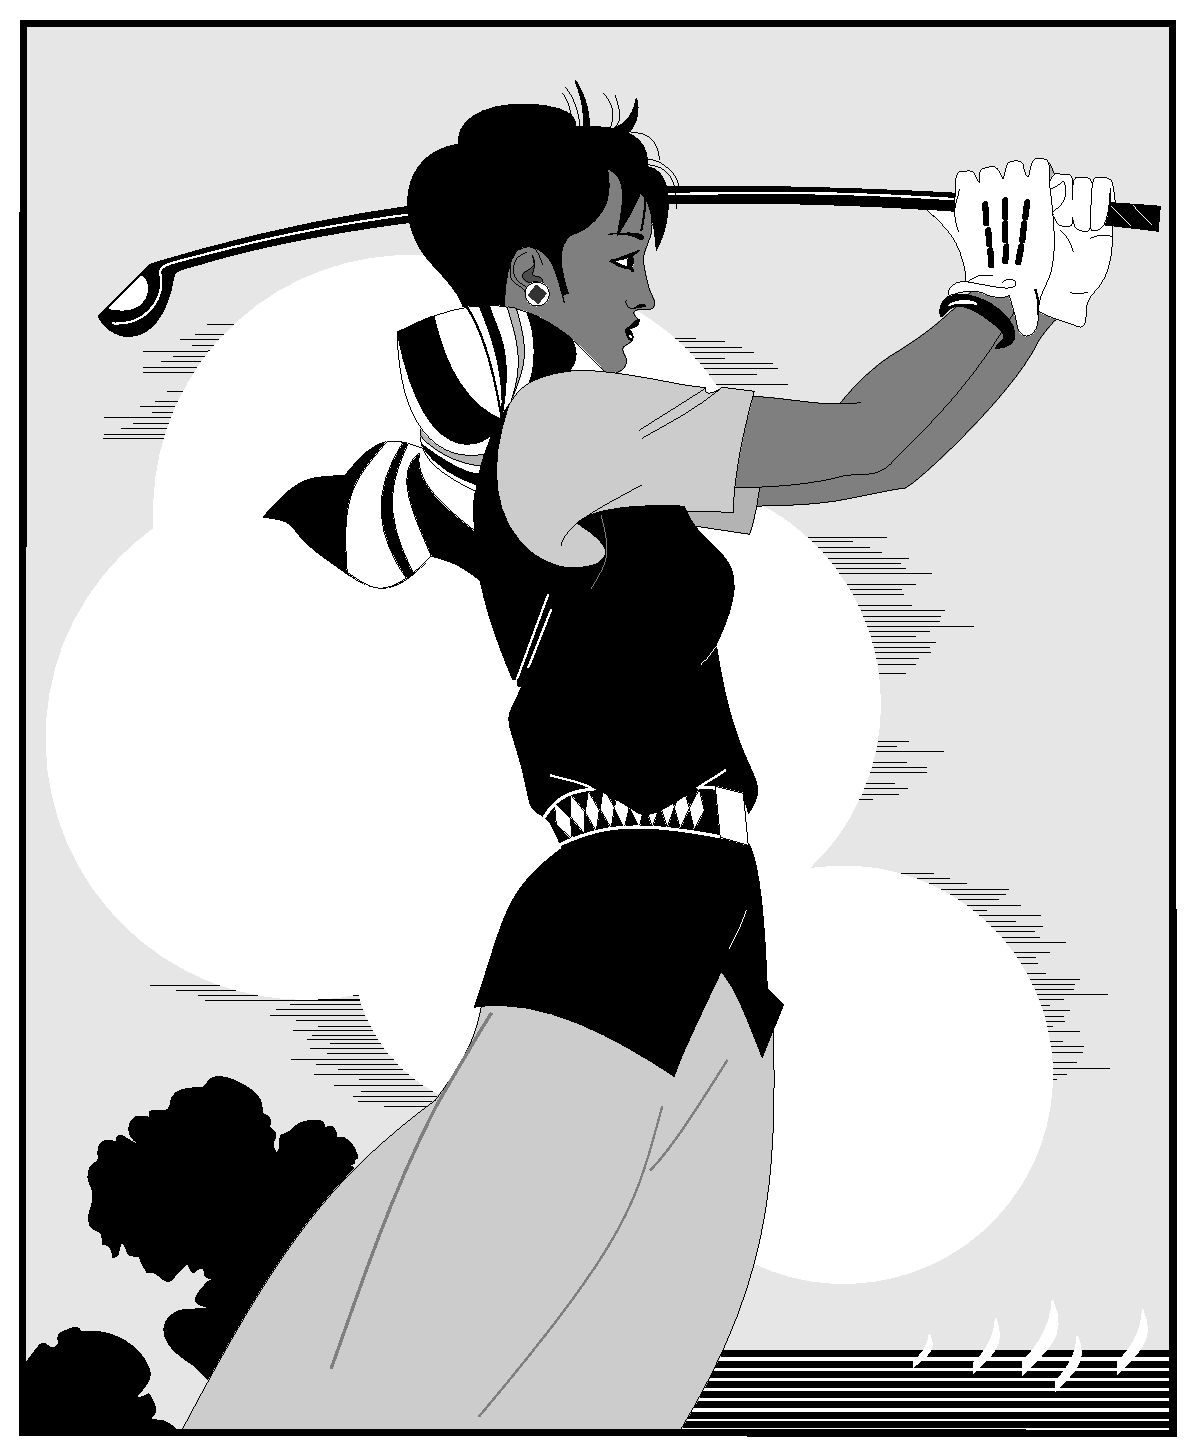
\includegraphics[width = 0.3\textwidth]{golfer}
\FigureBiCaption{打高尔夫球的人}{Golfer}
\label{Figure:Appendix:Example1}
\end{figure}

附录中公式的示例:
\begin{align}
a & = b \times c \\
E & = m c^2
\end{align}

%\BiAppChapter{附录二}{appendix 2}
%\BiAppChapter{附录三}{appendix 3}             % 附录A
%% -*-coding: utf-8 -*-

\defaultfont

\BiAppendixChapter{个人简历}{Resume}

{\hei 学习经历}
\begin{publist}
\item xxxx~年~x~月--至今~~哈尔滨工业大学xxxxxxxxx系~~~攻读工学博士学位
\item xxxx~年~x~月~~~xxxxxxx大学xxxxxxxxxxxxxxxxxx系~~~获工学硕士学位
\item xxxx~年~x~月~~~xxxxxxx大学xxxxxxxxxxxxxxxxxx系~~~获工学学士学位
\end{publist}

{\hei 工作经历}
\begin{publist}
\item xxxx~年~x~月--xxxx~年~x~月  单位  职务
\item xxxx~年~x~月--xxxx~年~x~月  单位  职务
\end{publist}

{\hei 科研工作}
\begin{publist}
\item  xxxx~年~x~月--xxxx~年~x~月 ~~~ xxxx项目~~~~(编号xxx-xxx-xxx) 
\item  xxxx~年~x~月--xxxx~年~x~月 ~~~ xxxx项目~~~~(编号xxx-xxx-xxx)
\item  xxxx~年~x~月--xxxx~年~x~月 ~~~ xxxx项目~~~~(编号xxx-xxx-xxx)
\item  xxxx~年~x~月--xxxx~年~x~月 ~~~ xxxx项目~~~~(编号xxx-xxx-xxx)
\end{publist}

{\hei 学术论文}
\begin{publist}
\item 在~xxxxxxx~等刊物发表论文多篇
\item 在~xxxxxxxxxxxxxxxx~等多个国际会议上发表论文多篇
\end{publist}

{\hei 专利情况}
\begin{publist}
\item 作者. 产品名称. 专利名称(专利号:XXXXXXX), 年。
\item 作者. 产品名称. 专利名称(专利号:XXXXXXX), 年。
\end{publist}
          % 个人简历



\clearpage



% 如果使用 xelatex 方式编译, 结束 CJK 环境

\ifx\atempxetex\usewhat
\else
\end{CJK*}
\fi



% 文档结束

\end{document}



%%% Local Variables: 
%%% mode: latex
%%% TeX-master: t
%%% End: 
